\documentclass[twocolumn,superscriptaddress,prd]{revtex4-1} 

\pdfoutput=1 

%\usepackage{hyperref}
\usepackage{verbatim}
%\usepackage[font=normalsize]{caption}
\usepackage{mathtools}
\usepackage{relsize}
\usepackage{natbib}

\usepackage{amsmath}
\usepackage{graphicx}
\usepackage[capposition=bottom]{floatrow}
\usepackage{amssymb}
\usepackage{graphicx}
%\usepackage{caption}
\usepackage{rotating}
\usepackage{afterpage}
\usepackage{float}
\usepackage{geometry}
\usepackage{titlesec}
\usepackage{epstopdf}

\usepackage{latexsym}
\usepackage{graphicx}
\usepackage{color}
\usepackage{array}
\usepackage{multirow}
\usepackage{wasysym}
\usepackage{verbatim}
\usepackage{subfig}


%switch from two to one column



\addtolength{\oddsidemargin}{-.500in}
\addtolength{\evensidemargin}{-.375in}
\addtolength{\textwidth}{1.00in}
%\addtolength{\voffset}{-70pt}
%\addtolength{\textheight} {120pt}
\newcommand{\isot}[2]{$^{#2}$#1 }
\newcommand{\xeiso}{\isot{Xe}{136}}
\newcommand{\thsrc}{\isot{Th}{228}}
\newcommand{\cosrc}{\isot{Co}{60}}
\newcommand{\krsrc}{\isot{Kr}{83m}}
\newcommand{\cssrc}{\isot{Cs}{137}}
\newcommand{\kevee}{keV$_{ee}$ }
\newcommand{\nonubb}  {$0\nu \beta \beta$}
\newcommand{\gone}{$0.116 \pm 0.003$}
\newcommand{\gtwo}{$11.41 \pm 0.52$}
\newcommand{\fixit}[1]{{\color{red}#1}} 

\renewcommand\thesection{\Roman{section}.}
\renewcommand\thesubsection{\arabic{subsection}.}
\renewcommand\thesubsubsection{\alph{subsubsection}.}
\titleformat{\section}[block]{\bfseries\filcenter}{\thesection}{1em}{}
\titleformat{\subsection}[block]{\bfseries\filcenter}{\thesubsection}{1em}{}
\titleformat{\subsubsection}{\bfseries\filcenter}{\thesubsubsection}{1em}{}

\usepackage{titlesec}

%\titleformat{\section}{\bfseries\filcenter}{\thesubsection}{1em}{}
%\titleformat{\subsection}{\bfseries\filcenter}{\thesubsection}{1em}{}
%\titleformat*{\paragraph}{\large\bfseries}
%\titleformat*{\subparagraph}{\large\bfseries}

\begin{document}

\title{Tritium calibration of the LUX dark matter experiment}

\author{D.S.~Akerib} %% Joined 4/2008
\affiliation{Case Western Reserve University, Dept. of Physics, 10900 Euclid Ave, Cleveland OH 44106, USA}
\affiliation{SLAC National Accelerator Laboratory, 2575 Sand Hill Road, Menlo Park CA 94205-7015, USA}
\affiliation{Kavli Institute for Particle Astrophysics and Cosmology, Stanford University, 452 Lomita Mall, Stanford, CA 94309, USA}

\author{H.M.~Ara\'{u}jo} %% Joined 4/2012, Author on 4/2013
\affiliation{Imperial College London, High Energy Physics, Blackett Laboratory, London SW7 2BZ, UK}

\author{X.~Bai} %% Joined 7/2009
\affiliation{South Dakota School of Mines and Technology, 501 East St Joseph St., Rapid City SD 57701, USA}

\author{A.J.~Bailey} %% Joined 1/2013, Author on 1/2014
\affiliation{Imperial College London, High Energy Physics, Blackett Laboratory, London SW7 2BZ, UK}

\author{J.~Balajthy} %% Joined 7/2012, Author on 7/2013
\affiliation{University of Maryland, Dept. of Physics, College Park MD 20742, USA}

%\author{S.~Bedikian} %% Left 2/2010, Author until 2/2012
%\affiliation{Yale University, Dept. of Physics, 217 Prospect St., New Haven CT 06511, USA}

\author{P.~Beltrame} %% Joined 10/2013, Author on 10/2014.
\affiliation{SUPA, School of Physics and Astronomy, University of Edinburgh, Edinburgh, EH9 3FD, UK}

\author{E.P.~Bernard} %% Joined 1/2010, Author on 1/2011
\affiliation{Yale University, Dept. of Physics, 217 Prospect St., New Haven CT 06511, USA}

\author{A.~Bernstein} %% From the start
\affiliation{Lawrence Livermore National Laboratory, 7000 East Ave., Livermore CA 94551, USA}

\author{T.P.~Biesiadzinski} %% Joined 10/2013, Author on 10/2014
\affiliation{Case Western Reserve University, Dept. of Physics, 10900 Euclid Ave, Cleveland OH 44106, USA}
\affiliation{SLAC National Accelerator Laboratory, 2575 Sand Hill Road, Menlo Park CA 94205-7015, USA}
\affiliation{Kavli Institute for Particle Astrophysics and Cosmology, Stanford University, 452 Lomita Mall, Stanford, CA 94309, USA}

%\author{A.~Bolozdynya} %% From the start, Left Case 7/09, Author until 7/11
%\affiliation{Case Western Reserve University, Dept. of Physics, 10900 Euclid Ave, Cleveland OH 44106, USA}

\author{E.M.~Boulton} %% Joined 3/2013, Author on 3/2014
\affiliation{Yale University, Dept. of Physics, 217 Prospect St., New Haven CT 06511, USA}

\author{A.~Bradley} %% From start, Left 12/2013, Author until 12/2015
\affiliation{Case Western Reserve University, Dept. of Physics, 10900 Euclid Ave, Cleveland OH 44106, USA}

\author{R.~Bramantei} %% Joined 3/2014, Author on 3/2015
\affiliation{Case Western Reserve University, Dept. of Physics, 10900 Euclid Ave, Cleveland OH 44106, USA}
\affiliation{SLAC National Accelerator Laboratory, 2575 Sand Hill Road, Menlo Park CA 94205-7015, USA}
\affiliation{Kavli Institute for Particle Astrophysics and Cosmology, Stanford University, 452 Lomita Mall, Stanford, CA 94309, USA}

%\author{D.~Byram} %% Joined 10/2010, Left 3/2013, Author until 3/2015
%\affiliation{University of South Dakota, Dept. of Physics, 414E Clark St., Vermillion SD 57069, USA}

\author{S.B.~Cahn} %% Joined 2/2009, Left 12/2012, Worked on Kr source in 2015, Author until 12/2017
\affiliation{Yale University, Dept. of Physics, 217 Prospect St., New Haven CT 06511, USA}

\author{M.C.~Carmona-Benitez} %% Joined 10/2009, Moved from Case to UCSB 7/31/2013
\affiliation{University of California Santa Barbara, Dept. of Physics, Santa Barbara, CA, USA}

%\author{D. Carr}{ %% From start, Left on ??
%\affiliation{Lawrence Livermore National Laboratory, 7000 East Ave., Livermore CA 94551, USA}}

\author{C.~Chan} %% Joined 8/2012, Author on 8/2013
\affiliation{Brown University, Dept. of Physics, 182 Hope St., Providence RI 02912, USA}

\author{J.J.~Chapman} %% Joined 6/2007, Author on 6/2008, Left on 1/2014, Author until 1/2016
\affiliation{Brown University, Dept. of Physics, 182 Hope St., Providence RI 02912, USA}

\author{A.A.~Chiller} %% Joined 11/2011, Author on 11/2012
\affiliation{University of South Dakota, Dept. of Physics, 414E Clark St., Vermillion SD 57069, USA}

\author{C.~Chiller} %% Joined 11/2011, Author on 11/2012
\affiliation{University of South Dakota, Dept. of Physics, 414E Clark St., Vermillion SD 57069, USA}

%\author{K.~Clark} %% Joined 6/2008, Left 6/2010, Author until 6/2012
%\affiliation{Case Western Reserve University, Dept. of Physics, 10900 Euclid Ave, Cleveland OH 44106, USA}

%\author{T.~Classen}{ %% Joined 10/2007, Left 11/2009, Author until 11/2011
%  address={University of California Davis, Dept. of Physics, One Shields Ave., Davis CA 95616, USA}}

%\author{T.~Coffey} %% Joined 8/2010, Left 8/2012, Author until 8/2014
%\affiliation{Case Western Reserve University, Dept. of Physics, 10900 Euclid Ave, Cleveland OH 44106, USA}

\author{A.~Currie} %% Joined 4/2012, Author on 4/2013
\affiliation{Imperial College London, High Energy Physics, Blackett Laboratory, London SW7 2BZ, UK}

%\author{A.~Curioni} %% Left 6/2009, Author until 6/2011
%\affiliation{Yale University, Dept. of Physics, 217 Prospect St., New Haven CT 06511, USA}

\author{J.E.~Cutter}  %% Joined 8/2013, Author on 8/2014
\affiliation{University of California Davis, Dept. of Physics, One Shields Ave., Davis CA 95616, USA}

%\author{E.~Dahl}{ %% From start; Left ???
%\affiliation{Case Western Reserve University, Dept. of Physics, 10900 Euclid Ave, Cleveland OH 44106, USA}}

\author{T.J.R.~Davison} %% Joined 2/2014, Author on 2/2015.
\affiliation{SUPA, School of Physics and Astronomy, University of Edinburgh, Edinburgh, EH9 3FD, UK}

%\author{S.~Dazeley} %% From start, Left ?
%\affiliation{Lawrence Livermore National Laboratory, 7000 East Ave., Livermore CA 94551, USA}

\author{L.~de\,Viveiros} %% From the start (at Brown), moved to Coimbra, Left 11/2013, Author until 11/2015. 
\affiliation{LIP-Coimbra, Department of Physics, University of Coimbra, Rua Larga, 3004-516 Coimbra, Portugal}

\author{A.~Dobi} %% Joined 7/2011, Author on 7/2012
\affiliation{Lawrence Berkeley National Laboratory, 1 Cyclotron Rd., Berkeley, CA 94720, USA}

\author{J.E.Y.~Dobson} %% Joined 09/2012, Author on 09/2013, Left 7/2015, Author until 7/2017
\affiliation{Department of Physics and Astronomy, University College London, Gower Street, London WC1E 6BT, UK}

%\author{E.~Dragowsky} %% Joined 01/09, Left 10/11, Author until 10/13
%\affiliation{Case Western Reserve University, Dept. of Physics, 10900 Euclid Ave, Cleveland OH 44106, USA}

\author{E.~Druszkiewicz} %% From the start
\affiliation{University of Rochester, Dept. of Physics and Astronomy, Rochester NY 14627, USA}

\author{B.N.~Edwards} %% Joined 3/2011, Author on 3/2012.
\affiliation{Yale University, Dept. of Physics, 217 Prospect St., New Haven CT 06511, USA}

\author{C.H.~Faham} %% Joined June 2007, Moved from Brown to Berkeley 9/1/2013, Left 6/2015, Author until 6/2017
\affiliation{Lawrence Berkeley National Laboratory, 1 Cyclotron Rd., Berkeley, CA 94720, USA}

\author{S.~Fiorucci} %% From start
\affiliation{Brown University, Dept. of Physics, 182 Hope St., Providence RI 02912, USA}

%\author{C.~Flores} %% Joined 10/2012, Left 10/2012
%\affiliation{University of California Davis, Dept. of Physics, One Shields Ave., Davis CA 95616, USA}

\author{R.J.~Gaitskell} %% From start
\affiliation{Brown University, Dept. of Physics, 182 Hope St., Providence RI 02912, USA}

\author{V.M.~Gehman} %% Joined 5/2012, Author on 5/2013, Left 6/2015, Author until 6/2017
\affiliation{Lawrence Berkeley National Laboratory, 1 Cyclotron Rd., Berkeley, CA 94720, USA}

\author{C.~Ghag} %% Joined 6/2012, Author on 6/2013
\affiliation{Department of Physics and Astronomy, University College London, Gower Street, London WC1E 6BT, UK}

\author{K.R.~Gibson} %% Joined 10/2009, Left 9/2014, Author until 9/2016
\affiliation{Case Western Reserve University, Dept. of Physics, 10900 Euclid Ave, Cleveland OH 44106, USA}

\author{M.G.D.~Gilchriese} %% Joined 10/2010, Author on 10/2011
\affiliation{Lawrence Berkeley National Laboratory, 1 Cyclotron Rd., Berkeley, CA 94720, USA}

\author{C.R.~Hall} %% Joined 3/2008, Author on 3/2009
\affiliation{University of Maryland, Dept. of Physics, College Park MD 20742, USA}

\author{M.~Hanhardt} %% Joined 7/2009, Left 8/2011, Rejoined 7/2013, Author on 7/2014
\affiliation{South Dakota School of Mines and Technology, 501 East St Joseph St., Rapid City SD 57701, USA}
\affiliation{South Dakota Science and Technology Authority, Sanford Underground Research Facility, Lead, SD 57754, USA}

\author{S.J.~Haselschwardt}  %% Joined 6/2013, Author on 6/2014
\affiliation{University of California Santa Barbara, Dept. of Physics, Santa Barbara, CA, USA}

\author{S.A.~Hertel} %% Joined 9/2012, Author on 9/2013
\affiliation{University of California Berkeley, Department of Physics, Berkeley, CA 94720, USA}
\affiliation{Yale University, Dept. of Physics, 217 Prospect St., New Haven CT 06511, USA}

\author{D.P.~Hogan} %% Joined 2/2014, Author on 2/2015
\affiliation{University of California Berkeley, Department of Physics, Berkeley, CA 94720, USA}

%\author{B.~Holbrook}{ %% Engineer, Joined 12/2007
%  address={University of California Davis, Dept. of Physics, One Shields Ave., Davis CA 95616, USA}}

\author{M.~Horn} %% Joined 4/2012, Author on 4/2013.
\affiliation{University of California Berkeley, Department of Physics, Berkeley, CA 94720, USA}
\affiliation{Yale University, Dept. of Physics, 217 Prospect St., New Haven CT 06511, USA}

\author{D.Q.~Huang} %% Joined 7/2012, Author on 7/2013
\affiliation{Brown University, Dept. of Physics, 182 Hope St., Providence RI 02912, USA}

\author{C.M.~Ignarra} %% Joined 10/2014, Author on 10/2015
\affiliation{SLAC National Accelerator Laboratory, 2575 Sand Hill Road, Menlo Park CA 94205-7015, USA}
\affiliation{Kavli Institute for Particle Astrophysics and Cosmology, Stanford University, 452 Lomita Mall, Stanford, CA 94309, USA}

\author{M.~Ihm} %% Joined 10/2009, Author on 10/2010
\affiliation{University of California Berkeley, Department of Physics, Berkeley, CA 94720, USA}

%\author{T. Ivancic}{ %% Joined 1/2012, Left 6/2012, Never an author.
%  address={Case Western Reserve University, Dept. of Physics, 10900 Euclid Ave, Cleveland OH 44106, USA}}

\author{R.G.~Jacobsen} %% Joined 12/2009, Author on 12/2010
\affiliation{University of California Berkeley, Department of Physics, Berkeley, CA 94720, USA}

\author{W.~Ji} %% Joined 3/2014, Author on 3/2015
\affiliation{Case Western Reserve University, Dept. of Physics, 10900 Euclid Ave, Cleveland OH 44106, USA}
\affiliation{SLAC National Accelerator Laboratory, 2575 Sand Hill Road, Menlo Park CA 94205-7015, USA}
\affiliation{Kavli Institute for Particle Astrophysics and Cosmology, Stanford University, 452 Lomita Mall, Stanford, CA 94309, USA}

%\author{K.~Kamdin %% Joined 3/2015, Author on 3/2016
%\affiliation{University of California Berkeley, Department of Physics, Berkeley, CA 94720, USA}

%\author{L.~Kastens} %% Joined 6/2007, Left 7/2011, Author until 7/2013
%\affiliation{Yale University, Dept. of Physics, 217 Prospect St., New Haven CT 06511, USA}

\author{K.~Kazkaz} %% From start
\affiliation{Lawrence Livermore National Laboratory, 7000 East Ave., Livermore CA 94551, USA}

\author{D.~Khaitan} %% Joined 6/2014, Author on 6/2015
\affiliation{University of Rochester, Dept. of Physics and Astronomy, Rochester NY 14627, USA}

\author{R.~Knoche} %% Joined 7/2011, Author on 7/2012
\affiliation{University of Maryland, Dept. of Physics, College Park MD 20742, USA}

%\author{S.~Kyre} %% Engineer, Joined 6/2010
%\affiliation{University of California Santa Barbara, Dept. of Physics, Santa Barbara, CA, USA}

%\author{R.~Lander} %% Joined 3/2008, Decided not to be a LUX author.
%\affiliation{University of California Davis, Dept. of Physics, One Shields Ave., Davis CA 95616, USA}

\author{N.A.~Larsen} %% Joined 6/2010, Author on 6/2011
\affiliation{Yale University, Dept. of Physics, 217 Prospect St., New Haven CT 06511, USA}

\author{C.~Lee} %% Joined 8/2009
\affiliation{Case Western Reserve University, Dept. of Physics, 10900 Euclid Ave, Cleveland OH 44106, USA}
\affiliation{SLAC National Accelerator Laboratory, 2575 Sand Hill Road, Menlo Park CA 94205-7015, USA}
\affiliation{Kavli Institute for Particle Astrophysics and Cosmology, Stanford University, 452 Lomita Mall, Stanford, CA 94309, USA}

\author{B.G.~Lenardo} %% Joined 7/2013, Author on 7/2014
\affiliation{University of California Davis, Dept. of Physics, One Shields Ave., Davis CA 95616, USA}
\affiliation{Lawrence Livermore National Laboratory, 7000 East Ave., Livermore CA 94551, USA}

%\author{D.S.~Leonard} %% Joined 11/2008, Left 2/2010, Author until 2/2012.
%\affiliation{University of Maryland, Dept. of Physics, College Park MD 20742, USA}

\author{K.T.~Lesko} %% Joined 3/2007, Left ?, Rejoined 4/2013, Author on 4/2014
\affiliation{Lawrence Berkeley National Laboratory, 1 Cyclotron Rd., Berkeley CA 94720, USA}

\author{A.~Lindote} %% Joined 12/2010, Author on 12/2011.
\affiliation{LIP-Coimbra, Department of Physics, University of Coimbra, Rua Larga, 3004-516 Coimbra, Portugal}

\author{M.I.~Lopes} %% Joined 12/2010, Author on 12/2011.
\affiliation{LIP-Coimbra, Department of Physics, University of Coimbra, Rua Larga, 3004-516 Coimbra, Portugal}

%\author{R. Lorek}{ %% Joined 6/2012, Focussed on R&D for LZ, Will not be an author.
%  address={Case Western Reserve University, Dept. of Physics, 10900 Euclid Ave, Cleveland OH 44106, USA}}

%\author{A.~Lyashenko} %% Joined 7/2009, Left 8/2011, Author until 8/2013
%\affiliation{Yale University, Dept. of Physics, 217 Prospect St., New Haven CT 06511, USA}

\author{D.C.~Malling} %% Joined 8/2007, Author on 8/2008, Left on 12/2013, Author until 12/2015 
\affiliation{Brown University, Dept. of Physics, 182 Hope St., Providence RI 02912, USA}

\author{A.G.~Manalaysay}{ %% Joined 10/2013, Author on 10/2014
\affiliation{University of California Davis, Dept. of Physics, One Shields Ave., Davis CA 95616, USA}}

\author{R.L.~Mannino} %% Joined 6/2009, Author on 6/2010
\affiliation{Texas A \& M University, Dept. of Physics, College Station TX 77843, USA}

\author{M.F.~Marzioni} %% Joined 9/2014, Author on 9/2015
\affiliation{SUPA, School of Physics and Astronomy, University of Edinburgh, Edinburgh, EH9 3FD, UK}

\author{D.N.~McKinsey} %% Joined 6/2007, Author on 6/2008
\affiliation{University of California Berkeley, Department of Physics, Berkeley, CA 94720, USA}
\affiliation{Yale University, Dept. of Physics, 217 Prospect St., New Haven CT 06511, USA}

\author{D.-M.~Mei} %% Joined 7/2008
\affiliation{University of South Dakota, Dept. of Physics, 414E Clark St., Vermillion SD 57069, USA}

\author{J.~Mock} %% Joined 8/2007
\affiliation{University at Albany, State University of New York, Dept. of Physics, 1400 Washington Ave., Albany, NY 12222, USA}

\author{M.~Moongweluwan} %% Joined 6/2011, Author on 6/2012.
\affiliation{University of Rochester, Dept. of Physics and Astronomy, Rochester NY 14627, USA}

\author{J.A.~Morad} %% Joined 7/2012, Author on 7/2013
\affiliation{University of California Davis, Dept. of Physics, One Shields Ave., Davis CA 95616, USA}

%\author{M.~Morii} %% Joined June 09, Left May 2011, Author until May 2013
%\affiliation{Harvard University, Dept. of Physics, 17 Oxford St., Cambridge MA 02138, USA}

\author{A.St.J.~Murphy} %% Joined 06/2012, Author on 06/2013.
\affiliation{SUPA, School of Physics and Astronomy, University of Edinburgh, Edinburgh, EH9 3FD, UK}

\author{C.~Nehrkorn} %% Joined 5/2012, Author on 5/2013
\affiliation{University of California Santa Barbara, Dept. of Physics, Santa Barbara, CA, USA}

\author{H.N.~Nelson} %% Joined 11/2008
\affiliation{University of California Santa Barbara, Dept. of Physics, Santa Barbara, CA, USA}

\author{F.~Neves} %% Joined 12/2010, Author on 12/2011.
\affiliation{LIP-Coimbra, Department of Physics, University of Coimbra, Rua Larga, 3004-516 Coimbra, Portugal}

%\author{J.A.~Nikkel} %% Joined 4/2008, Left 12/2011, Author until 12/2013
%\affiliation{Yale University, Dept. of Physics, 217 Prospect St., New Haven CT 06511, USA}

\author{K.~O'Sullivan} %% Joined 9/2012, Author on 9/2013
\affiliation{University of California Berkeley, Department of Physics, Berkeley, CA 94720, USA}
\affiliation{Lawrence Berkeley National Laboratory, 1 Cyclotron Rd., Berkeley CA 94720, USA}
\affiliation{Yale University, Dept. of Physics, 217 Prospect St., New Haven CT 06511, USA}

\author{K.C.~Oliver-Mallory} %% Joined 5/2014, Author on 5/2015
\affiliation{University of California Berkeley, Department of Physics, Berkeley, CA 94720, USA}

\author{R.A.~Ott} %% Joined 3/2012, Author on 3/2013, Left on 3/2014, Author until 3/2016
\affiliation{University of California Davis, Dept. of Physics, One Shields Ave., Davis CA 95616, USA}

\author{K.J.~Palladino} %% Joined 10/2013, Author on 10/2014
\affiliation{SLAC National Accelerator Laboratory, 2575 Sand Hill Road, Menlo Park CA 94205-7015, USA}
\affiliation{Kavli Institute for Particle Astrophysics and Cosmology, Stanford University, 452 Lomita Mall, Stanford, CA 94309, USA}

\author{M.~Pangilinan} %% Joined 2/2010, Left  4/2014, Author until 4/2016
\affiliation{Brown University, Dept. of Physics, 182 Hope St., Providence RI 02912, USA}

%\author{P.D.~Parker} %% Joined 9/2010, Active on 12/2011, Left on 6/2013, Author until 6/2015
%\affiliation{Yale University, Dept. of Physics, 217 Prospect St., New Haven CT 06511, USA}

\author{E.K.~Pease} %% Joined 12/2011, Author on 12/2012.
\affiliation{Yale University, Dept. of Physics, 217 Prospect St., New Haven CT 06511, USA}

%\author{K.~Pech} %% Joined 6/2011, Author on 6/2012, Left 9/2013, Author until 9/2015
%\affiliation{Case Western Reserve University, Dept. of Physics, 10900 Euclid Ave, Cleveland OH 44106, USA}

\author{P.~Phelps} %% Joined 6/2008, Left 7/2014, Author until 7/2016
\affiliation{Case Western Reserve University, Dept. of Physics, 10900 Euclid Ave, Cleveland OH 44106, USA}

%\author{J.~Pinto~da~Cunha}{ %% Joined 12/2010, will not be an author until further notice.
%\affiliation{LIP-Coimbra, Department of Physics, University of Coimbra, Rua Larga, 3004-516 Coimbra, Portugal}}

\author{L.~Reichhart} %% Joined 6/2012, Author on 6/2013, Left on 5/2015, Author until 5/2017
\affiliation{Department of Physics and Astronomy, University College London, Gower Street, London WC1E 6BT, UK}

\author{C.~Rhyne} %% Joined 6/2014, Author on 6/2015
\affiliation{Brown University, Dept. of Physics, 182 Hope St., Providence RI 02912, USA}

\author{S.~Shaw} %% Joined 2/2014, Author on 2/2015
\affiliation{Department of Physics and Astronomy, University College London, Gower Street, London WC1E 6BT, UK}

\author{T.A.~Shutt} %% From start
\affiliation{Case Western Reserve University, Dept. of Physics, 10900 Euclid Ave, Cleveland OH 44106, USA}
\affiliation{SLAC National Accelerator Laboratory, 2575 Sand Hill Road, Menlo Park CA 94205-7015, USA}
\affiliation{Kavli Institute for Particle Astrophysics and Cosmology, Stanford University, 452 Lomita Mall, Stanford, CA 94309, USA}

\author{C.~Silva} %% Joined 12/2010, Author on 12/2011.
\affiliation{LIP-Coimbra, Department of Physics, University of Coimbra, Rua Larga, 3004-516 Coimbra, Portugal}

%\author{W.~Skulski} %% From start, Author on trigger-related publications.
%\affiliation{University of Rochester, Dept. of Physics and Astronomy, Rochester NY 14627, USA}

\author{V.N.~Solovov} %% Joined 12/2010, Author on 12/2011.
\affiliation{LIP-Coimbra, Department of Physics, University of Coimbra, Rua Larga, 3004-516 Coimbra, Portugal}

\author{P.~Sorensen} %% From start
\affiliation{Lawrence Berkeley National Laboratory, 1 Cyclotron Rd., Berkeley, CA 94720, USA}

%\author{J. Spaans} %% Joined 2/2009, Left 5/2010, Author until 5/2012
%\affiliation{University of South Dakota, Dept. of Physics, 414E Clark St., Vermillion SD 57069, USA}}

\author{S.~Stephenson}  %% Joined 8/2014, Author on 8/2015
\affiliation{University of California Davis, Dept. of Physics, One Shields Ave., Davis CA 95616, USA}

%\author{T. Stiegler} %% Joined 10/2007, Left on 12/2011, Not authorship
%\affiliation{Texas A \& M University, Dept. of Physics, College Station TX 77843, USA}

\author{T.J.~Sumner} %% Joined 4/2012, Author on 4/2013
\affiliation{Imperial College London, High Energy Physics, Blackett Laboratory, London SW7 2BZ, UK}

%\author{R.~Svoboda} %% From start, Decided not to be a LUX author.
%\affiliation{University of California Davis, Dept. of Physics, One Shields Ave., Davis CA 95616, USA}

%\author{M.~Sweany} %% From start, Left 6/11, Author until 6/13
%\affiliation{University of California Davis, Dept. of Physics, One Shields Ave., Davis CA 95616, USA}

\author{M.~Szydagis} %% Joined 5/2010, Author on 5/2011
\affiliation{University at Albany, State University of New York, Dept. of Physics, 1400 Washington Ave., Albany, NY 12222, USA}

\author{D.J.~Taylor} %% Joined 3/2010, Author on 3/2011
\affiliation{South Dakota Science and Technology Authority, Sanford Underground Research Facility, Lead, SD 57754, USA}

\author{W.~Taylor} %% Joined 6/14, Author on 6/15
\affiliation{Brown University, Dept. of Physics, 182 Hope St., Providence RI 02912, USA}

\author{B.P.~Tennyson} %% Joined 6/2012, Author on 6/2013
\affiliation{Yale University, Dept. of Physics, 217 Prospect St., New Haven CT 06511, USA}

\author{P.A.~Terman} %% Joined 1/2014, Author on 1/2015
\affiliation{Texas A \& M University, Dept. of Physics, College Station TX 77843, USA}

\author{D.R.~Tiedt}  %% Joined 10/2012, Author on 10/2013
\affiliation{South Dakota School of Mines and Technology, 501 East St Joseph St., Rapid City SD 57701, USA}

%\author{J.~Thomson}{ %% Engineer, Joined 5/2008
%  address={University of California Davis, Dept. of Physics, One Shields Ave., Davis CA 95616, USA}}

\author{W.H.~To} %% Joined 10/2013, Author on 10/2014
\affiliation{Case Western Reserve University, Dept. of Physics, 10900 Euclid Ave, Cleveland OH 44106, USA}
\affiliation{SLAC National Accelerator Laboratory, 2575 Sand Hill Road, Menlo Park CA 94205-7015, USA}
\affiliation{Kavli Institute for Particle Astrophysics and Cosmology, Stanford University, 452 Lomita Mall, Stanford, CA 94309, USA}

\author{M.~Tripathi} %% From start
\affiliation{University of California Davis, Dept. of Physics, One Shields Ave., Davis CA 95616, USA}

\author{L.~Tvrznikova} %% Joined 10/2013, Author on 10/2014
\affiliation{Yale University, Dept. of Physics, 217 Prospect St., New Haven CT 06511, USA}

\author{S.~Uvarov} %% Joined 7/2009, Author on 7/2010
\affiliation{University of California Davis, Dept. of Physics, One Shields Ave., Davis CA 95616, USA}

\author{J.R.~Verbus} %% Joined 7/09
\affiliation{Brown University, Dept. of Physics, 182 Hope St., Providence RI 02912, USA}

%\author{N.~Walsh} %% Joined 2/2008, Left 10/2012, Author until 10/2014
%\affiliation{University of California Davis, Dept. of Physics, One Shields Ave., Davis CA 95616, USA}

\author{R.C.~Webb} %% Joined 4/2008
\affiliation{Texas A \& M University, Dept. of Physics, College Station TX 77843, USA}

\author{J.T.~White} %% From start
\affiliation{Texas A \& M University, Dept. of Physics, College Station TX 77843, USA}

%\author{D.~White} %% Engineer, Joined 6/2010
%\affiliation{University of California Santa Barbara, Dept. of Physics, Santa Barbara, CA, USA}

\author{T.J.~Whitis} %% Joined 9/2013, Author on 9/2014
\affiliation{Case Western Reserve University, Dept. of Physics, 10900 Euclid Ave, Cleveland OH 44106, USA}
\affiliation{SLAC National Accelerator Laboratory, 2575 Sand Hill Road, Menlo Park CA 94205-7015, USA}
\affiliation{Kavli Institute for Particle Astrophysics and Cosmology, Stanford University, 452 Lomita Mall, Stanford, CA 94309, USA}

\author{M.S.~Witherell} %% Joined 3/2012, Author on 3/2013
\affiliation{University of California Santa Barbara, Dept. of Physics, Santa Barbara, CA, USA}

%\author{M.~Wlasenko} %% Joined 10/2009, Left 5/2011, Author until 5/2013
%\affiliation{Harvard University, Dept. of Physics, 17 Oxford St., Cambridge MA 02138, USA}

\author{F.L.H.~Wolfs} %% From start
\affiliation{University of Rochester, Dept. of Physics and Astronomy, Rochester NY 14627, USA}

%\author{M.~Woods} %% Joined 10/2008, Left 9/2013, Author until 9/2015
%\affiliation{University of California Davis, Dept. of Physics, One Shields Ave., Davis CA 95616, USA}

%\author{J.~Xu} %% Joined 9/2015, Author on 9/2016
%\affiliation{Lawrence Livermore National Laboratory, 7000 East Ave., Livermore CA 94551, USA}

%\author{K.~Yazdani} %% Joined 12/2014, Author on 12/2015
%\affiliation{Imperial College London, High Energy Physics, Blackett Laboratory, London SW7 2BZ, UK}

\author{M.~Yen} %% Joined 5/2014, Author on 5/2015
\affiliation{University of California Berkeley, Department of Physics, Berkeley, CA 94720, USA}

\author{S.K.~Young} %% Joined 8/2014, Author on 8/2015
\affiliation{University at Albany, State University of New York, Dept. of Physics, 1400 Washington Ave., Albany, NY 12222, USA}

\author{C.~Zhang} %% Joined 2/2009
\affiliation{University of South Dakota, Dept. of Physics, 414E Clark St., Vermillion SD 57069, USA}


 \begin{abstract}

We present measurements of the electron-recoil (ER) response of the LUX dark matter detector using an internal tritium calibration source. The large-statistics tritium dataset provides ideal single-beta events with high purity and good spatial uniformity. We report on the charge and light yields of liquid xenon at 180 V/cm and 105 V/cm with high accuracy down to 1.3~keV energies, investigate fluctuations in the ER band, measure the energy threshold of the detector, and validate the combined energy model. These results provide input to the LUX Run3 WIMP search \cite{lux-reanalysis}.

\end{abstract}



%\twocolumn[\maketitle]
		\maketitle


\section{Introduction}

The Large Underground Xenon experiment (LUX) is a WIMP search located at the 4850' level of the Sanford Underground Research Facility (SURF) in Lead, South Dakota~\cite{lux-nim}. LUX detects particle interactions in liquid xenon (LXe) via scintillation (S1) and ionization charge (S2) signals. The LXe is instrumented as a dual-phase time projection chamber (TPC), providing an energy measurement, position information in three dimensions, and single-scatter event identification. Electron-recoil (ER) and nuclear-recoil (NR) events are distinguished by the ratio of the charge and light signals (S2/S1). Results from the first LUX science run (Run 3) were first reported in Ref.~\cite{lux-prl}. An improved analysis of the Run 3 data is reported in Ref.~\cite{lux-reanalysis}.

The LUX is monitored and calibrated primarily with electron sources that can be dissolved in the LXe. Two such sources,  \krsrc~\cite{Kastens:2009rt, Baudis} and tritium ($^{3}$H), have been deployed in LUX, both providing a large sample of spatially uniform events. In this article we report results from the calibration of LUX with tritium, a single-beta emitter with a Q value of 18.6~keV electron-equivalent\footnote{ER events and NR events generally have different energy scales in LXe. In this article we interpret all events using the ER energy scale.}~\cite{Tritium_Q}. 

The tritium beta spectrum is well known both theoretically and experimentally. It has a broad peak at 2.5~keV and a mean energy of 5.6~keV~\cite{Tritium_Mean,Tritium_Eq,Drexlin:2013lha}. 64.2\% of the decays occur between 1 and 8~keV, the energy range of interest for WIMP searches. These characteristics make it an ideal source for studying the ER response of LUX.  $\rm ^{83m}$Kr, which is a source of 9.4~keV and 32.1~keV internal conversion electrons, is well suited for routine monitoring and for correcting the spatial and temporal variations of the S1 and S2 signals, but is less useful for studies of the S2/S1 ER discrimination variable because both conversion electrons are above the dark matter energy range, and because the S2 signals from the two electrons generally overlap in the detector due to the short half-life of the intermediate state (154~ns). External gamma sources, such as \cssrc,  are also used on occasion by LUX, but they are unable to produce a useful rate of fiducial single-scatter calibration events in LUX in the WIMP energy range of interest due to self-shielding. We note that the most important background in LUX is due to Compton scatters, and such events are expected to have similar properties to beta decays in the tritium energy range. Neutron sources and a neutron generator are also employed by LUX to study the response to NR events~\cite{DD-paper}.

We use tritiated methane (CH$_3$T) as the host molecule to deliver tritium activity into LUX. Compared to molecular tritium (T$_2$), CH$_3$T has several advantages. It does not adsorb onto surfaces like the T$_2$ molecule, and it does not interfere with charge transport in LXe. Also, because of its 12.3 year half-life, tritium must be removed from the detector by purification, and methane is amenable to chemical removal with standard noble gas purifiers~\cite{Dobi_CH4}. Note, however, that diffusion of tritium activity into plastic detector components during the calibration is an important concern, since that activity may later re-contaminate the LXe during the WIMP search runs.  In this respect, CH$_3$T is preferable over T$_2$ due to its larger molecular size and lower diffusion constant and solubility~\cite{miyake:1983}. We investigated the CH$_3$T contamination risk empirically with a series of bench-top tests prior to the first injection into LUX. These tests, which are described in Appendix \ref{sec:appendix1}, demonstrated that the injection and removal could be done without undue risk to the experiment. 

An initial tritium dataset of $\sim$7,000 fiducial events was obtained by LUX in August of 2013, and the results were reported in Ref~\cite{lux-prl}. Subsequently, in December 2013, we injected additional activity with a higher rate and obtained a fiducial tritium dataset of 170,000 events. This dataset is used to characterize the LUX ER band in Ref.~\cite{lux-reanalysis}. Except where otherwise noted, in this article we report results from the larger December 2013 dataset.

\section{Injection and removal of CH$_3$T}

Two CH$_3$T sources with total activities of 3 Bq and 200 Bq were prepared for use in LUX. Each source is contained in a 2.25 liter stainless steel bottle and is mixed with 2 atmospheres of LUX-quality purified xenon. The xenon acts as a carrier gas to extract the source from the bottle. The CH$_3$T was synthesized for LUX by Moravek Biochemical~\cite{moravek} and delivered at a specific activity of 0.1 milliCurie per millimol.

The injection system is shown in Fig.~\ref{fig:plumbing}. A fraction of the source bottle activity may be extracted by allowing the carrier gas to expand into one or more expansion volumes consisting of various sections of evacuated tubing. The amount of extracted activity is controlled by selecting an expansion volume of appropriate size. A methane purifier (SAES model MC1-905F\cite{seas}) located between the source bottle and the expansion volume ensures that only CH$_3$T, CH$_4$, and noble gases are allowed to enter the system. The extracted activity is then injected into the TPC by diverting a small portion of the LUX xenon gas flow through the expansion volumes. 

\begin{figure}[h!]
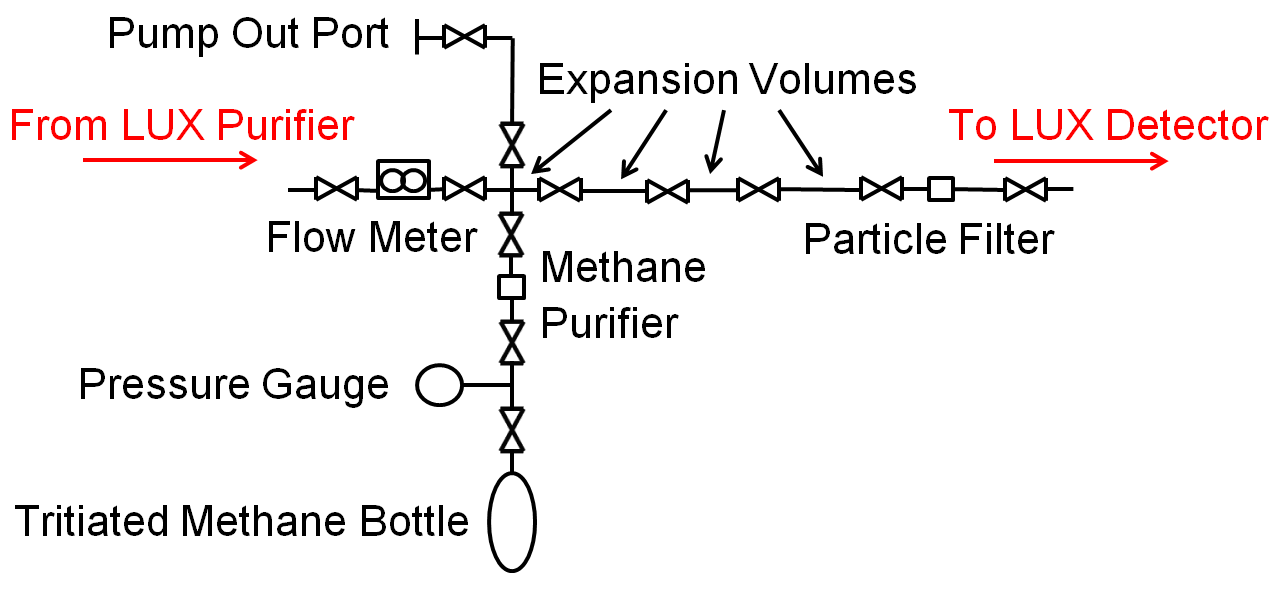
\includegraphics[width=80mm]{fig/TritiumPlumbing.png}
\caption{Plumbing diagram of the CH$_3$T injection system for LUX. CH$_3$T is injected downstream of the xenon gas purifier so that it passes through the detector prior to being removed.  Red arrows indicate the direction of flow.}
\label{fig:plumbing}
\end{figure}

The CH$_3$T appears in the TPC within minutes of the injection, and is removed via the normal action of the LUX xenon purification system, which operates without interruption during the entire procedure. Its centerpiece is a hot zirconium getter (SAES model PS4-MT15-R1\cite{seas}) that acts upon gaseous xenon and continuously removes all non-noble species including methane. The xenon gas flow is driven by a diaphragm pump at a rate of $\sim$27 standard liters per minute. 

Prior to the first injection of CH$_3$T activity, we first confirmed that the LUX getter unit was capable of efficient methane removal by injecting  $\sim$1 ppm (part-per-million g/g) of natural methane (CH$_4$) into LUX. As shown in Fig.~\ref{fig:ch4_removal}, the CH$_4$ concentration in the gas, monitored with a mass spectrometer, was observed  to decrease exponentially with a time constant of 5.9 $\pm 0.07$ hours. The one-pass efficiency of the getter for CH$_4$ removal was measured to be 97\% under the LUX flow and temperature conditions by sampling the gas before and after the getter. 

On August 8, 2013, an initial injection of 20 mBq of CH$_3$T was performed, followed five days later by an injection of 800 mBq. The count rate of fiducial single-scatter events with S1 $<$ 150 photons detected (phd) (roughly the endpoint of the tritium beta spectrum) is shown in Fig.~\ref{fig:ch3t_removal}. The CH$_3$T activity is clearly observed, with the count rate reaching its maximal value in one hour. For both injections the activity was removed with a six-hour exponential time constant similar to that observed in the CH$_4$ injection. It is worth noting that the observed purification time constant is considerably shorter than the xenon mass turn-over time of LUX (about 40 hours for 370 kg of xenon).  The origin of the short purification time remains under investigation. The location of the CH$_3$T events from the first injection after all corrections is shown in Fig.~\ref{fig:event_location}. As expected, the events are uniform within the detector volume.� An empirical model that describes the removal of CH$_3$T from LUX is presented in Appendix~\ref{sec:appendix2}.

\begin{figure}[h!]
<<<<<<< HEAD
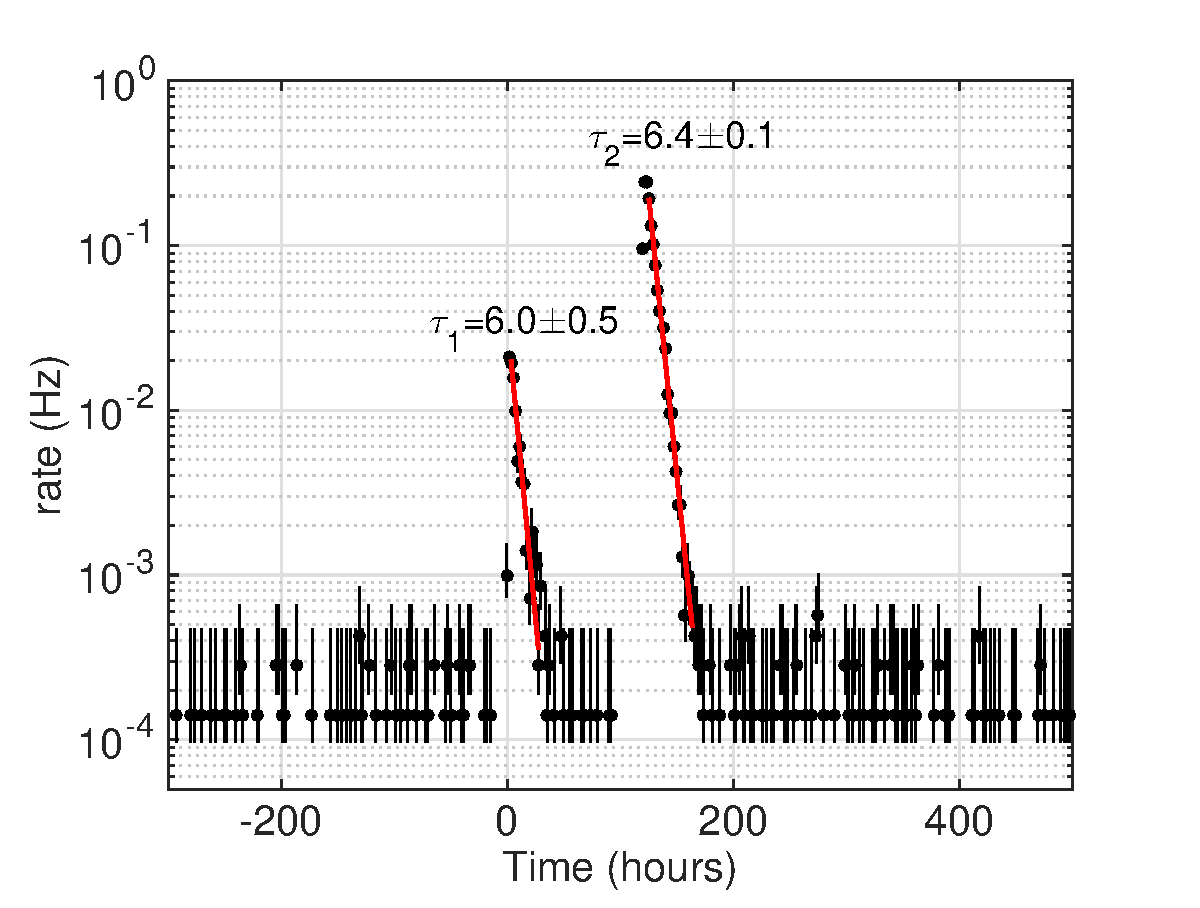
\includegraphics[width=90mm]{fig/CH3T_Rate.eps}
\caption{Rate of single scatter events with S1 below 150 phd in the fiducial volume during the August 2013 CH$_3$T injections.  The magenta and red curves are exponential fits to the activity vs time.}
=======
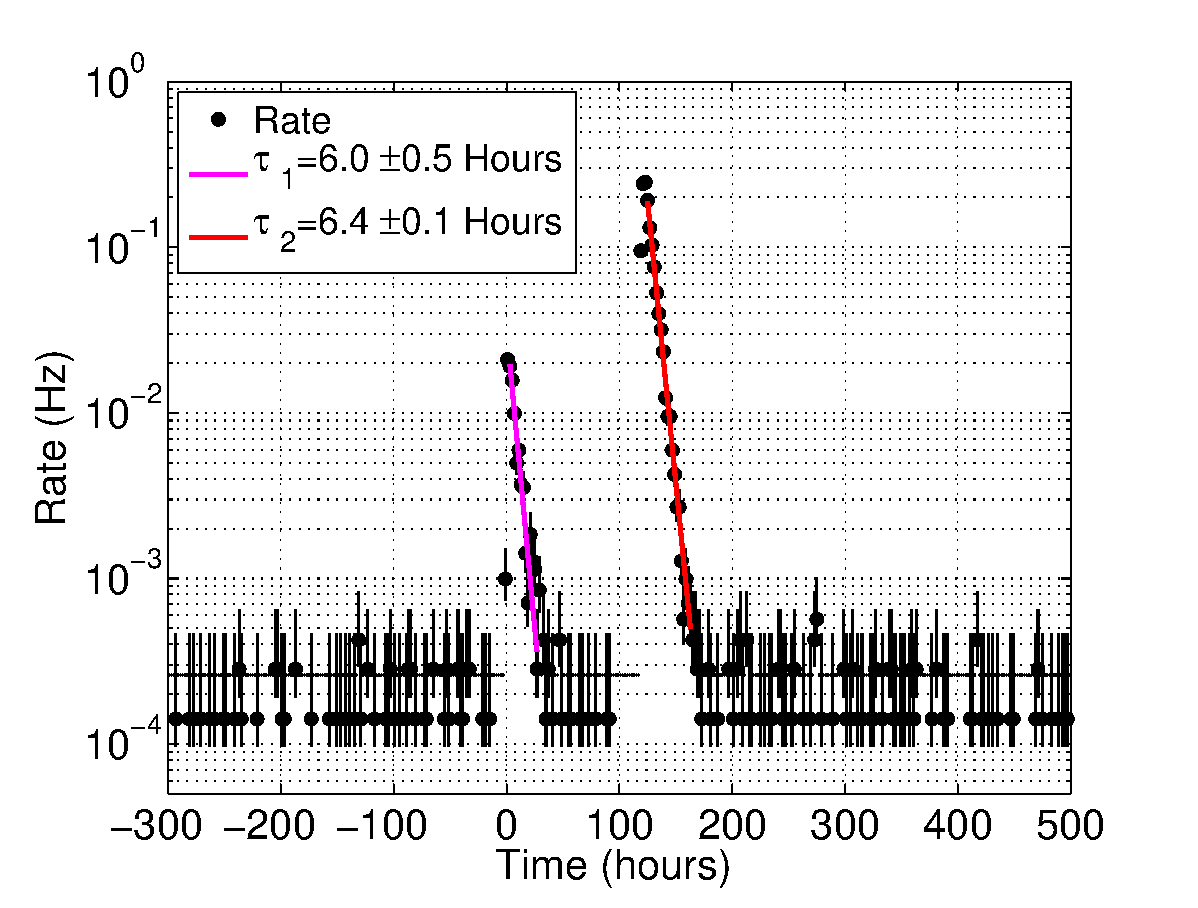
\includegraphics[width=80mm]{fig/CH3T_Rate_fid_150_Run03_Tritium_Rate.eps}
\caption{Rate of single scatter events with S1 below 150 phd in the fiducial volume during the August 2013 CH$_3$T injections.  The magenta and red curves are exponential fits to the activity vs. time.}
>>>>>>> origin/master
\label{fig:ch3t_removal}
\end{figure}


 
\begin{figure}[h!]
<<<<<<< HEAD
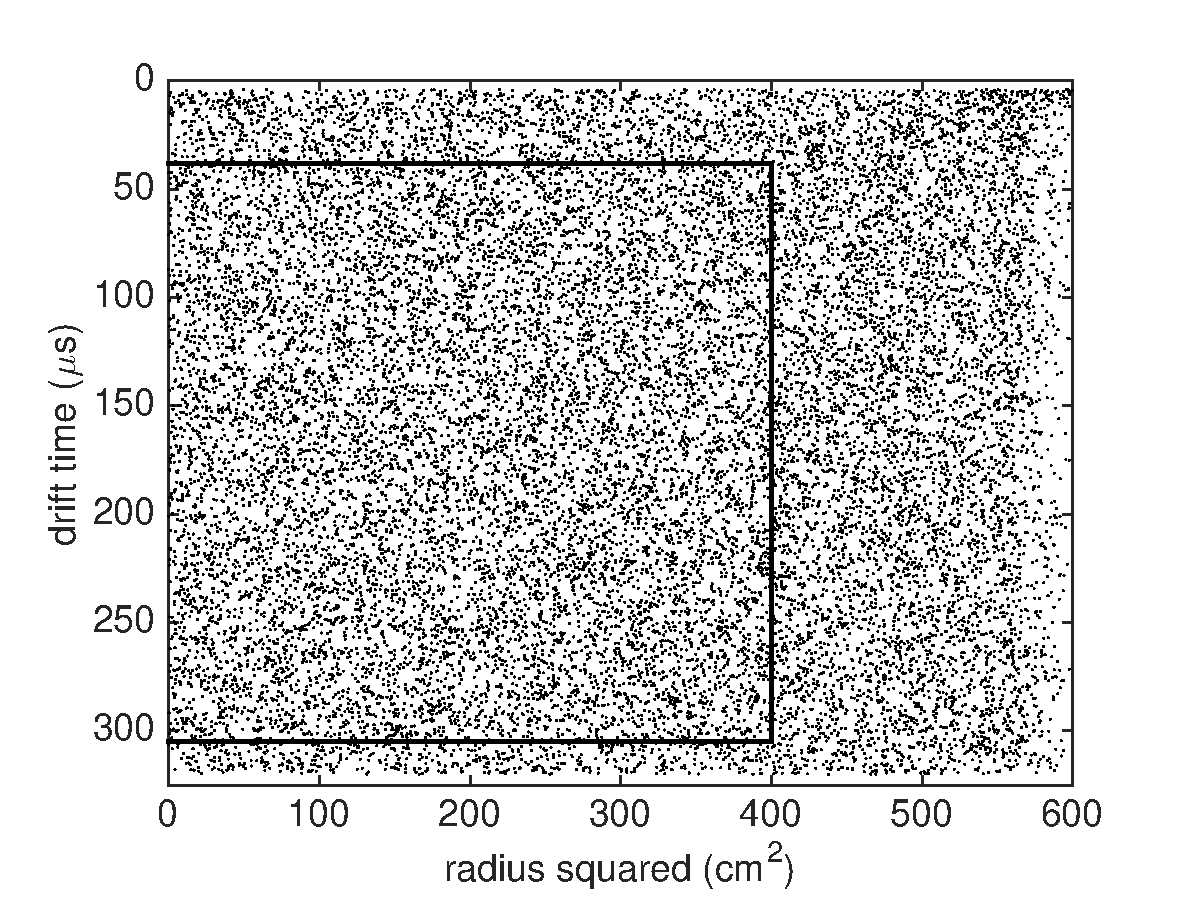
\includegraphics[width=90mm]{fig/rz_scatter.eps}
\caption{The location of events in drift time vs. detector radius squared for the August 2013 CH$_3$T injection. The drift time is a proxy for the $z$ coordinate of the event. The solid black line represents the fiducial volume used in \cite{lux-reanalysis}.}
=======
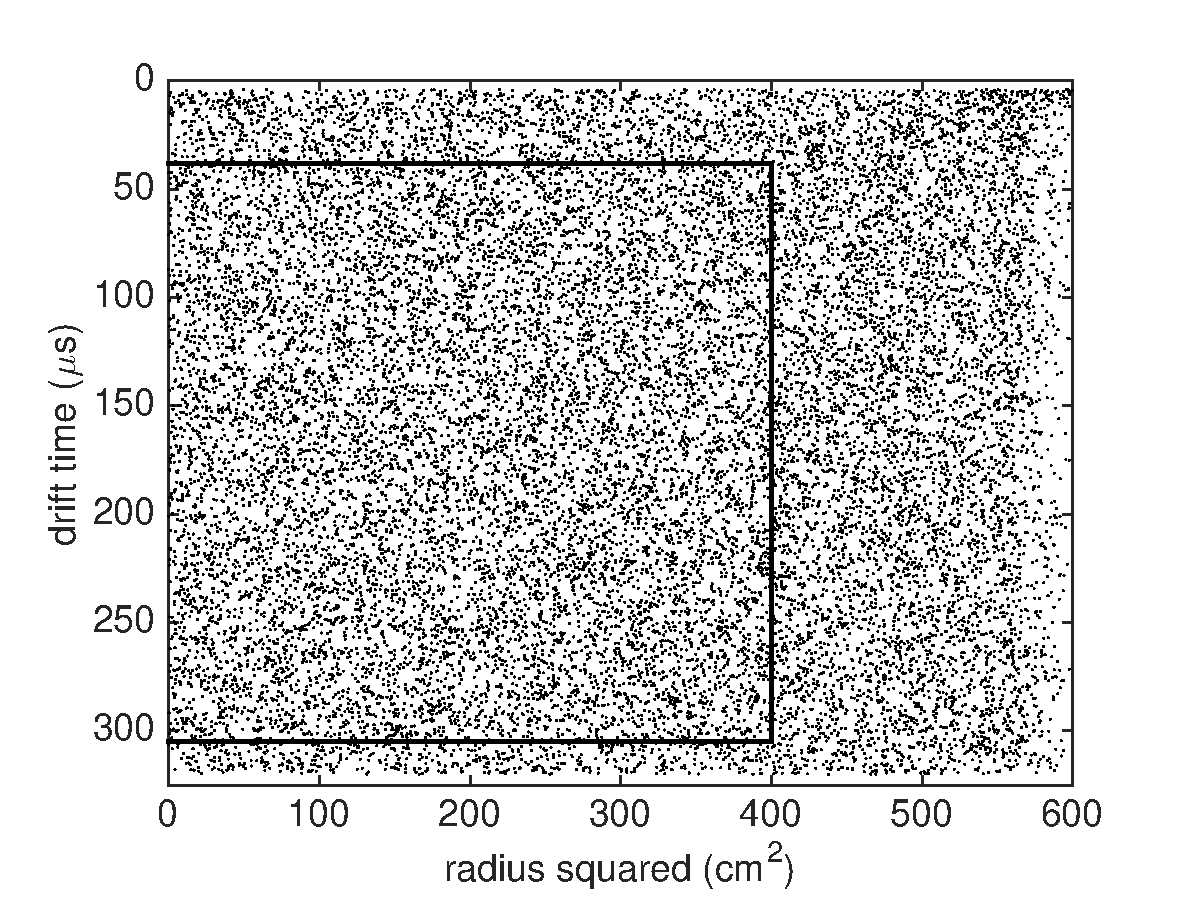
\includegraphics[width=80mm]{fig/rz_scatter.eps}
\caption{The location of events in drift time vs. detector radius squared for the August 2013 CH$_3$T injection. The drift time is a proxy for the $z$ coordinate of the event. The solid black line represents the fiducial volume used in~\cite{lux-reanalysis}.}
>>>>>>> origin/master
\label{fig:event_location}
\end{figure}







\section{Results}

At the conclusion of Run 3, in December of 2013, a total of 10 Bq of tritium was injected into LUX and removed. A total 325,000 events were observed in the active volume of LUX, of which 183,000 events were in the fiducial volume at the nominal LUX electric field of 180 V/cm. Another 4,500 fiducial events were collected in a special run at a reduced field of 105 V/cm. We correct the S1 and S2 signals for spatial effects such as the light collection efficiency and the free electron lifetime with $\rm ^{83m}$Kr data as described in \cite{lux-reanalysis}. 


We interpret the data in terms of the combined energy model for electron recoils \cite{Platzman}, where the total energy of an event is directly proportional to the number of quanta produced (electrons plus scintillation photons):

\begin{equation}
\rm E_{total} = W \cdot (n_{\gamma} + n_e )
\label{platzman_eq}
\end{equation}

\noindent
where $\rm E_{total}$ is the energy of the deposition in keV and  $\rm n_\gamma$ and $\rm n_e$ are the number of photons and electrons respectively. We use a $W$ value of 13.7 $\rm \pm$ 0.2 eV/quanta \cite{Dahl_Thesis}. In LUX $n_{\gamma}$ and $n_e$ are proportional to the S1 and S2 signals, with gain factors $g_1$ and $g_2$: 
%We use a $W$ value of 13.7 $\rm \pm$ 0.2 eV/quanta \cite{Dahl_Thesis}. In LUX $n_{\gamma}$ and $n_e$ are proportional to the S1 and S2 signals, with gain factors $g_1$ and $g_2$:

\begin{equation}
\rm E_{total} = W \cdot \left(\frac{S1}{g_1} + \frac{S2}{g_2} \right)
\label{energy_eq}
\end{equation}

\noindent
where S1 and S2 have units of photons detected (phd) and $g_1$ and $g_2$ have units of phd per quanta. $g_1$ is the average light collection efficiency times the average quantum efficiency of the PMT arrays, while $g_2$ is the product of the electron extraction efficiency at the liquid-gas surface and the average single electron size in phd. $g_1$ and $g_2$ are measured with line source data in the LUX Run 3 to be $0.120 \pm 0.002$ and \fixit{This is the eee, not g2: $0.431 \pm 0.015$}\cite{lux-reanalysis, lux-prd}. For the December 2013 tritium calibration presented here, the gains g1 and g2 are constrained by optimizing the combined energy model to the true tritium spectral shape \cite{Tritium_Eq_Simpson} convolved with detector resolution. We find values of $g_1$ = \gone  ~and  $g_2$ = \gtwo.  The difference between these values with those quoted in Ref. \cite{lux-reanalysis, lux-prd} is taken as a systematic error for the results present in Ref. \cite{lux-reanalysis, lux-prd}.

\begin{figure}[h!]\centering
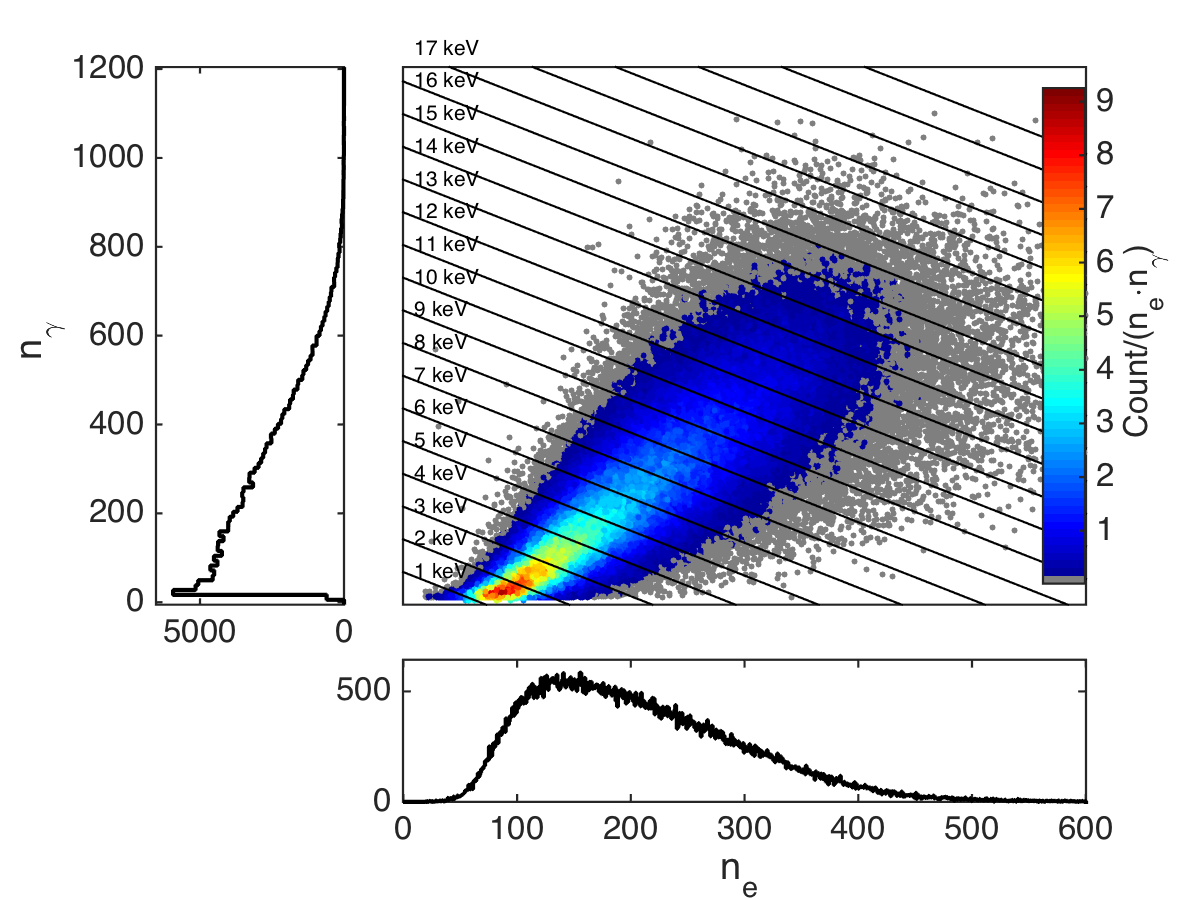
\includegraphics[width=90mm]{fig/tritium_scatter.png}
\caption{Scatter plot of $n_e$ vs $n_{\gamma}$ for 149,000 fiducial tritium events at 180 V/cm. Lines of constant energy are indicated assuming a $W$ value of 13.7 eV/quanta. The data is projected into $n_e$ and $n_{\gamma}$ histograms on each axis.}
\label{fig:tritium-scatter}
\end{figure}


\begin{figure}[h!]
\begin{center}
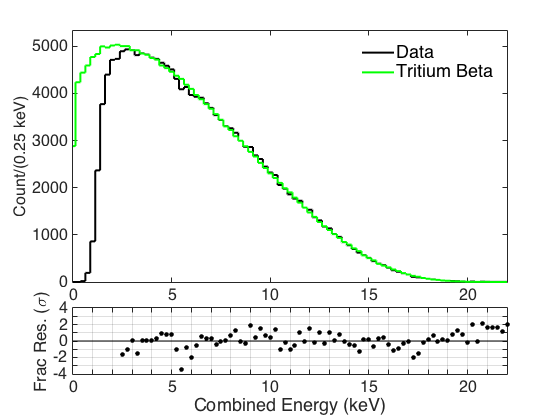
\includegraphics[width=90mm]{fig/tritium-spectrum-linear.png}
\caption{The tritium energy spectrum measured by LUX with the combined energy model (black) compared to several theory models: a pure tritium spectrum (dashed blue), and a tritium spectrum convolved with detector resolution  $\rm \frac{\sigma_E}{W} = \sqrt{\sigma^2(n_{\gamma})+ \sigma^2(n_e)}$. }
\label{fig:tritium-spectrum}
\end{center}
\end{figure}

%S1 ($\rm \sigma(n_{\gamma}))$ and S2 ($\rm \sigma(n_e)$)

A scatter plot of $n_e$ vs $n_{\gamma}$ for the tritium data at 180 V/cm is shown in Fig. \ref{fig:tritium-scatter}, along with the projected histograms on each axis. Contours of constant energy in 1 keV intervals are also plotted, derived from Eq. \ref{platzman_eq}. 


The tritium energy spectrum, obtained by projecting the data along the lines of constant energy, is shown in Fig. \ref{fig:tritium-spectrum}. The data is compared to an ideal tritium spectrum \cite{Tritium_Eq_Simpson}, with no detector effects, and a tritium spectrum with an energy smearing factor of $\rm \frac{\sigma_E}{W} = \sqrt{\sigma(n_{\gamma})^2 + \sigma(n_e)^2}$, where $\rm \sigma(n_{\gamma})$ and $\rm \sigma(n_e)$ represent the detector resolution for photon and electron counting. The ratio of the data to the smeared theoretical spectrum is shown in Fig. \ref{fig:ER-threshold}, along with an empirical fit to an error function. The effective 50\% energy threshold is found to be 1.30 $\pm$ 0.013 keV. The good agreement between data and theory from 2 keV to the endpoint of the tritium spectrum supports the combined energy model in Eq.\ref{platzman_eq}.

\begin{figure}[h!]\centering
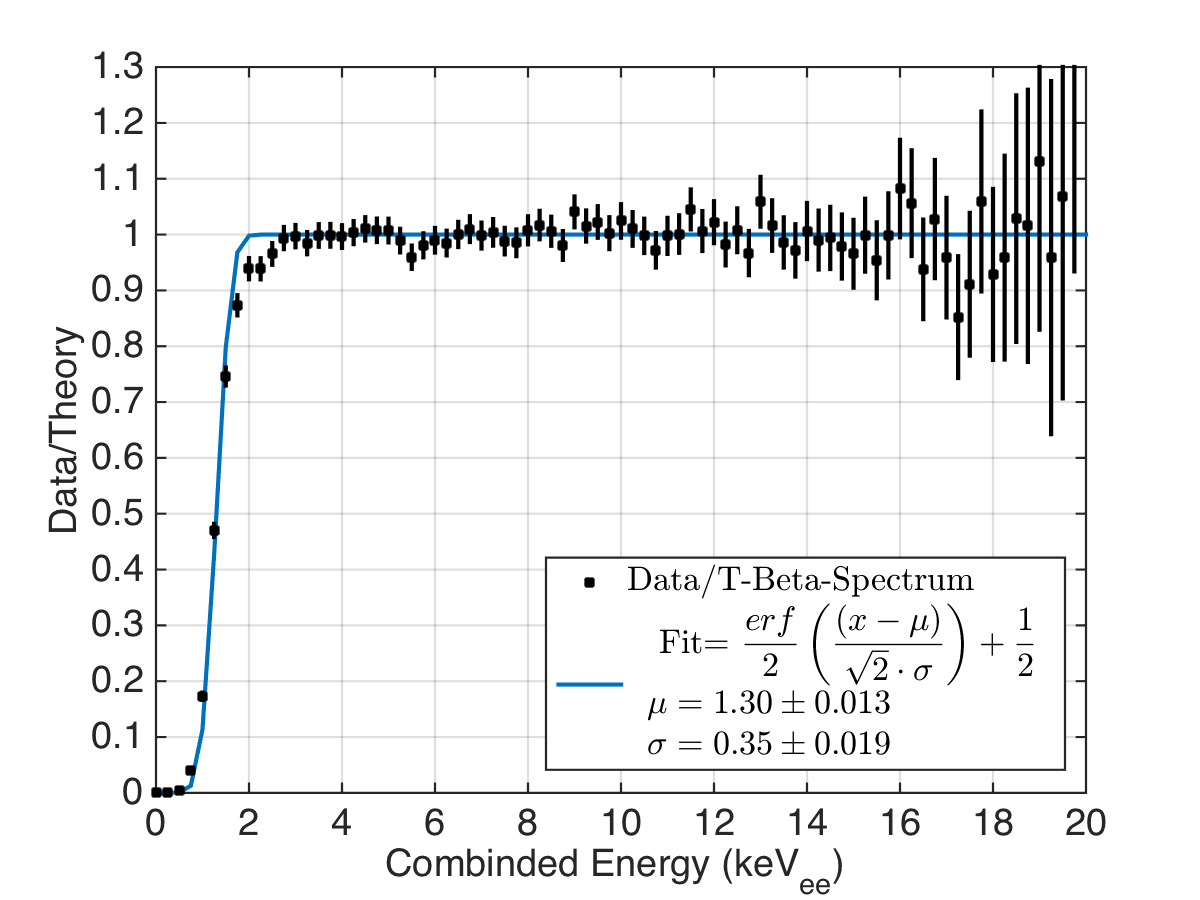
\includegraphics[width=90mm]{fig/E_Thres_Fit.png}
\caption{ER threshold measured by comparing the measured energy spectrum to the smeared tritium spectrum. A fit to an error function is shown.}
\label{fig:ER-threshold}
\end{figure}


%Individual events on the plot are smeared by detector resolution and electron-ion pair recombination fluctuations. Detector resolution is comprised of statistical fluctuations in counting photons and electrons in the S1 and S2 channel. The finite resolution in S1 and S2 smear events along the vertical and horizontal axis, respectively. Recombination fluctuations ($\rm \sigma(R)$) smear events along the contours of constant energy, and thus cancel out in the combined energy model of Eq.\ref{platzman_eq}. 


The mean light and charge yields of ER events in LUX are obtained by dividing the mean light and charge signals by the combined energy in each energy bin. The result is shown for 180 V/cm and 105 V/cm in Fig. \ref{fig:ER-LY-QY} along with NEST v0.98 model predictions at each field \cite{NEST_2013}. For these plots a small correction has been applied to the data to account for smearing of tritium events across energy bins due to the detector's resolution and the spectral shape \cite{Dobi_Thesis}\footnote{We have verified with an internal $^{83m}Kr$ calibration source that the light yield of LXe is unaffected by the presence of CH$_4$ at concentrations up to $\sim$1 part per million. For the CH$_3$T measurements reported here the concentration was ($<$ $\rm10\times10^{-12}$ g/g). }

\begin{figure}[h!]\centering
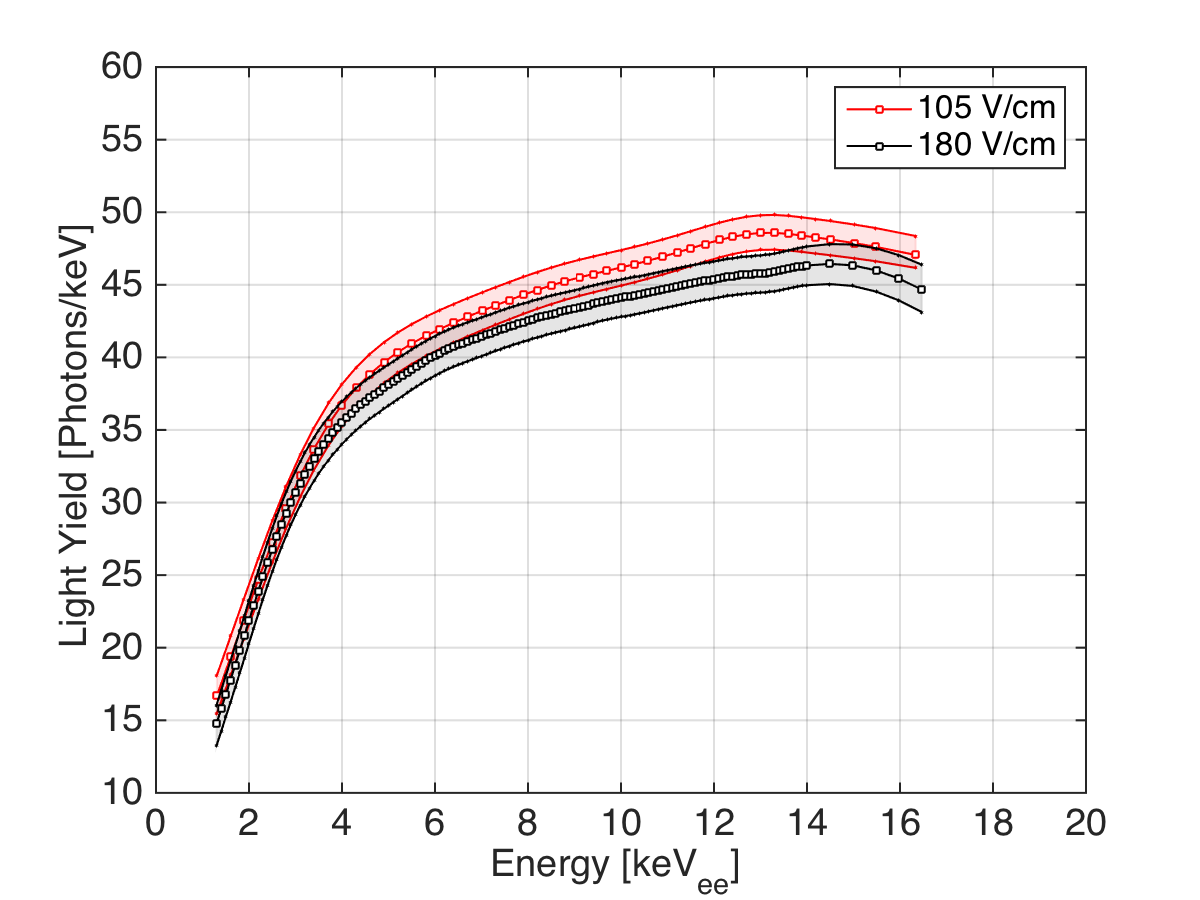
\includegraphics[width=90mm]{fig/ER_LY.png}
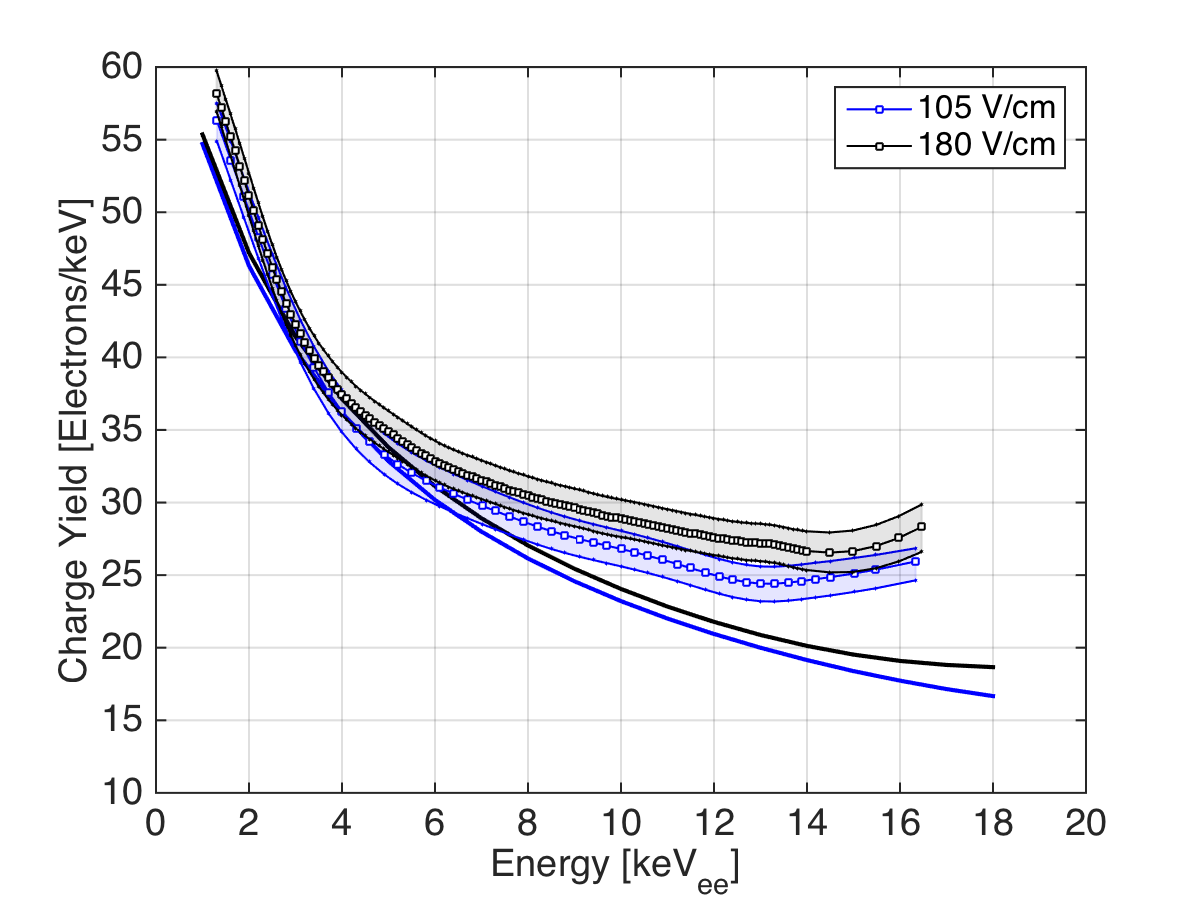
\includegraphics[width=90mm]{fig/ER_QY.png}
\caption{The light yield and charge yield of ER events in LUX at 180 V/cm (black) and 105 V/cm (blue) compared to NEST v0.98 (2013). The bands indicate the systematic errors on $g_1$ and $g_2$, which are fully correlated across all energy bins. $g_1$ is anti-correlated with $g_2$, such that an increase in the charge yield within the grey band must be compensated by an equivalent decrease in the light yield. Upper: Light yield. Lower: the charge yield. The solid lines represent the NEST model predictions at each field \cite{NEST_2013}.}
\label{fig:ER-LY-QY}
\end{figure}

The light yield measurements are compared to similar measurements by other authors in Fig. \ref{fig:Re_LY}. To remove detector effects from this comparison, the light yield is normalized to the yield of the 32.1 keV electron capture decay of $\rm ^{83m}Kr$ at zero electric field. For LUX this light yield is measured to be $\rm 63.8 \pm 3$ $\rm n_\gamma$/keV. The findings are consistent with the expectation that the tritium light yields at 105 and 180 V/cm lie between those at zero field and 450 V/cm from \cite{Aprile_LY} and \cite{Baudis}. It is worth noting that Refs. \cite{Aprile_LY} and \cite{Baudis} use Compton scatters as the source of ER events, while in tritium data the ER source is a beta decay. At low energy beta decays and Compton scatters should leave similar track lengths and produce similar event characteristics. The comparison of Fig. \ref{fig:Re_LY} confirms this expectation within the experimental uncertainties.

\begin{figure}[h!]\centering
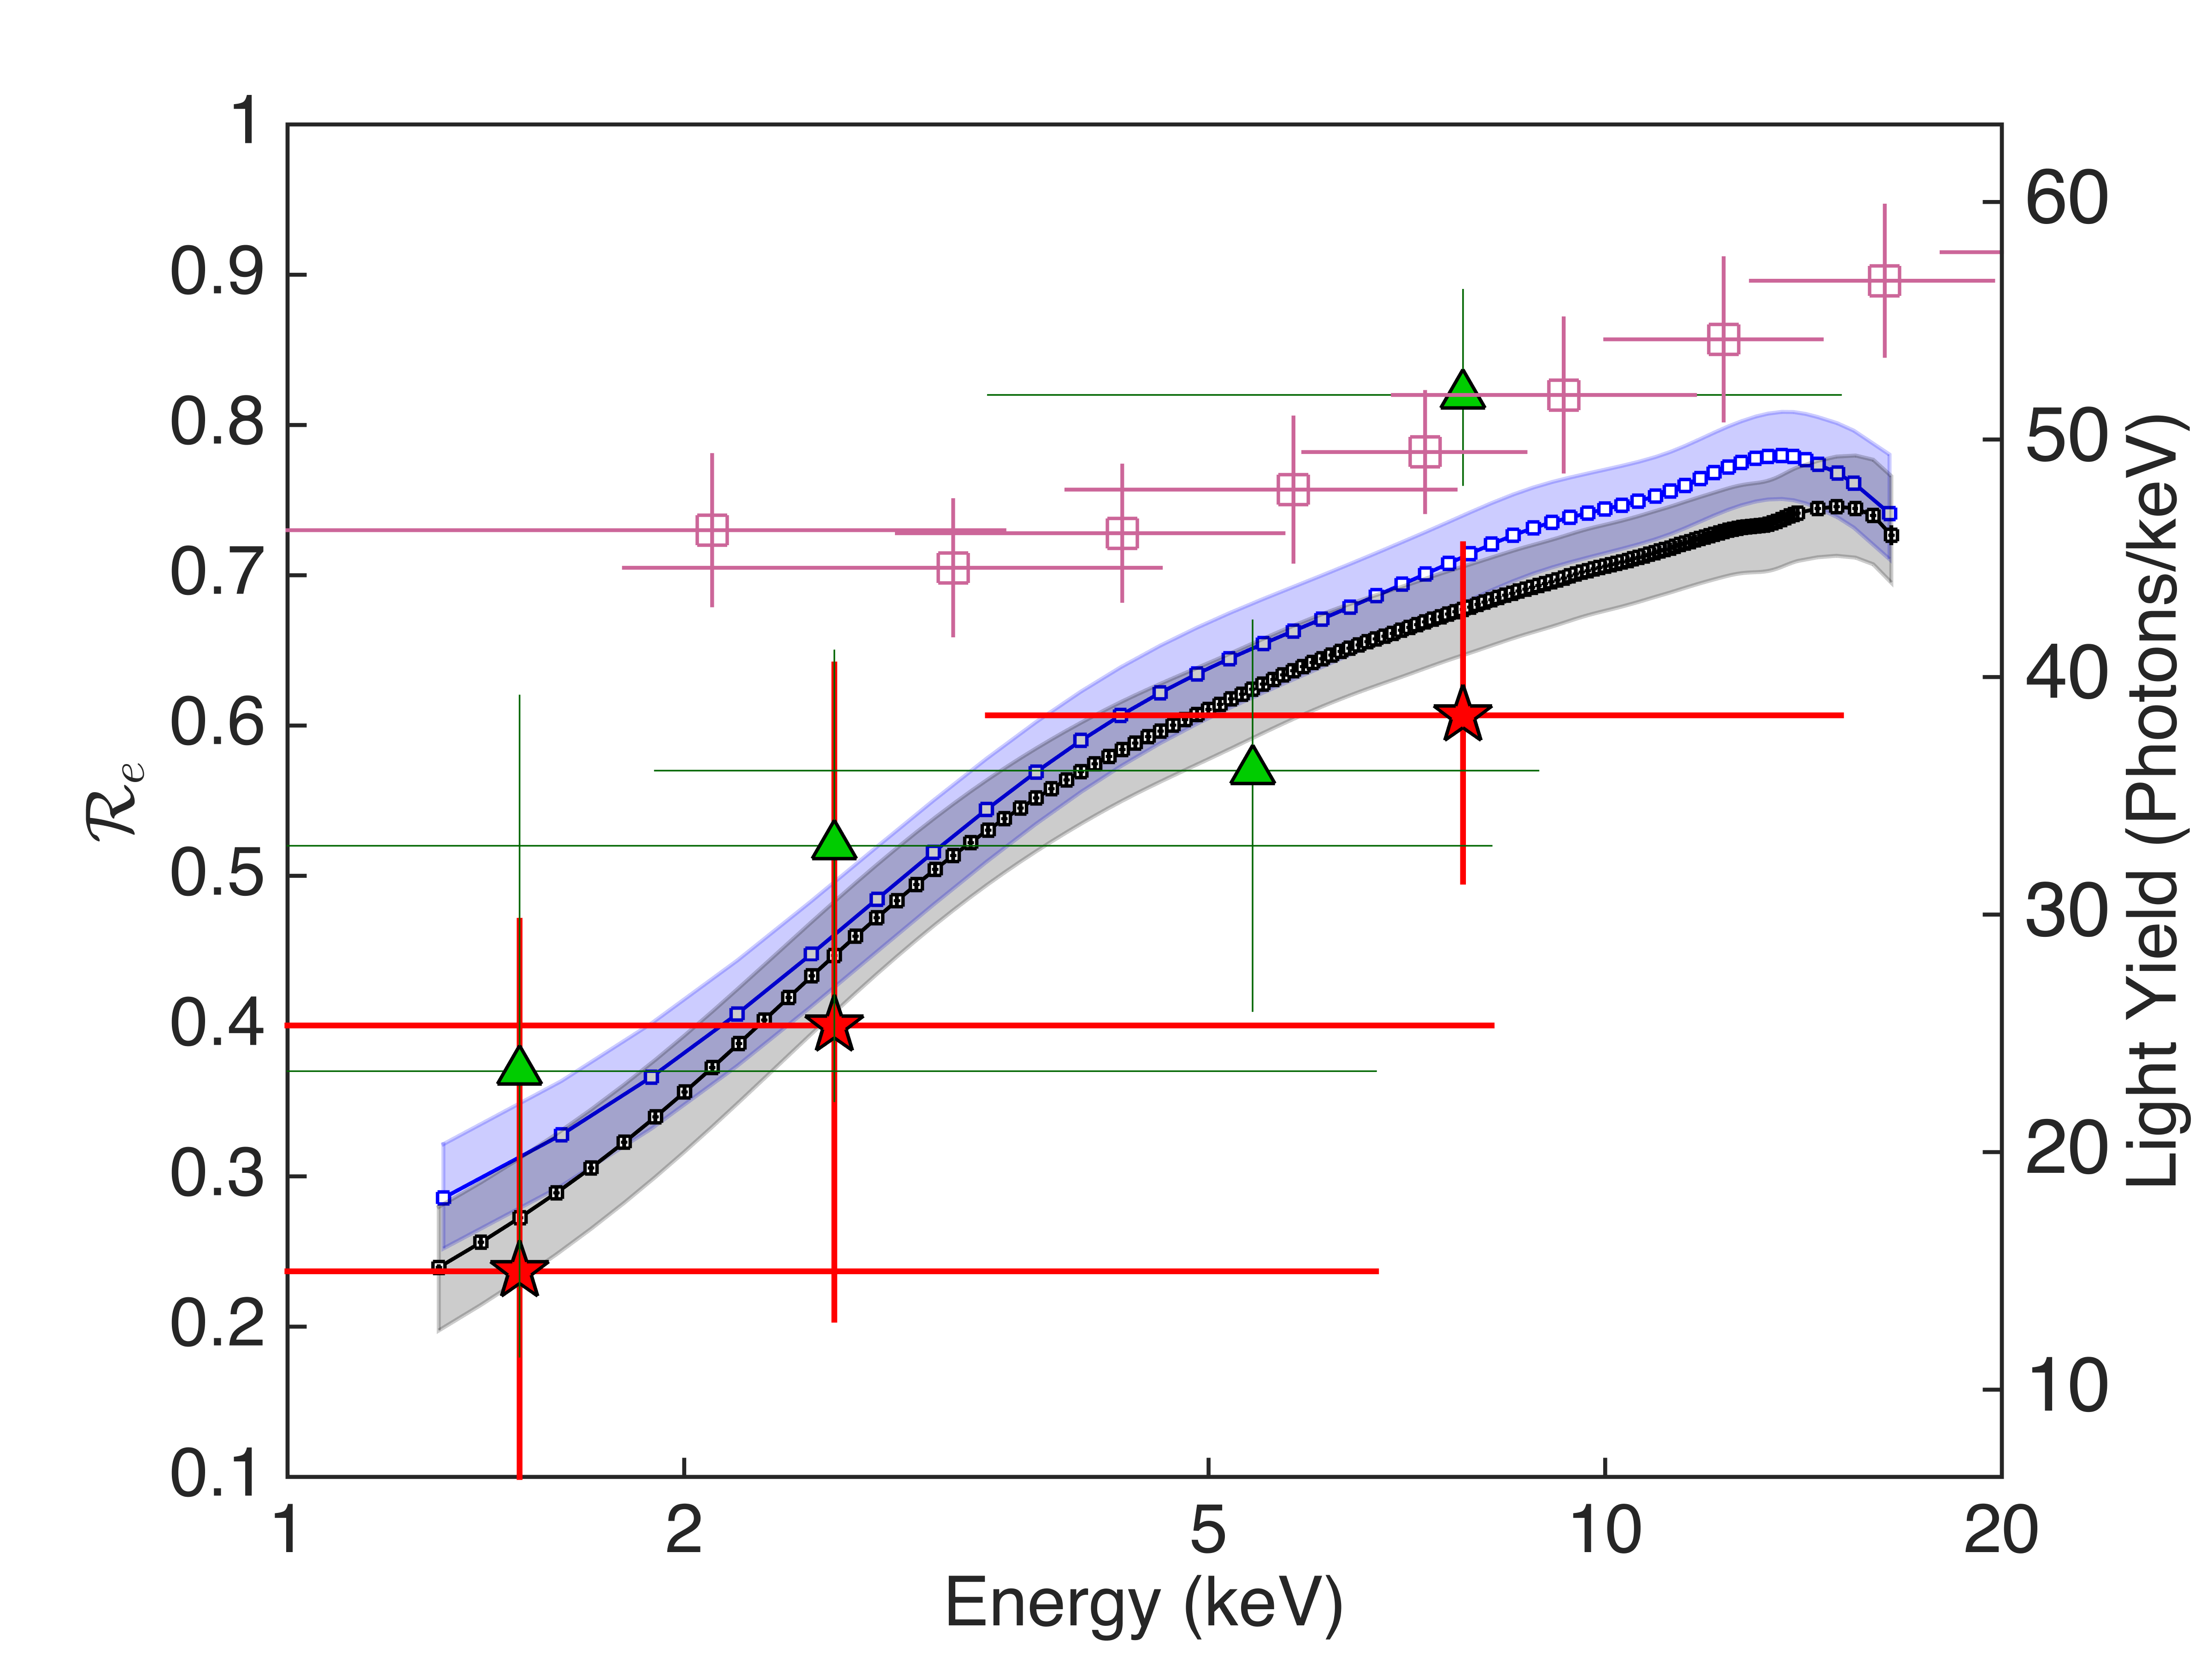
\includegraphics[width=88mm]{fig/Re_LY_log.png}
\caption{Light yield measurement from LUX tritium data compared to results from other authors. Left vertical scale: light yield relative to that of the 32.1 keV decay of $\rm^{83}Kr $ at zero field. Right vertical scale: absolute light yield measurements from LUX tritium data. Shaded blue curve is tritium at 105 [V/cm], shaded black curve is tritium at 180 [V/cm]. Magenta squares represent zero field measurements from \cite{Aprile_LY}. Cyan triangles and red circles represent a Compton scattering measurement at zero field and 450 [V/cm] from \cite{Baudis}. }
\label{fig:Re_LY}
\end{figure}


As shown in Fig. \ref{fig:ER-LY-QY}, we find that the light yield increases rapidly from 1 and 6 keV, and then becomes mostly energy independent over the remainder of the tritium spectrum. The charge yield exhibits the complimentary behavior as expected from the combined energy model. These effects can also be illustrated by plotting the number of photons and electrons as a function of energy, as shown in Fig. \ref{fig:quanta-vs-energy}. Also shown in Fig. \ref{fig:quanta-vs-energy} are the total number of quanta assuming a $W$ value of 13.7 eV/quanta (black), and the initial number of ions (violet) and excitons (cyan) prior to recombination, where we assume an exciton-to-ion ratio of 0.2 \cite{alpha-value} independent of energy. Under this assumption we interpret the charge yield data as a measure the recombination fraction at each energy according to

\begin{equation}
r = \frac{\frac{n_{\gamma}}{n_e} - \alpha}{\frac{n_{\gamma}}{n_e} + 1}
\end{equation}

\noindent
where $r$ is the recombination fraction and $\alpha$ is the initial exciton-to-ion ratio. The implied recombination fraction as a function of energy is shown in Fig. \ref{fig:recombination}. Here the falling charge yield and rising light yield between 1 and 6 keV appears as a rapid rise in the recombination fraction with increasing energy. 

\begin{figure}[h!]\centering
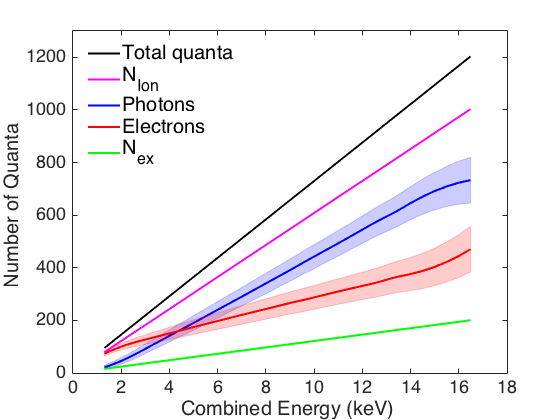
\includegraphics[width=90mm]{fig/quanta-vs-energy.png}
\caption{Top: The mean number of electrons (red) and scintillation photons (blue) produced in LUX at 180 V/cm as a function of energy. The bands indicate the correlated systematic errors on $g_1$ and $g_2$. Also shown are the total number of quanta, primary ions, and primary excitons, assuming an exciton to ion ratio of 0.2. }
\label{fig:quanta-vs-energy}
\end{figure}

\begin{figure}[h!]\centering
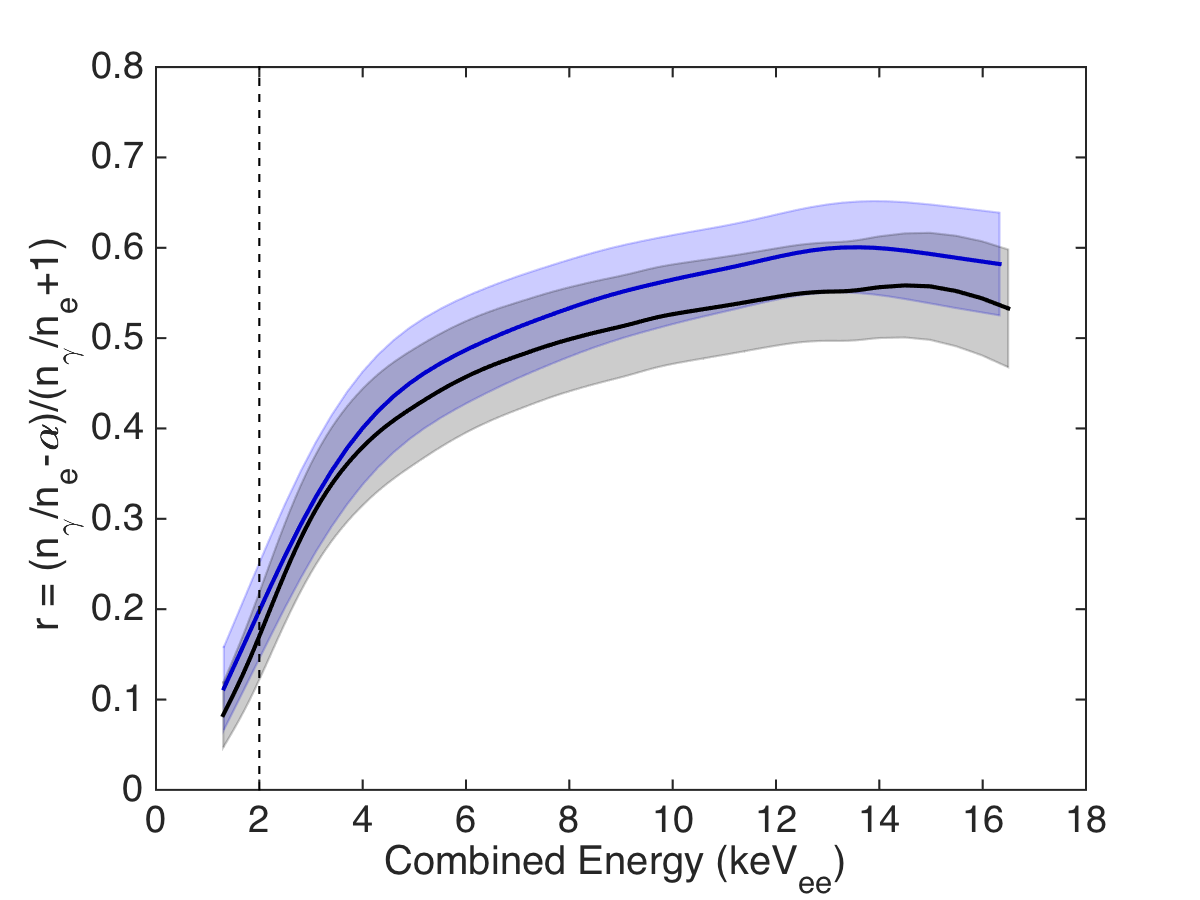
\includegraphics[width=90mm]{fig/recombination.png}
\caption{Recombination fraction of ER events at 180 V/cm (black) and 105 V/cm (blue), assuming an exciton-to-ion ratio of 0.2.}
\label{fig:recombination}
\end{figure}

\begin{figure}[h!]\centering
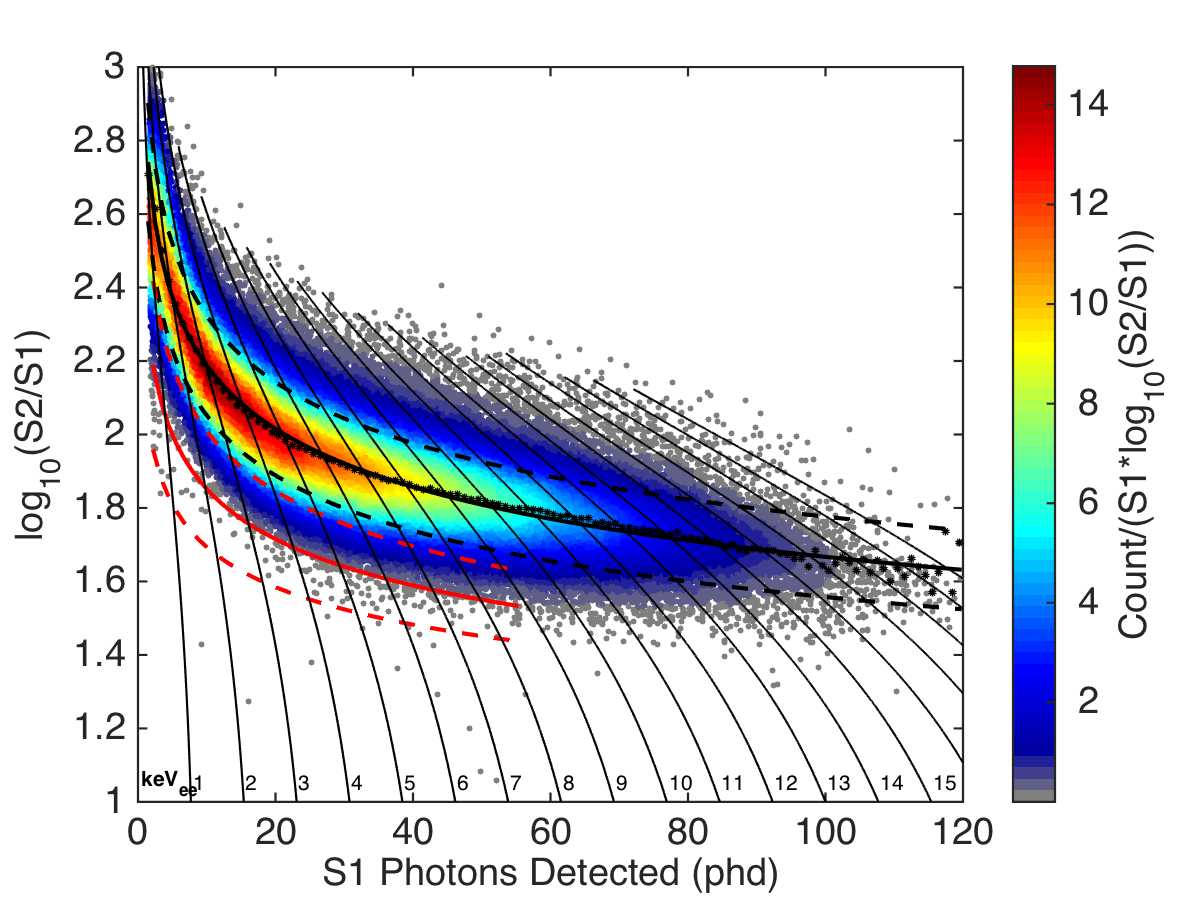
\includegraphics[width=90mm]{fig/CH3T_ER_Band.png}
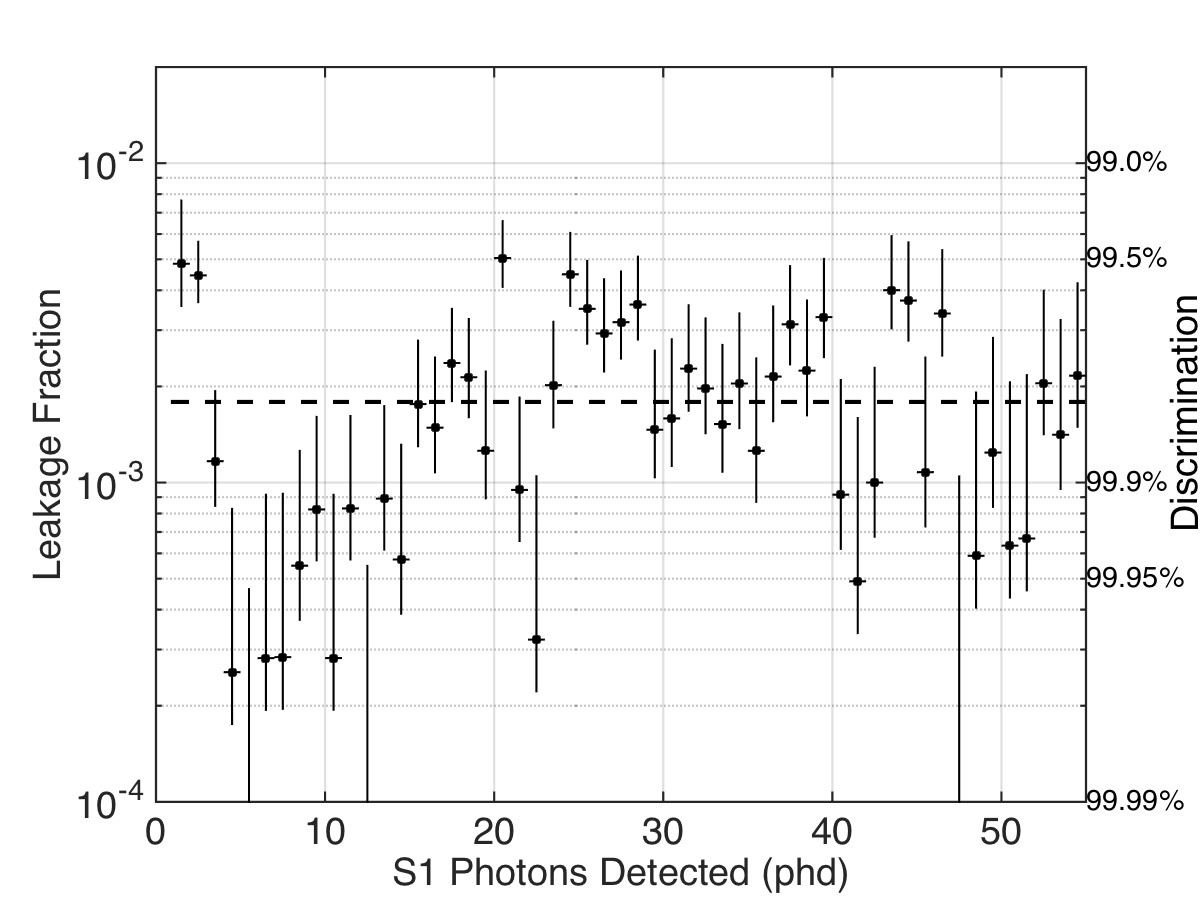
\includegraphics[width=85mm]{fig/CH3T_Leakage_Run03.png}
\caption{Top: The electron recoil band of LUX illuminated by 130,000 tritium events at the nominal LUX electric field of 180 V/cm.  The recoil discriminant variable, log(S2/S1), is shown vs. S1 between 1 and 50 phd in S1 (about $\rm1-8 keV_{ee}$). Also indicated in black are the mean and the 10\% and 90\% contours. The solid red line represents the mean NR band determined with DD neutron generator data. The dashed red indicates the 10\% and 90\% contours of the NR band. Bottom: LUX recoil discrimination vs. S1. Y-axis labels: left -  leakage fraction ($f$); right - discrimination ($1-f$).}
\label{fig:ER_band}
\end{figure}

%\begin{figure}[h!]\centering
%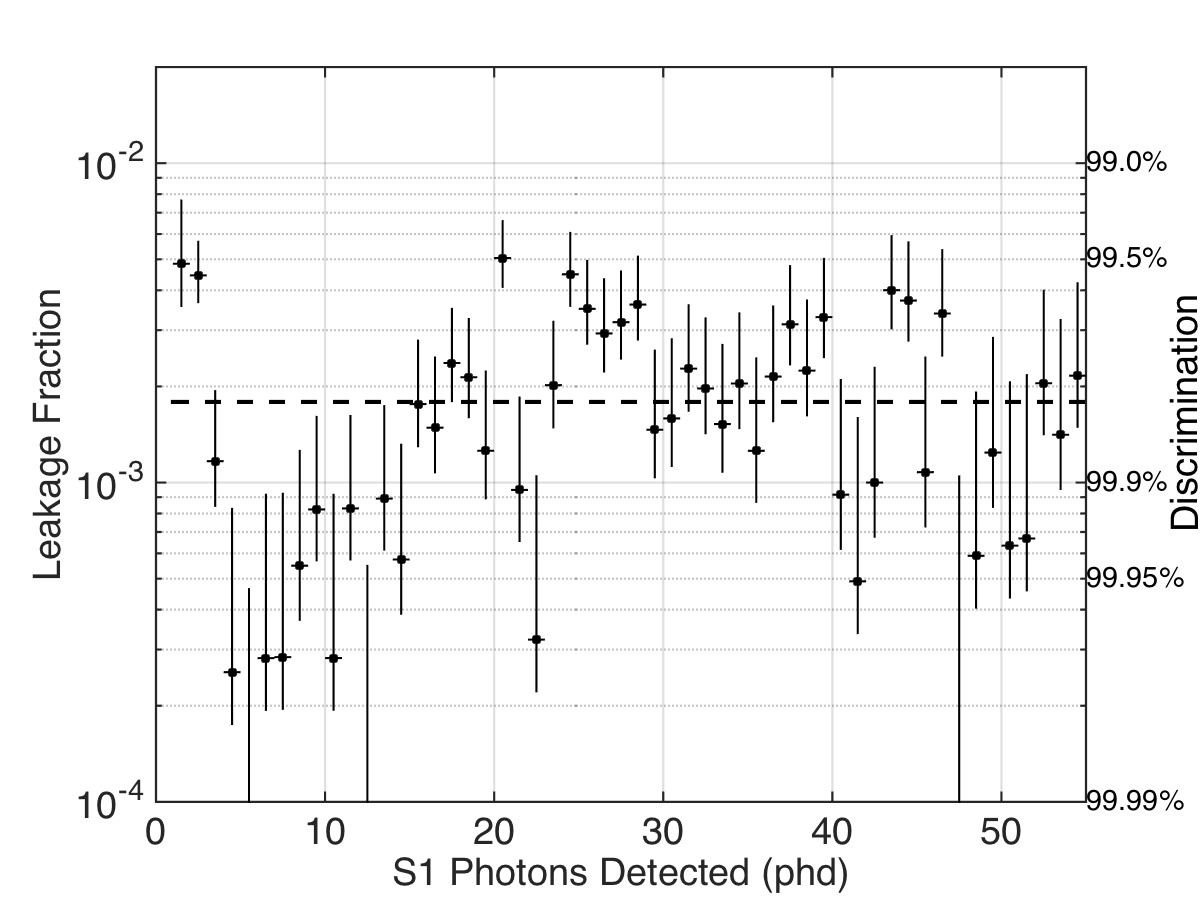
\includegraphics[width=90mm]{fig/CH3T_Leakage_Run03.png}
%\caption{LUX recoil discrimination vs. S1, determined from Fig. \ref{fig:ER_band}. Y-axis labels: left -  leakage fraction ($f$); right - discrimination ($1-f$).}
%\label{fig:Leak}
%\end{figure}



The LUX ER band is shown as log$_{10}$(S2/S1) vs S1 in Fig. \ref{fig:ER_band}(top).  Also shown is the LUX NR band measured with neutron generator data\cite{DD-paper,lux-reanalysis}. The ER band has a characteristic rise at decreasing values of S1 which reflects the increasing charge yield and decreasing light yield below $\sim$6 keVee. The leakage fraction ($f$), defined as the fraction of ER events that fall below the mean of the NR band, is shown in Fig. \ref{fig:ER_band}(bottom) as a function of S1. The recoil discrimination ($1-f$) has an average value of \fixit{99.8\%} for events with S1 between 1 and 50 phd.


\onecolumngrid
\break
\begin{sidewaysfigure}[p!]\centering
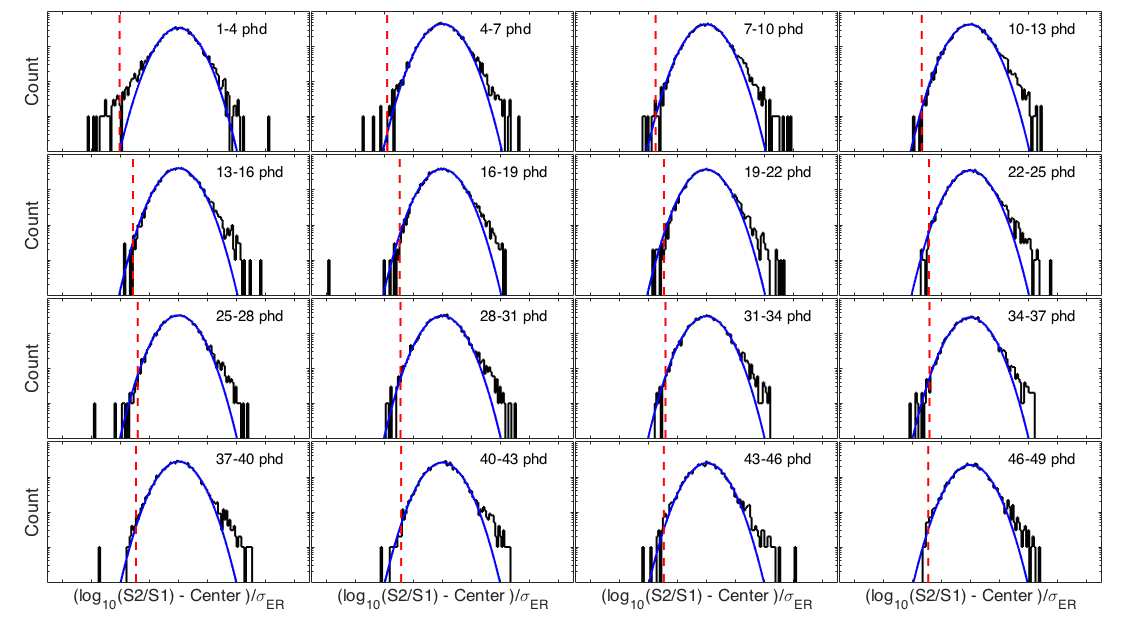
\includegraphics[width=220mm]{fig/Gaussianity/GaussER_all.png}
\caption{Electron recoil population from tritium event about the centroid of the mean in 3 phd bins over the WIMP search region. The red dashed line represents the mean of the NR band in each bin. We observe non Gaussian behavior below three sigma of the ER band and two sigma above. The non Gaussian behavior above the mean of the ER band may be due to the 48\% extraction efficiency.  }
\label{fig:ER-Gauss}
\end{sidewaysfigure}
\twocolumngrid

In Fig. \ref{fig:ER-Gauss} we histogram $\rm log_{10}(S2/S1)$ in bins of S1 with a bin-width of 3 phd. In each bin we show a Gaussian fit to the data after subtracting the centroid and dividing by the Gaussian width. We find that the Gaussian fits describe the data well out to about $2\sigma$ on the upper side and $3\sigma$ on the lower side, beyond which non-Gaussian tails are visible. Only four non-tritium events are expected to be present in these plots out of 180,000 events total, indicating that the small non-Gaussian tails are a genuine feature of ER events in LUX.

In general the width of the ER band should be comprised of three components: the uncertainties on  $\rm n_{\gamma}$ and $\rm n_e$  due to detector resolution ($\rm \sigma(n_{\gamma})$ and $\rm \sigma(n_e)$), and true event-to-event variations in recombination ($\rm \sigma(R)$). $\rm \sigma(n_{\gamma})$ and $\rm \sigma(n_e)$ are responsible for fluctuations in the vertical  and horizontal directions in Fig. \ref{fig:tritium-scatter},  while 
$\rm \sigma(R)$ causes fluctuations along the diagonal lines of constant energy. $\rm \sigma(n_{\gamma})$ and $\rm \sigma(n_e)$ can be measured as a function of energy and are shown in Fig. \ref{fig:recomb-flucs} for LUX tritium data at 180 V/cm\cite{Dobi_Thesis}. Also shown in Fig. \ref{fig:recomb-flucs} is the extracted value of $\rm \sigma(R)$ as a function of energy after controlling for $\rm \sigma(n_{\gamma})$ and $\rm \sigma(n_e)$ by a method described in Ref. \cite{Dobi_Thesis}. 

\begin{figure}[h!]\centering
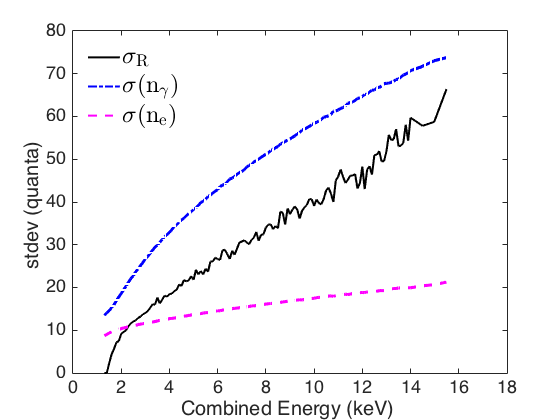
\includegraphics[width=90mm]{fig/recomb_flucs.png}
\caption{Black: recombination fluctuations in LXe measured with LUX tritium data at 180 V/cm. Dot-dash blue: Detector resolution for counting photons. Dashed magenta: Detector resolution for counting electrons.}
\label{fig:recomb-flucs}
\end{figure}

We find that at 180 V/cm in LUX, $\rm \sigma(n_{\gamma})$ is the most important contributor to the ER band width over the entire tritium energy spectrum. Between 2 keVee and 6 keVee, where the WIMP search is most sensitive, $\rm \sigma(n_e)$ and $\rm \sigma(R)$ are of comparable magnitude and secondary importance. We note that an ideal detector would be limited by only $\rm \sigma(R)$.





%Having measured the light and charge yield in-situ we have an understanding of the mean of the electron recoil population for the LUX the WIMP search. To complete the picture we need to understand the variance that lead to the width of the electron recoil band. This is comprise of detector resolution, which is measurable and specific to each detector, and recombination fluctuations. At a given energy the event-to-event standard deviation for the number of recombined ions $\rm \sigma(R)$ is shown in Fig. \ref{fig:recomb-flucs}, extracted using a method outlined in \cite{Dobi_Thesis}. $\rm \sigma(R)$ is a physical property of xenon and produces and irreducible width to the electron recoil band, even with infinite detector resolution. Currently no models exist to predict recombination fluctuations ($\rm \sigma(R)$), thus it is important to measure it in-situ. For the LUX detector conditions we find a linear growth in recombination fluctuations as a function of the number of ions $\rm \sigma(R) = (0.062 \pm 0.005)\cdot N_{ions}$, consistent with the measurement in \cite{Dobi_Thesis}.



%% ER band Gaussianity section. If we want this


%%%%%%%%%%%%%%%%%%%%%%%%%%%%%%%%%%%%%%%%%%%%%%%%%%%%%%%%%%



\section{Summary}

We have characterized the electron recoil band and threshold of the LUX dark matter experiment with a tritium calibration source. The large dataset, high event purity, and simple topology provide a powerful tool to study the detector and to investigate the fundamental properties of LXe as a particle detection medium. The results presented here are used in an improved analysis of the Run 3 WIMP search data in Ref. \cite{lux-reanalysis}.

\appendix

\section{Studies of the removal of CH$_3$T from LXe }
\label{sec:appendix1}

\newcommand*{\Scale}[2][4]{\scalebox{#1}{$#2$}}%

Prior to the first injection of CH$_3$T into LUX, we considered three risks that such a calibration may pose to the dark matter search: 1) that the xenon purification system may be ineffective for CH$_3$T removal; 2) that the interior surfaces of the stainless steel (SS)  gas handling system may become permanently contaminated with CH$_3$T; and 3) that the plastic detector components may outgas unacceptable quantities of CH$_3$T after initial exposure.

To address the first concern we studied the removal of natural methane (CH$_4$) from Xe gas with a heated Zr getter and a mass spectrometer. The purification efficiency was found to be satisfactory\cite{Dobi_CH4}. Furthermore, a test of the completed LUX purification system, including the actual getter unit, was performed several weeks before the first CH$_3$T injection into LUX. In this test $\sim$0.1 grams of CH$_4$ was injected into LUX, and mass spectrometry measurements of the CH$_4$ concentration in the LUX Xe gas were performed over the next several days. The CH$_4$ concentration was observed to decrease exponentially with a time constant of 5.90 $\pm 0.07$ hours as shown in Fig. \ref{fig:ch4_removal}, confirming the effectiveness of the purification system for methane removal.

The behavior of CH$_3$T in SS plumbing was studied in a bench-test with a custom-built Xe gas proportional tube operated at room temperature. Substantial quantities of CH$_3$T activity were injected, counted, and removed from the proportional tube. Initial tests found a small amount of residual activity after purification, however this was resolved by passing the CH$_3$T through a methane purifier (SAES model MC1-905F). No subsequent contamination was observed.

\begin{figure}[h!]\centering
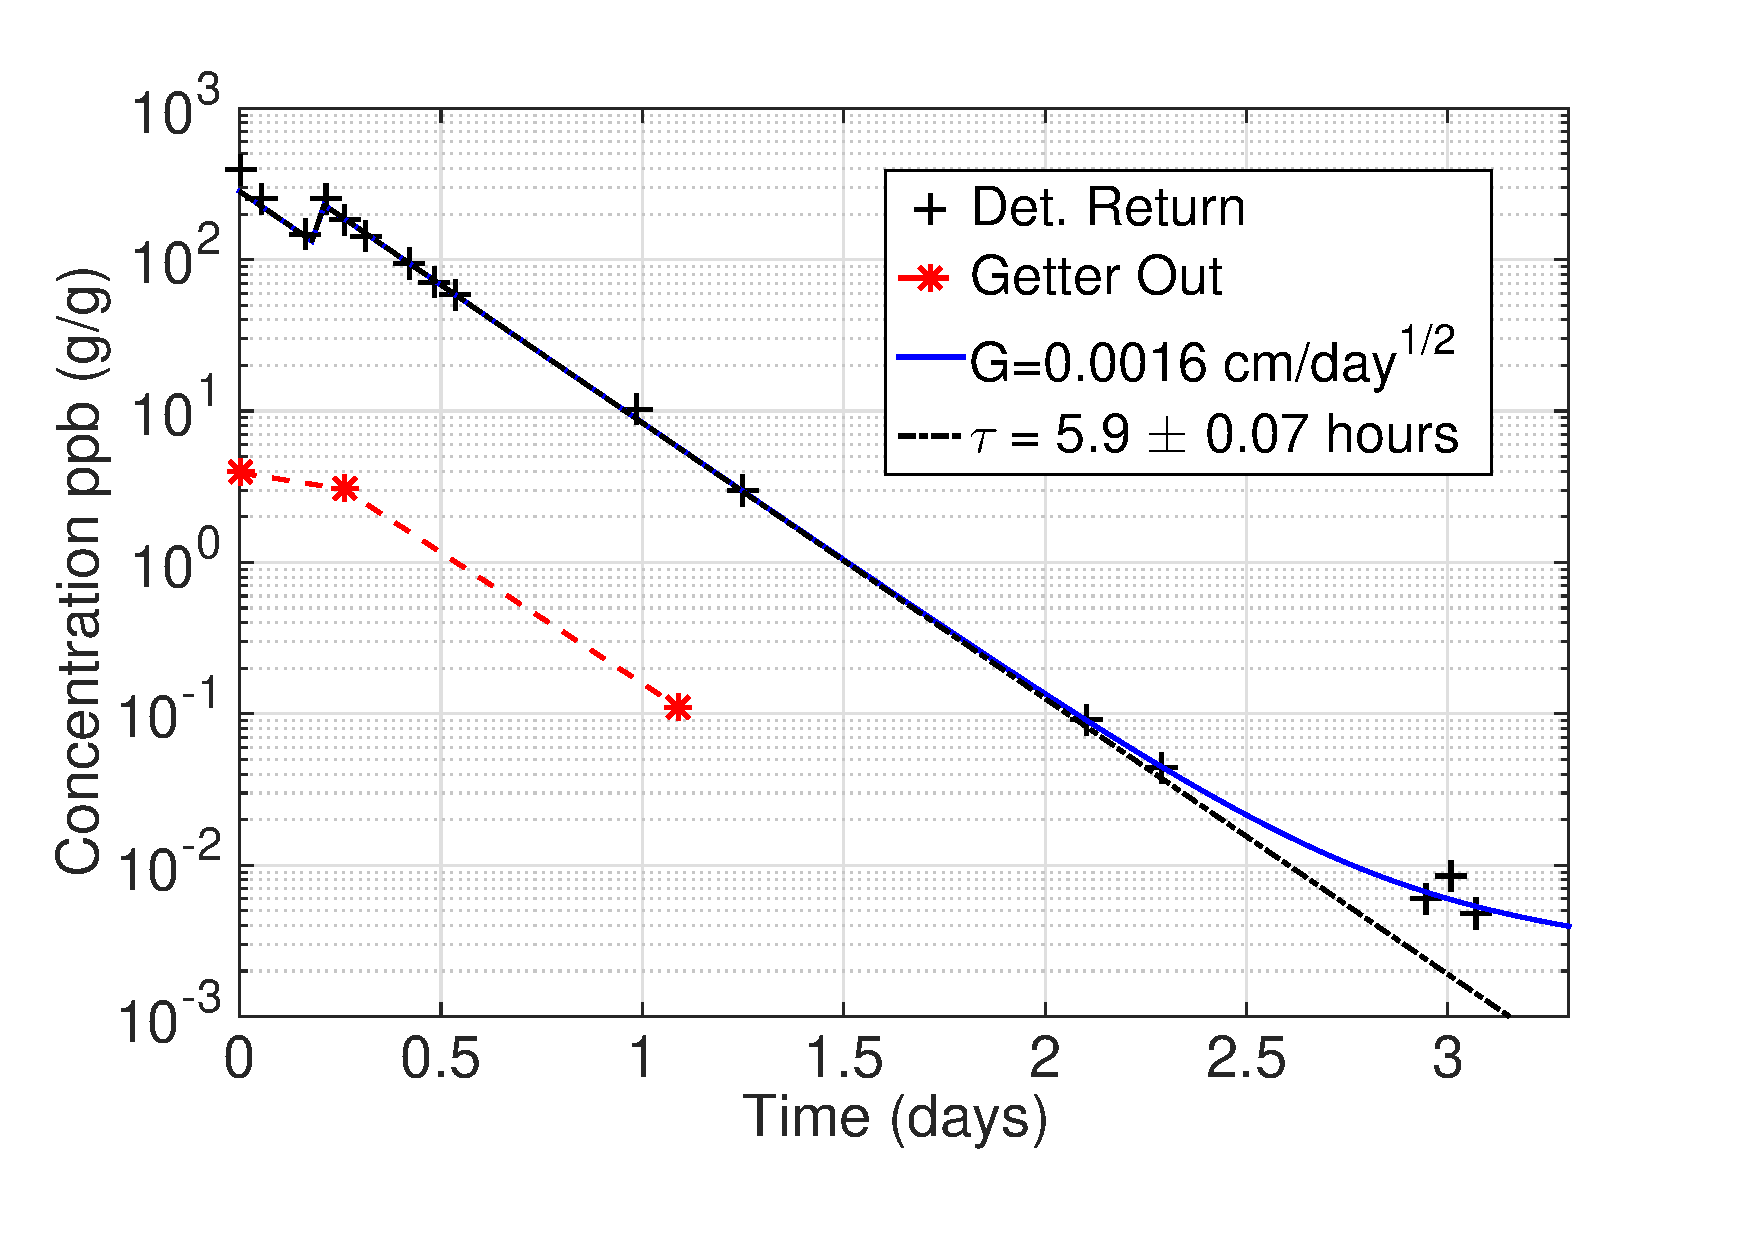
\includegraphics[width=80mm]{fig/July_CH4_wOG.eps}
\caption{Injection and removal of CH$_4$ in LUX prior to the first CH$_3$T injection. CH$_4$ is observed with a gas sampling mass spectrometry system. The black dashed lines shows an exponential fit to the CH$_4$ concentration at the detector return line with a time constant of 5.90 $\pm 0.07$ hours.  The red points indicate measurements at the getter outlet. We find a 97\% one-pass removal efficiency at a flow rate of 27 SLPM. The blue curve shows the upper limit on the effect of outgassing from the plastics. The three data points near t = 3 days are consistent with the limit of detection for methane ($\sim \rm 5\times10^{-3}$ ppb (g/g)) .}
\label{fig:ch4_removal}
\end{figure}

We also performed tests of CH$_3$T injection and removal from LXe with a small detector. One such experiment is shown in Fig. \ref{fig:Density}, where 68,000 Hz of CH$_3$T was injected, counted, and subsequently removed from LXe. Samples of LUX polyethylene and teflon were immersed in the LXe in this experiment, and their outgassing is evident in Fig. \ref{fig:Density}. These data placed constraints on the risk of CH$_3$T outgassing in LUX. In total over one million Hz of CH$_3$T activity was injected and successfully removed in these experiments.

\begin{figure}[h!]\centering
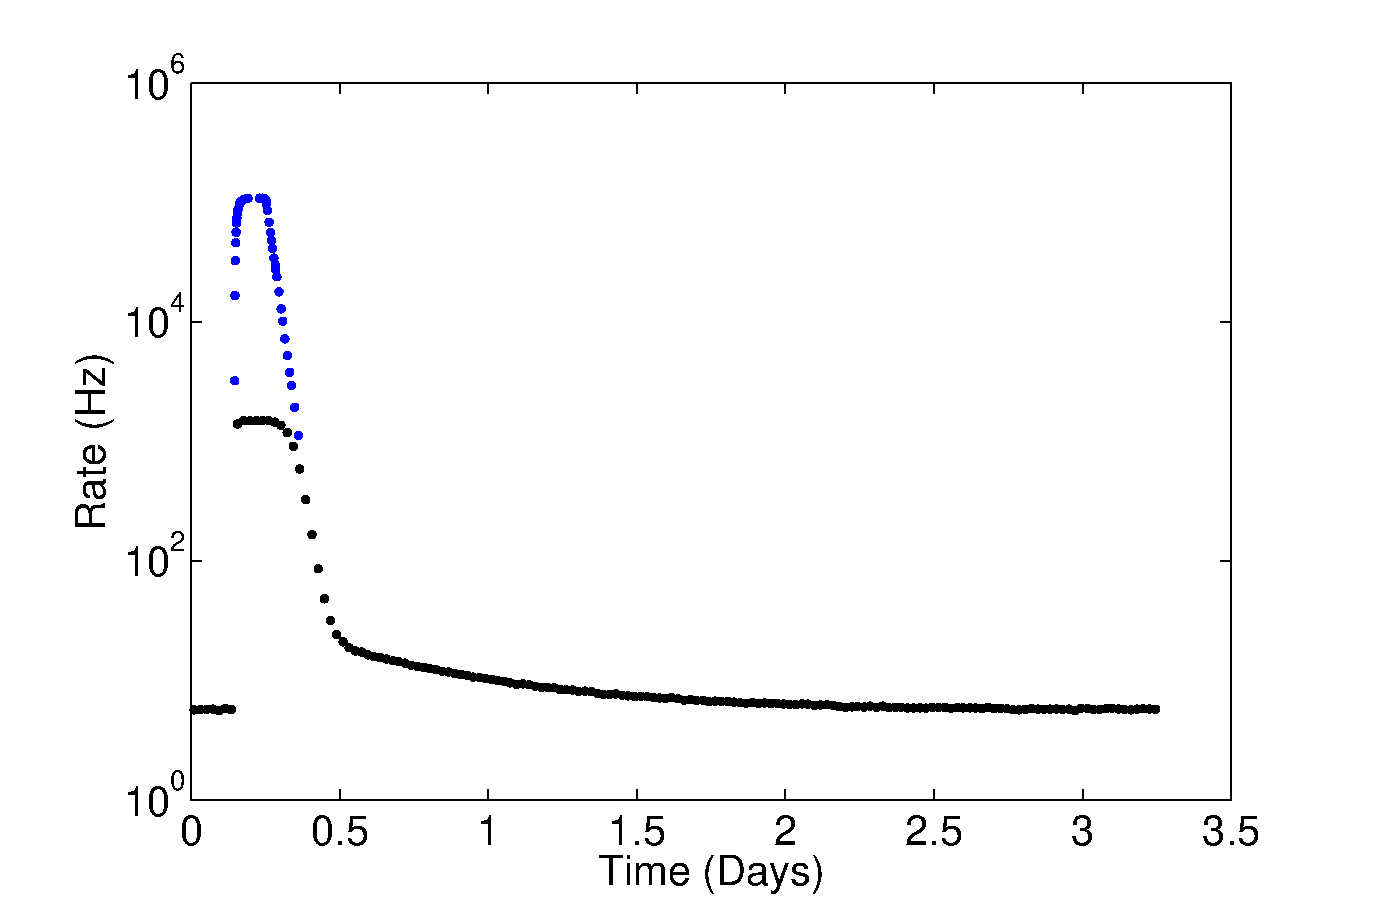
\includegraphics[width=80mm]{fig/TimeHisto_Analog2.eps}
\caption{The event rate versus time following a large CH$_3$T injection into a bench-top liquid xenon detector. Black points: the event rate measured with a dead-time limited digital DAQ system. Blue: true event rate measured with a fast analog scalar. In this experiment a maximum activity of 68,000 Hz was detected immediately after the injection, compared to a background count rate of 5 Hz. Initially the purifier is not included in the recirculation circuit, leading to a constant count rate. The count rate falls rapidly when the purifier is activated. At 0.5 days an elbow in the count rate is observed, indicating that outgassing of CH$_3$T from the detector plastics has become a limiting factor in the purification rate. }
\label{fig:Density}
\end{figure}


\section{Model of CH$_3$T removal}
\label{sec:appendix2}

We use a simple purification model to predict the CH$_3$T activity in LUX after an injection. The model is 

\begin{equation}
\frac{dC}{dt} = \frac{A}{V}J_{out} -\frac{C}{\tau},
\end{equation}

\noindent where  $C$ is the CH$_3$T concentration in the LXe,  $J_{out}$ is the flux of CH$_3$T out of the plastic components due to outgassing,  $A$ is the surface area of the plastic TPC cylinder, $V$ is the total volume of xenon in the active region, and $\tau$ is the characteristic removal time of CH$_3$T due to purification (5.9 hours). The model assumes perfect mixing of the fluid in the TPC. The initial concentration is the injection activity divided by the volume of the active region. We solve the model numerically with the Euler method while simultaneously solving the diffusion equation to determine $J_{out}$. The results predict the number of calibration events that may be collected and provide an estimate of when the CH$_3$T  decay rate will be small enough to allow the WIMP search to resume.

We approximate the diffusion into and out of the plastics as one-dimensional, since most plastics in LUX can be approximated as a thin cylindrical shell with no dependence on the azimuthal or $z$ coordinates.  Fick's laws in one dimension are

\begin{align}
J=-D\frac{d \phi(r,t)}{d r}  \\
\frac{d \phi}{d t} = D \frac{d^2 \phi(r,t)}{d r^2} 
\end{align}

\noindent 
where $J$ is the flux, $\phi(r,t)$ is the CH$_3$T  concentration in the plastic at depth $r$ and time $t$, and $D$ is the diffusion constant in the plastic. The concentration at the LXe-plastic boundary is fixed at $KC$, where K is the unitless solubility of CH$_3$T in the plastics. These equations are solved numerically and simultaneously with the purification model. 

$D$ and $K$ are not independently known for CH$_3$T in teflon or polyethylene at LXe temperature. However, only the combined quantity $G \equiv K \sqrt{ D/ \pi }$ is relevant as long as the diffusing substance does not reach the center of the plastic component (a good assumption for diffusion of CH$_3$T at LXe temperature). Under this condition, there exists an analytic solution to Fick's first law, which we evaluate at the LXe boundary:

%\begin{equation}
%\Scale[0.75]{\phi (x,t) = KC - \int \limits_0^t erf(\frac{x}{\sqrt{4D(t - \tau)}})K\frac{d}{d\tau}C(\tau)d\tau - KC(0)erf(\frac{x}{\sqrt{4Dt}}),}
%\end{equation}

\begin{equation}
J_{out}(t)= - G\left( \int \limits_0^t \frac{\frac{d}{dt'}C(t')}{\sqrt{t-t'}} dt' + \frac{C(0)}{\sqrt{t}}\right),
\end{equation}

\noindent
where the sign is reversed because the flux of material is outward. This result can be derived by applying Duhamel's principle along the infinite half-line, and it shows that the outgassing flux is linear in $G$. We set an upper limit of $G<0.0016 \frac{cm}{\sqrt{day}}$ for LUX based upon the data in Fig. \ref{fig:ch4_removal}. In that data the effect of $G$ would appear as an elbow in the CH$_4$ concentration versus time, as indicated by the blue line. The three data points near t = 3 days constrain the maximum value of $G$. We interpret this result as an upper limit because those data points are consistent with CH$_4$ backgrounds in the mass spectrometry system.

\begin{figure}[h!]
\centering
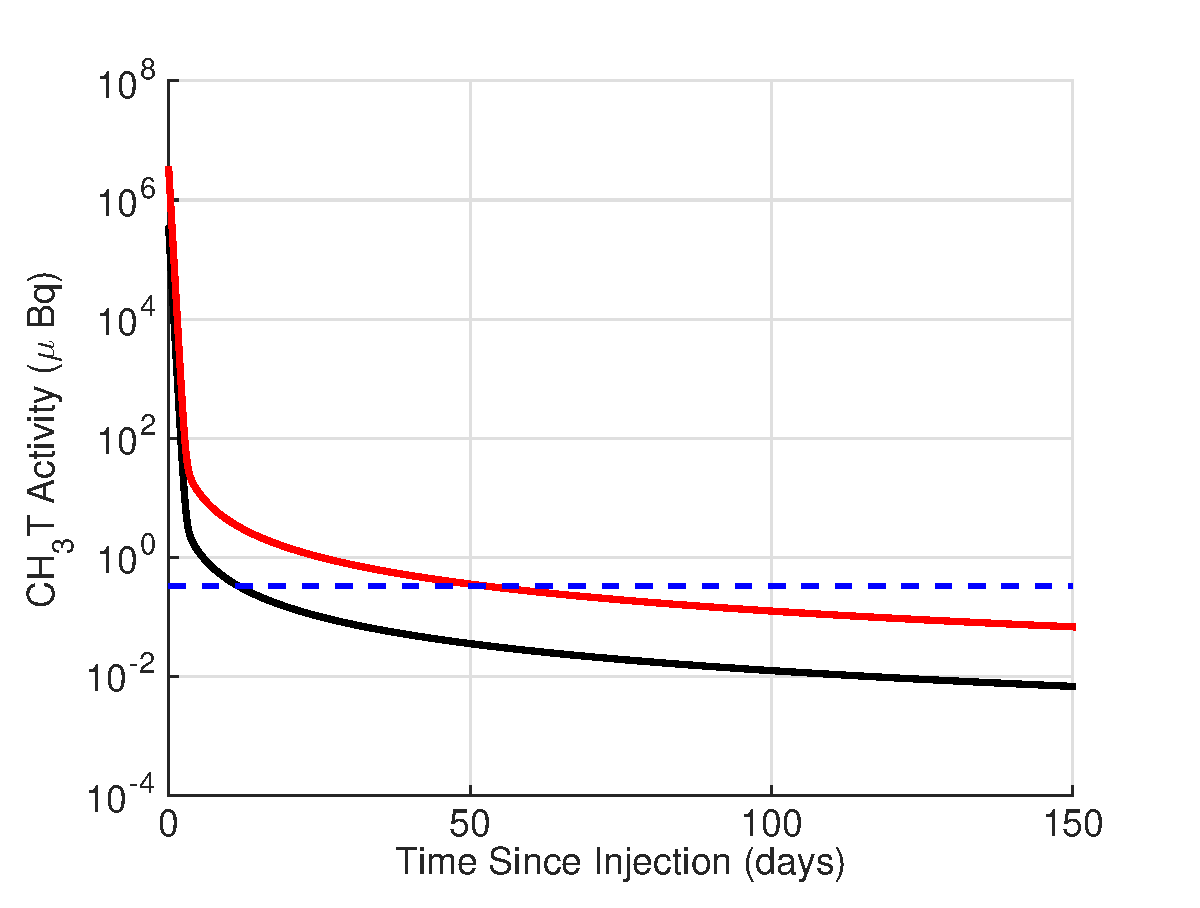
\includegraphics[width=0.95\textwidth]{fig/LUX_og_lim.eps}
\caption{Results of the purification model from 1 Bq (black curve) and 10 Bq (red curve) injections of CH$_3$T into LUX. The dashed blue line is the tritium activity goal of 0.33 $\mu$ Bq. The sharp initial fall is due to the 5.9 hour purification time constant of LUX, while the slow long-term removal is dominated by outgassing. The outgassing simulated here assumes  $G=0.0016$ cm/day$^{1/2}$).}
\label{fig:tau_var}
\end{figure}

Fig. \ref{fig:tau_var} shows the results of the purification model for a 1 Bq and 10 Bq injection into LUX assuming $G$ = 0.0016 cm/day$^{1/2}$  . We take 0.33 $\mu$Bq of residual CH$_3$T activity as an approximate goal for resuming WIMP search running, and we find that for injections on the order of 1 Bq we reach 0.33 $\mu$Bq eight days later, while 10 Bq injections may take as long as 35 days.  Ultimately the final decision regarding low background data quality is made during the data analysis phase, with guidance provided by the purification model described here.


\begin{acknowledgments}

This work was partially supported by the U.S. Department of Energy (DOE) under award numbers DE-FG02-08ER41549, DE-FG02-91ER40688, DE-FG02-95ER40917, DE-FG02-91ER40674, DE-NA0000979, DE-FG02-11ER41738, DE-SC0006605, DE-AC02-05CH11231, DE-AC52-07NA27344, and DE-FG01-91ER40618; the U.S. National Science Foundation under award numbers PHYS-0750671, PHY-0801536, PHY-1004661, PHY-1102470, PHY-1003660, PHY-1312561, PHY-1347449; the Research Corporation grant RA0350; the Center for Ultra-low Background Experiments in the Dakotas (CUBED); and the South Dakota School of Mines and Technology (SDSMT). LIP-Coimbra acknowledges funding from Funda\c{c}\~{a}o para a Ci\^{e}ncia e a Tecnologia (FCT) through the project-grant CERN/FP/123610/2011. Imperial College and Brown University thank the UK Royal Society for travel funds under the International Exchange Scheme (IE120804). The UK groups acknowledge institutional support from Imperial College London, University College London and Edinburgh University, and from the Science \& Technology Facilities Council for PhD studentship ST/K502042/1 (AB). The University of Edinburgh is a charitable body, registered in Scotland, with registration number SC005336. 

We gratefully acknowledge the logistical and technical support and the access to laboratory infrastructure provided to us by the Sanford Underground Research Facility (SURF) and its personnel at Lead, South Dakota. SURF was developed by the South Dakota Science and Technology Authority, with an important philanthropic donation from T. Denny Sanford, and is operated by Lawrence Berkeley National Laboratory for the Department of Energy, Office of High Energy Physics.

\end{acknowledgments}


%double blank page so that the table doesn't spill into the bibliography
\newpage
\thispagestyle{empty}
\mbox{}
\newpage
\thispagestyle{empty}
\mbox{}

\documentclass[12pt,twocolumn]{article}


\usepackage{amsmath}
\usepackage{graphicx}
\usepackage[capposition=bottom]{floatrow}
\usepackage{amssymb}
\usepackage{graphicx}
\usepackage{caption}
\usepackage{rotating}
\usepackage{afterpage}
\usepackage{float}
\usepackage{geometry}
\usepackage{titlesec}
\usepackage{epstopdf}

\usepackage{latexsym}
\usepackage{graphicx}
\usepackage{color}
\usepackage{array}
\usepackage{multirow}
\usepackage{wasysym}
\usepackage{verbatim}

\addtolength{\oddsidemargin}{-.875in}
\addtolength{\evensidemargin}{-.875in}
\addtolength{\textwidth}{1.75in}


\newcommand{\isot}[2]{$^{#2}$#1 }
\newcommand{\xeiso}{\isot{Xe}{136}}
\newcommand{\thsrc}{\isot{Th}{228}}
\newcommand{\cosrc}{\isot{Co}{60}}
\newcommand{\krsrc}{\isot{Kr}{83m}}
\newcommand{\cssrc}{\isot{Cs}{137}}
\newcommand{\nonubb}  {$0\nu \beta \beta$}

\renewcommand\thesection{\Roman{section}.}
\renewcommand\thesubsection{\Alph{subsection}.}
\titleformat{\section}[block]{\bfseries\filcenter}{\thesection}{1em}{}
\titleformat{\subsection}[block]{\bfseries\filcenter}{\thesubsection}{1em}{}

\begin{document}

\title{Internal calibration of the LUX detector using tritiated methane}
\author{LUX Collab List}

\twocolumn[
\begin{@twocolumnfalse}
\maketitle

 \begin{abstract}

We present measurements of the electron-recoil (ER) response of the LUX dark matter detector using an internal tritium calibration source. The large-statistics tritium dataset provides ideal single-beta events with high purity and good spatial uniformity. We report on the charge and light yields of liquid xenon at 180 V/cm and 105 V/cm with high accuracy down to 1.3~keV energies, investigate fluctuations in the ER band, measure the energy threshold of the detector, and validate the combined energy model. These results provide input to the LUX Run3 WIMP search \cite{lux-reanalysis}.

\end{abstract}



\end{@twocolumnfalse}
]


\section{Introduction}

The Large Underground Xenon experiment (LUX) is a WIMP search located at the 4850' level of the Sanford Underground Research Facility (SURF) in Lead, South Dakota~\cite{lux-nim}. LUX detects particle interactions in liquid xenon (LXe) via scintillation (S1) and ionization charge (S2) signals. The LXe is instrumented as a dual-phase time projection chamber (TPC), providing an energy measurement, position information in three dimensions, and single-scatter event identification. Electron-recoil (ER) and nuclear-recoil (NR) events are distinguished by the ratio of the charge and light signals (S2/S1). Results from the first LUX science run (Run 3) were first reported in Ref.~\cite{lux-prl}. An improved analysis of the Run 3 data is reported in Ref.~\cite{lux-reanalysis}.

The LUX is monitored and calibrated primarily with electron sources that can be dissolved in the LXe. Two such sources,  \krsrc~\cite{Kastens:2009rt, Baudis} and tritium ($^{3}$H), have been deployed in LUX, both providing a large sample of spatially uniform events. In this article we report results from the calibration of LUX with tritium, a single-beta emitter with a Q value of 18.6~keV electron-equivalent\footnote{ER events and NR events generally have different energy scales in LXe. In this article we interpret all events using the ER energy scale.}~\cite{Tritium_Q}. 

The tritium beta spectrum is well known both theoretically and experimentally. It has a broad peak at 2.5~keV and a mean energy of 5.6~keV~\cite{Tritium_Mean,Tritium_Eq,Drexlin:2013lha}. 64.2\% of the decays occur between 1 and 8~keV, the energy range of interest for WIMP searches. These characteristics make it an ideal source for studying the ER response of LUX.  $\rm ^{83m}$Kr, which is a source of 9.4~keV and 32.1~keV internal conversion electrons, is well suited for routine monitoring and for correcting the spatial and temporal variations of the S1 and S2 signals, but is less useful for studies of the S2/S1 ER discrimination variable because both conversion electrons are above the dark matter energy range, and because the S2 signals from the two electrons generally overlap in the detector due to the short half-life of the intermediate state (154~ns). External gamma sources, such as \cssrc,  are also used on occasion by LUX, but they are unable to produce a useful rate of fiducial single-scatter calibration events in LUX in the WIMP energy range of interest due to self-shielding. We note that the most important background in LUX is due to Compton scatters, and such events are expected to have similar properties to beta decays in the tritium energy range. Neutron sources and a neutron generator are also employed by LUX to study the response to NR events~\cite{DD-paper}.

We use tritiated methane (CH$_3$T) as the host molecule to deliver tritium activity into LUX. Compared to molecular tritium (T$_2$), CH$_3$T has several advantages. It does not adsorb onto surfaces like the T$_2$ molecule, and it does not interfere with charge transport in LXe. Also, because of its 12.3 year half-life, tritium must be removed from the detector by purification, and methane is amenable to chemical removal with standard noble gas purifiers~\cite{Dobi_CH4}. Note, however, that diffusion of tritium activity into plastic detector components during the calibration is an important concern, since that activity may later re-contaminate the LXe during the WIMP search runs.  In this respect, CH$_3$T is preferable over T$_2$ due to its larger molecular size and lower diffusion constant and solubility~\cite{miyake:1983}. We investigated the CH$_3$T contamination risk empirically with a series of bench-top tests prior to the first injection into LUX. These tests, which are described in Appendix \ref{sec:appendix1}, demonstrated that the injection and removal could be done without undue risk to the experiment. 

An initial tritium dataset of $\sim$7,000 fiducial events was obtained by LUX in August of 2013, and the results were reported in Ref~\cite{lux-prl}. Subsequently, in December 2013, we injected additional activity with a higher rate and obtained a fiducial tritium dataset of 170,000 events. This dataset is used to characterize the LUX ER band in Ref.~\cite{lux-reanalysis}. Except where otherwise noted, in this article we report results from the larger December 2013 dataset.

\section{Tritiated Methane Removal}
\label{sec:RD}

CH$_3$T removal efficiency of zirconium getters had previously been studied at the University of Maryland.  It was found that ..... [ATTILA'S PAPER]. Additionally, a table top gaseous xenon system was developed at the University of Maryland to examine the effects of residuals contamination after injecting CH$_3$T.  It was found that a SAES MC1-905F methane purifier placed in series immediately after the CH$_3$T source bottle was required to prevent tritium from non-methane species from contaminating the plumbing. Using the result of these two studies, a small scale tritiated methane injection system was integrated into a liquid xenon system at the University of Maryland.  After cumulatively injecting over 68,000 Bq of observed CH$_3$T we were able to achieve purification efficiencies ranging from 99.983\% - 100\%, with an average purification efficiency of 99.999\% in our liquid experiments, where we define our purification efficiency to be

\begin{center}
Purification Efficiency $= 1 - \frac{A - B}{I - B},$
\end{center}

\noindent
where $A$ is the background event rate after injecting CH$_3$T, $B$ is the background event rate prior to injecting CH$_3$T, and $I$ is the injected CH$_3$T activity as observed by out PMTs.  

\begin{figure}[h!]\centering
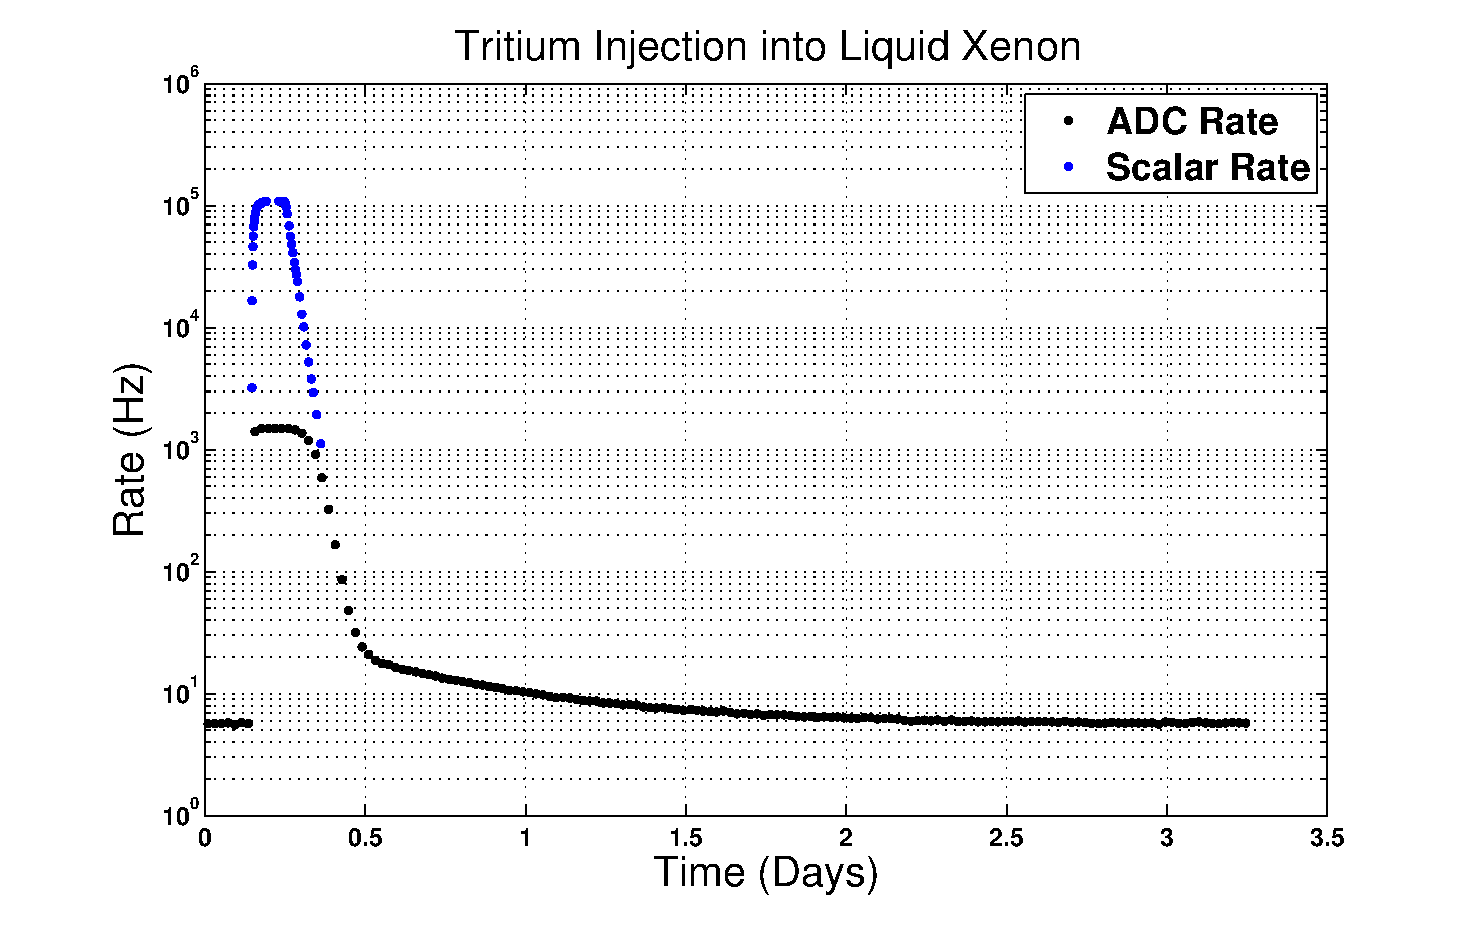
\includegraphics[width=100mm]{TimeHisto_Analog2.eps}
\caption{A time histogram of the event rate during a tritium injection into our small scale detector. The event rate greatly exceeded the limits of our ADC (black data points), so a analog scalar was used to count the true event rate (blue data points). }
\label{fig:Density}
\end{figure}


The liquid system was also used to study the effect of out gassing from plastics on the residual background rate after a CH$_3$T injection.  We found that the addition of plastic curtains around our PMTs does not impair our ability to remove CH$_3$T at $>$ 99.998\% levels. 

\section{Simulations}

\newcommand*{\Scale}[2][4]{\scalebox{#1}{$#2$}}%

Using Duhamel's priciple, the analytic solution to Fick's second law on a half-infite line is
\[\Scale[0.5]{\phi (x,t) = KC_{out} - \int \limits_0^t erf(\frac{x}{\sqrt{4D(t - \tau)}})K\dot{C_{out}}(\tau)d\tau - KC_{out}(0)erf(\frac{x}{\sqrt{4Dt}}),}\]
where $K$ is the solubility of the material, $D$ is the diffusion constant, and $C_{out}$ is the outside concentration of the material. \cite{Piche} For the out gassing process we are only able to detect the flux of material out of the plastic.  This is given by Fick's first law evaluated at $x=0$,
\[J_{out}(t)= - K \sqrt{\frac{D}{\pi}}( \int \limits_0^t \frac{\dot{C_{out}}(\tau)}{\sqrt{t-\tau}} d \tau + \frac{C_{out}(t)}{\sqrt{t}}),\]
where the sign has been flipped since the flux of material is outward.  We see that it is no longer possible to evaluate $K$ and $D$ separately, since the diffusion in and out of the plastic is completely determined by the time-dependent concentration outside of the plastic.  To simplify our model, we define a new constant
\[ G = K \sqrt{ \frac{D}{ \pi }} .\]

We can fit the integral of our equation for the flux out of the plastic over time to out gassing data collected in Maryland's liquid xenon system to extract a value for the constant $G$.  With this method we constrain $G \leq 0.01 \; \frac{cm}{\sqrt{day}}.$ 


\subsection{Implications for LUX}

With a constraint on $G$ taken from the analytic solution to Fick's second law, we turn to numerical simulation to answer the question of how much initial CH$_3$T activity to inject into LUX to meet our calibration conditions.  Several assumptions are made to simplify the numerical model.  First, we approximate the diffusion into plastic as being a one dimensional process.  Since the plastic in our detector at Maryland and in LUX can be approximated by a cylindrical shell, there is no dependence on the azimuthal or $z$ coordinates.  Since $r$ is large compared to the thickness of the plastic shell, $\frac{\delta^2 \phi}{\delta r^2} \gg \frac{1}{r} \frac {\delta \phi}{\delta r}$, so Fick's laws in a one dimensional approximation become
\[J=-D\frac{\delta \phi}{\delta r}\vec{r}\]
\[\frac{\delta \phi}{\delta t} = D \frac{\delta^2 \phi}{\delta r^2}.\]  We assume the concentration of CH$_3$T in LUX is uniform throughout its volume, since the design of LUX creates currents which stir the liquid xenon.  With perfect mixing the effect of the purifier can be modeled by adding an exponential time dependence to the outer volume.  The time constant of this decay has an upper limit equal to the time it takes xenon to recirculate through the LUX detector, although in reality the mass transport from diffusion in the liquid and gaseous xenon decreases this time constant. 

We use a simple implementation of the first order Euler method for our numerical simulations. The diffusion is simulated by setting the concentration at the boundary of the piece equal to $KC_{out}$, where $C_{out}$ is the concentration of CH$_3$T in the xenon.  This concentration is dependent on time according to
\[\frac{\delta C_{out}}{\delta t} = J_{out} \frac{A_{plastic}}{V_{xenon}}-\frac{C_{out}}{\tau},\]
where $A_{plastic}$ is the surface area of the plastic cylinder, $V_{xenon}$ is the total volume of xenon in the fiducial region, and $\tau$ is the time it takes for one full purification cycle.  The first term on the right of this equation models out gassing of CH$_3$T from the plastic cylinder, while the second term models removal of CH$_3$T through purification.  Using the first order Euler method, we arrive at an expression for $C_{out}$ given by
\[C_{j+1}=C_j + \Delta t [(J_{1,j}-J_{N_x,j})\frac{A_{plastic}}{V_{xenon}}-\frac{C_j}{\tau}].\]
The initial concentration is defined by dividing the desired injection activity by the volume of the fiducial region.  We choose $D = 2.3 \times 10^{-9} \frac {cm^2}{sec}$ so that the half-infinite boundary conditions in our diffusion model is valid, and combine this with our allowed range of values for $G$ to extract a value for $K$.  We use this model to predict the total number of calibration events as well as the time required to return to \textless 5\% of the nominal background rate for any CH$_3$T injection into LUX.  

\begin{figure}[h]
\centering
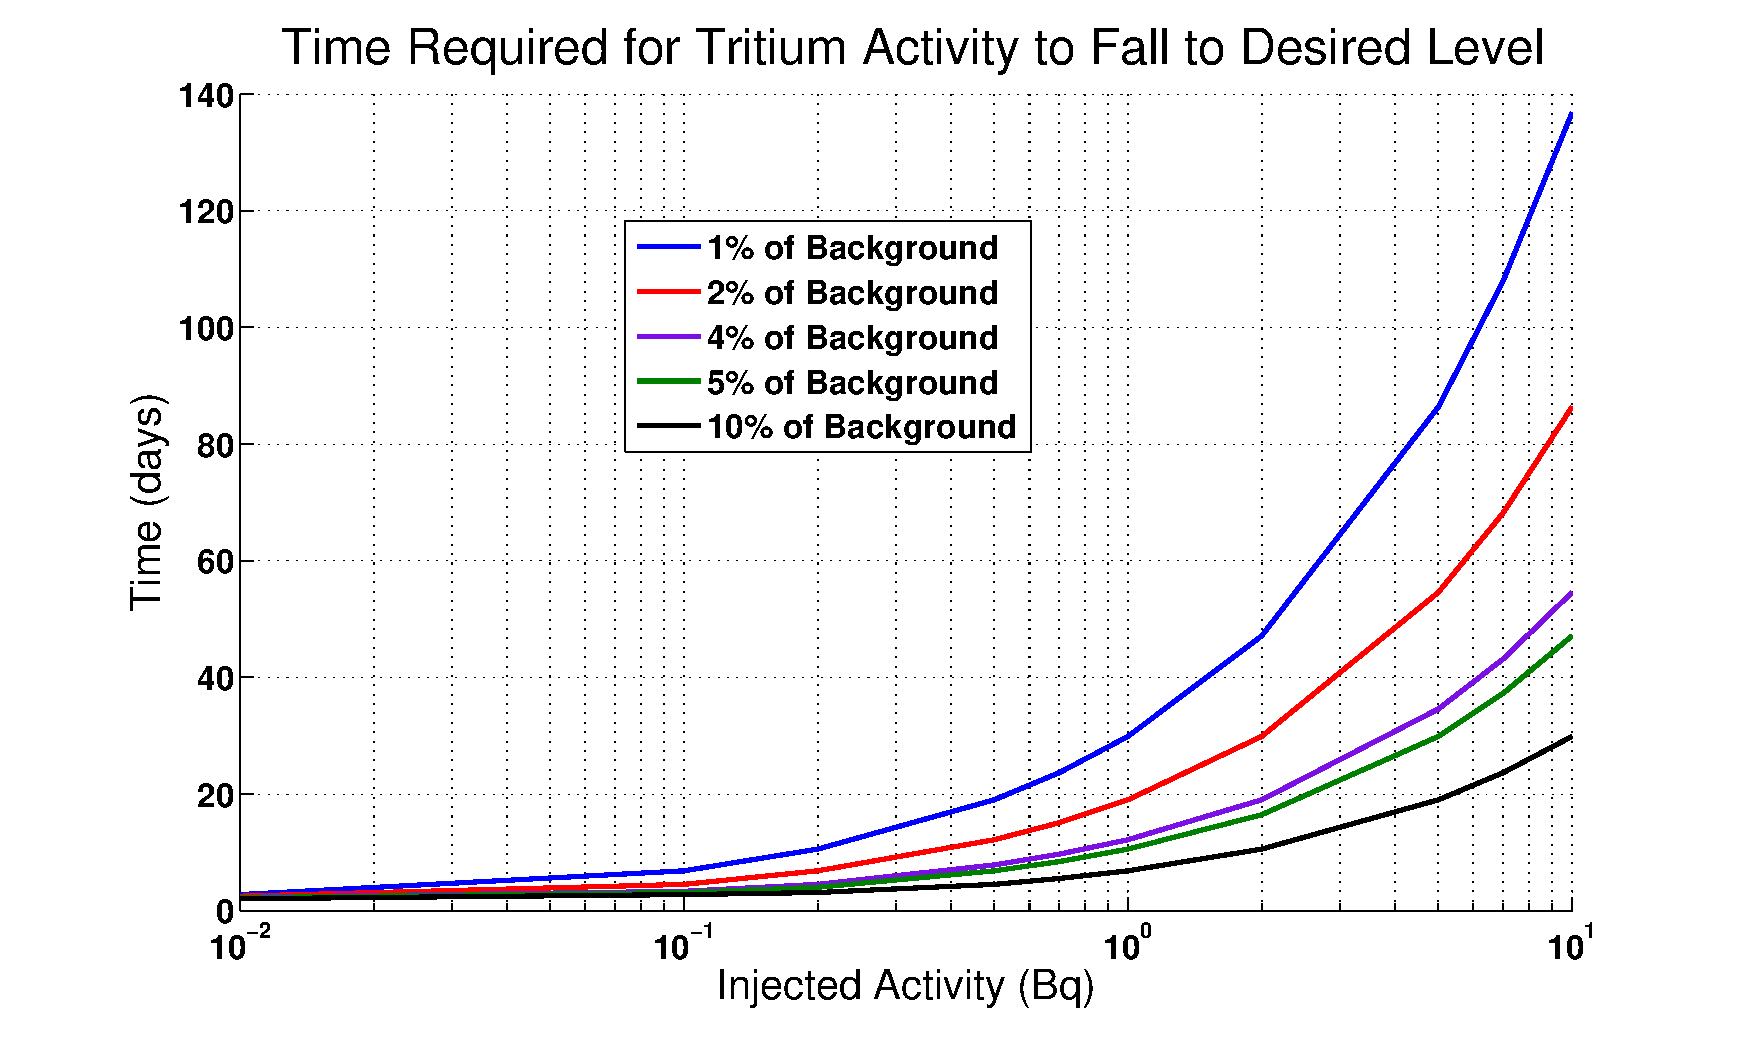
\includegraphics[scale=0.25]{LUXfig_INJvar_time_new.eps}
\caption{Time required to remove CH$_3$T from LUX after various injections.}
\label{fig:CH3TREMOVAL}
\end{figure}

\section{Experimental Setup}

The setup of our triated methane calibration technique can be separated into three parts: the injection system, the tritiated methane source bottle, and the zirconium getter.

\subsection{The tritiated methane source}

The tritiated methane source bottle for our calibration technique consists of a 2250 cc stainless steel bottle which is filled with a mixture of tritiated methane and xenon.  This source bottle was prepared in three steps.  First, we prepared a xenon bottle that had similar pressure and purity to the LUX system.  We filled a 2250 cc stainless steel bottle with 1590 torr of xenon from the same dekryptonation and purity program which the LUX xenon came from. The purpose of this xenon was to serve as a carrier gas for the triaited methane.  The next step was to prepare a small amount of tritiated methane to mix with this dekryptonated xenon.  A reservoir of tritiated methane with an activity of 204 Bq/torr-cc was purchased from Moravek Biochemical.  The reservoir was frozen with liquid nitrogen, resulting in a vapor pressure of 10.4 $\pm$ 0.05 torr.  We then opened the frozen tritiated methane reservoir to a 1/4" VCR cross which was sealed with swagelok valves on each side.  This first expansion space had a total volume of 5.2 $\pm$ 0.9 cc. Next, we isolated the VCR cross from the triated methane reservoir and then opened it to a 501 $\pm$ 0.2 cc expansion volume.  We isolated the VCR cross a second time and then opened it up to a 53.2 $\pm$ 3.4 cc expansion volume.  The VCR cross was then isolated for a third time before opening it to a 10.5 $\pm$ 0.5 cc expansion volume.  After this final expansion the VCR cross was isolated and the remaining 0.016 $\pm$ 0.006 torr-cc of tritiated methane left within was mixed with the dekryptonated xenon inside the 2250 cc bottle via cryopumping.  The final result was a tritiated methane source which had an activity of 9.1e-7 $\pm$ 3.4e-7 Bq/torr-cc.

\begin{figure}[H]
\centering
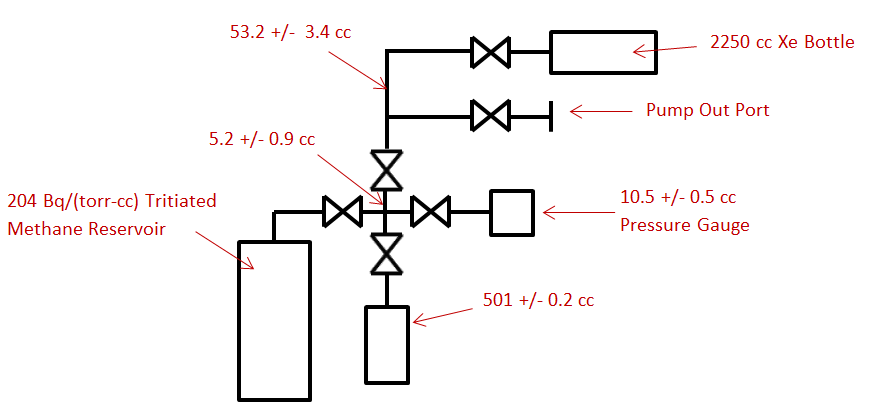
\includegraphics[scale=0.3]{BottleSetup.png}
\caption{The volume sharing system that was built to assemble our tritiated methane source bottle.}
\label{fig:BottleSetup}
\end{figure}


\subsection{The injection system}

The injection system for our tritiated methane calibration technique consists of a series of expansion volumes which are used to fine tune the amount of CH$_3$T that is injected.  Once the CH$_3$T source bottle is opened it flows through a methane gas purifier (SAES MC1-905F) to remove any sources of potential contamination, such as bare tritium.  The CH$_3$T then flows into the expansions volumes set by the user.  We use expansion volumes of 9.8 $\pm$ 0.4 cc , 13.3 $\pm$ 0.4 cc, 26.0 $\pm$ 0.5 cc, 82.7 $\pm$ 0.5 cc, 120.0 $/pm$ 0.6 cc, and 132.7 $\pm$ 0.6 cc in our experimental setup, giving us a range of 0.014 $\pm$  0.005 - 0.556 $\pm$ 0.208 Bq.  Once the expansion volumes have filled, the flow of xenon in the gas system is diverted through the expansion volumes to sweep the CH$_3$T into the detector.  We continue to flow through the expansion volumes for one hour, which is equivalent to flushing out the expansion volumes over 1000 times, since LUX flows at 20 SLPM and the full 384.5 cc of the expansion volumes are filled with 1590 torr of the xenon and CH$_3$T mixture.  A pump out port allows the expansion volumes to be evacuated in preparation for each use of the injection system.  Note that each injection will lower the total activity in the CH$_3$T source bottle via volume sharing, results in a smaller, yet calculable, injection activity with subsequent injections.  A pressure gauge (PT-T1) is included above the tritiated methane source bottle so that this drop in activity can be measured.  The final component of the injection system is a particle filter (Mott Corp. GSP3752FF11) which prevents particles contaminants from entering the detector.

\begin{figure}[H]
\centering
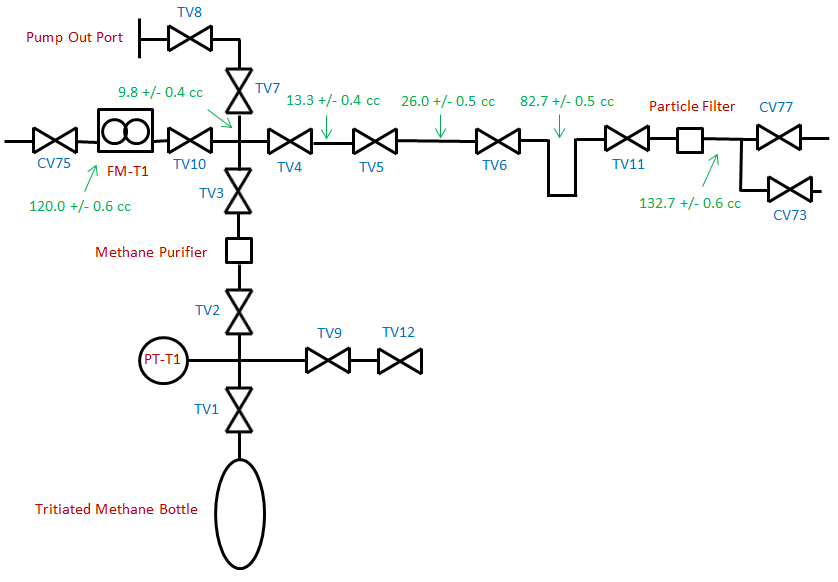
\includegraphics[scale=0.3]{TritiumPlumbingUpdated.png}
\caption{The injection system used in our CH$_3$T calibration technique. CV and TV labels indicate valves in the LUX circulation system and tritium injection system, respectively.  Expansion volumes are labeled in green, and other system components are labeled in red.}
\label{fig:LUXSys}
\end{figure}

\subsection{The zirconium getter}

The LUX gas system uses a hot zirconium getter (SAES-PS4MT15R1) downstream of the CH$_3$T injection system to remove CH$_3$T from the xenon.  Extensive R\&D was conducted using a smaller zirconium getter (SAES-PF4C3R1) at the University of Maryland to learn about the CH$_3$T removal efficiency of these purifiers.  Details of these studies is discussed in section \ref{sec:RD} 

\section{Injection Strategy}

The LUX collaboration agreed upon a three phase plan for a safe and successful tritium injection.  The first phase of this plan was a natural methane injection using the tritiated methane injection system for the purpose of determining the purification time constant in LUX.  The second phase of the plan was a small tritium injection (19 mBq) into LUX.  This small injection would highlight any potential problems before injecting a larger amount of tritium, and it would determine if any scaling factor was needed between the absolute injection activity and the observed injection activity.  Additionally, the small tritium injection would allow us to measure the fraction of tritium that goes into the fiducial volume.  Finally, the third phase of the plan was to use what we learned from the first two phases to safely inject a larger amount of tritium (15,000 events) for the purpose of measuring the ER rejection factor of LUX and cross-checking the NEST prediction of the ER band.

\subsection{Phase One}

During phase one 0.02 grams of natural methane were injected into LUX using the tritium injection system.  Purity samples from the detector were collected over the next few days, and a purification time constant of 5.90 $\pm$ 0.07 hours was determined using data collected with the LUX gas sampling system.

\begin{figure}[H]
\centering
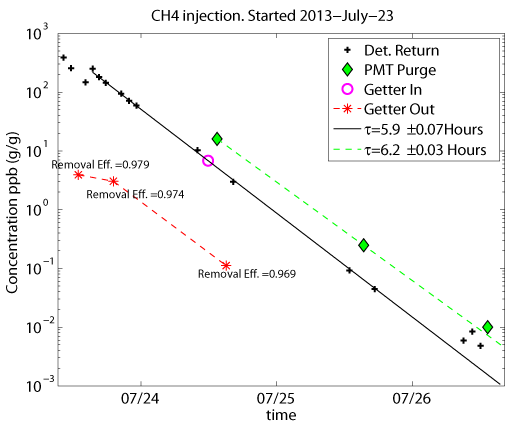
\includegraphics[scale=0.3]{CH4_injection.png}
\caption{First three days of the natural methane injection.  The discontinuity near the beginning of the data is due to a secondary natural methane injection.}
\label{fig:CH4Inject}
\end{figure}

\subsection{Phase Two and Three}

The first, smaller tritiated methane injection on Aug-08-2013 was done to confirm the purification model established by a natural methane purification campaign the previous week. An absolute activity of 20 mBq of tritiated methane was injected, while actively purifying. A purification time constant of 6.7 hours was observed, consistent with the natural methane purification rate measured by the sampling system. After a day of circulating through the getter the tritium decay had fallen below detectable amounts confirming the effective removal of the tritiated methane with the getter. On Aug-13-2013 a larger injection of 800 mBq was performed. The second injection produced 20,000 beta decay events in the LUX detector before being completely removed, 5000 of those events could be used the calibrate the ER band in the WIMP search region of 0-30 Phe (pulse area in photo electrons). 
Figure \ref{fig:Removal} shows the two tritium injections and the subsequent CH3T purification. Figure \ref{fig:Removal_2} shows the rate of events in the ER band before and after the tritium injection and removal. The CH3T was injected at the getter output but had passed through a special methane purifier to remove O2 and H2O or other impurities that could cause a degradation in election lifetime. The injections were performed with the getter in purify mode to maintain detector purity, as soon as the CH3T was injected is was immediately being removed.  The rate of tritiated methane removal was consistent with the removal of natural methane observed by the xenon sampling system which was used to first verify the removal of methane to $\rm 1/10^5$. Figure \ref{fig:Removal}.


\begin{figure}[H]\centering
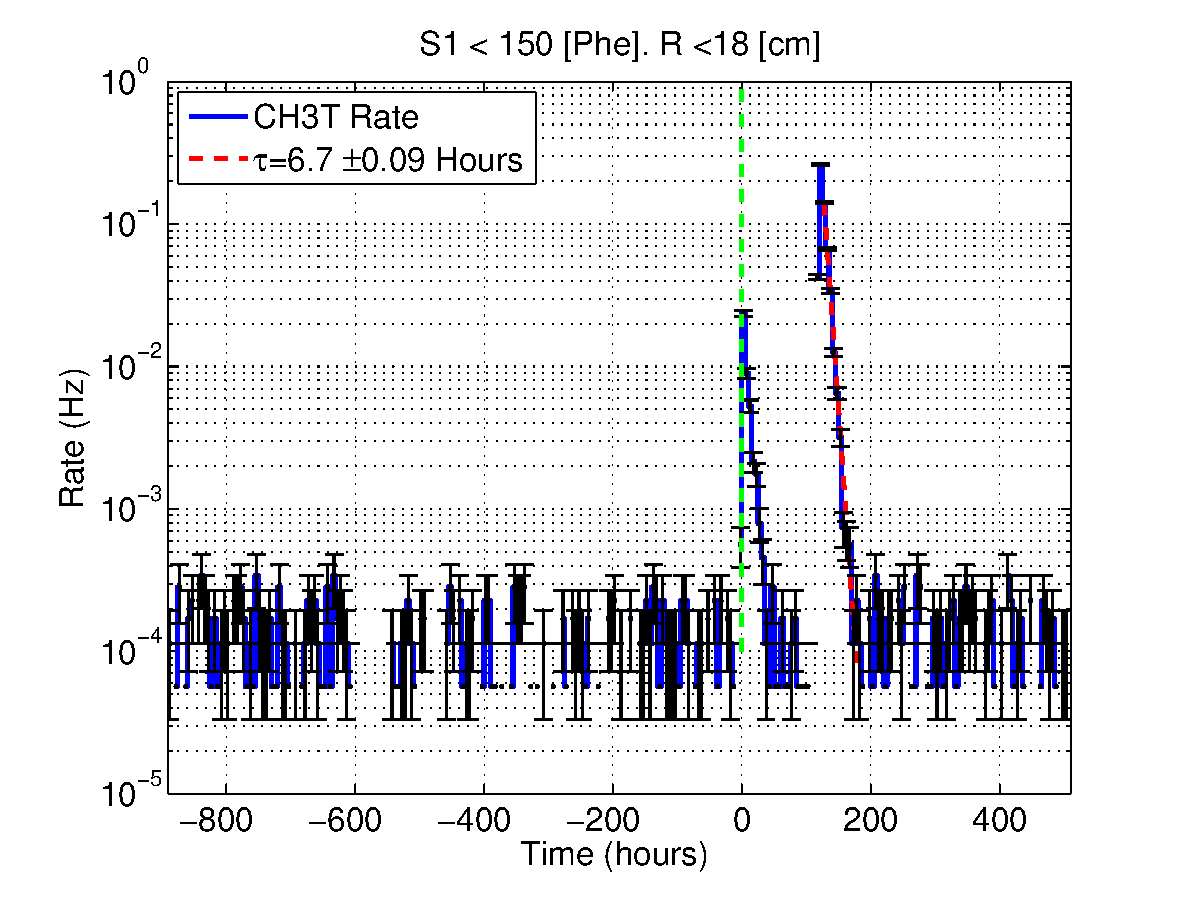
\includegraphics[width=80mm]{CH3T_Rate_fid_150_lux10_20130813T1120_note.eps}
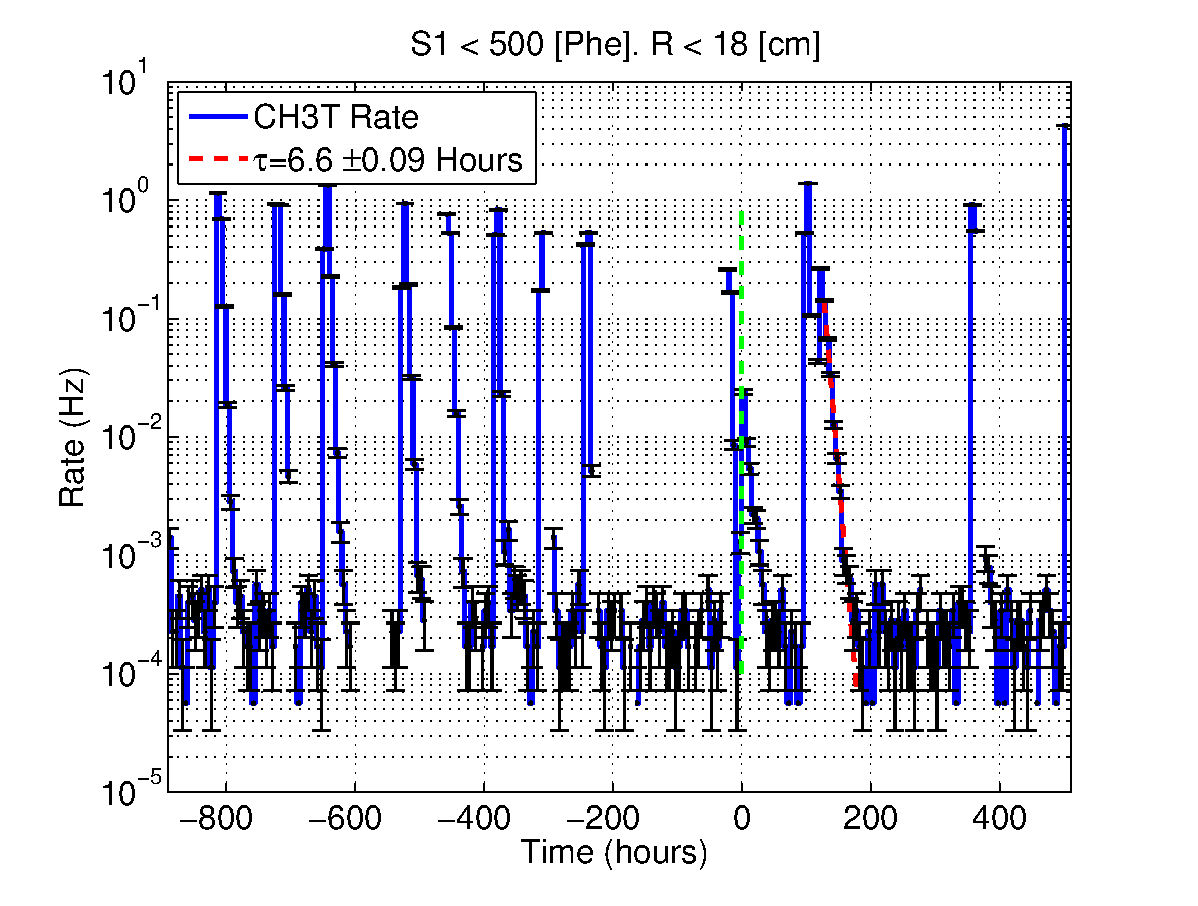
\includegraphics[width=80mm]{CH3T_Rate_fid_500_lux10_20130813T1120.eps}
\caption{Left: Rate of events in the WIMP search region over a two month window. The dashed, vertical green line represents the time of the fist tritiated methane injection. Right: The S1 threshold extended to 500 Phe to include rate spikes from the $\rm ^{83}Kr$ injections, used for detector calibration during the science run. }
\label{fig:Removal}
\end{figure}

\begin{figure}[H]\centering
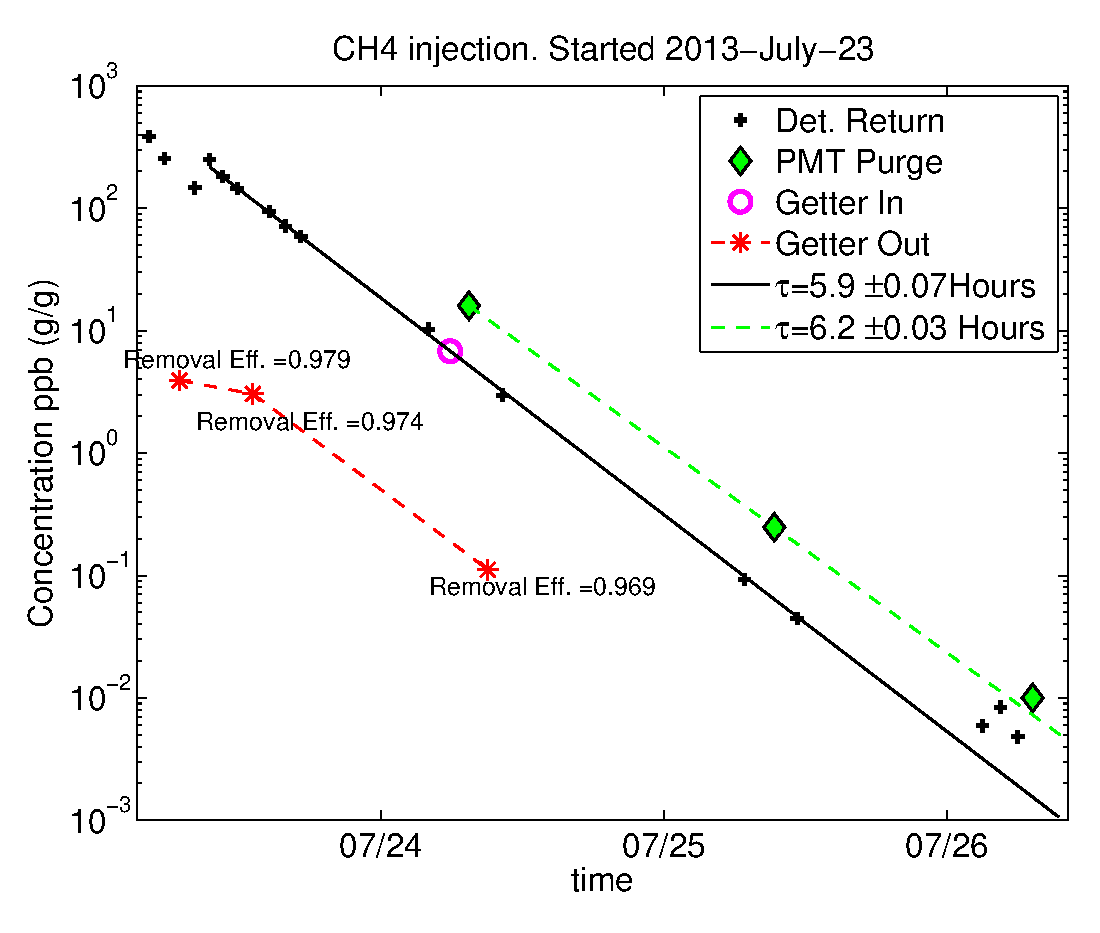
\includegraphics[width=80mm]{CH4_injection.eps}
\caption{Removal of natural methane observed by the xenon sampling system prior to the tritiated methane injections. }
\label{fig:Removal}
\end{figure}


\begin{figure}[H]\centering
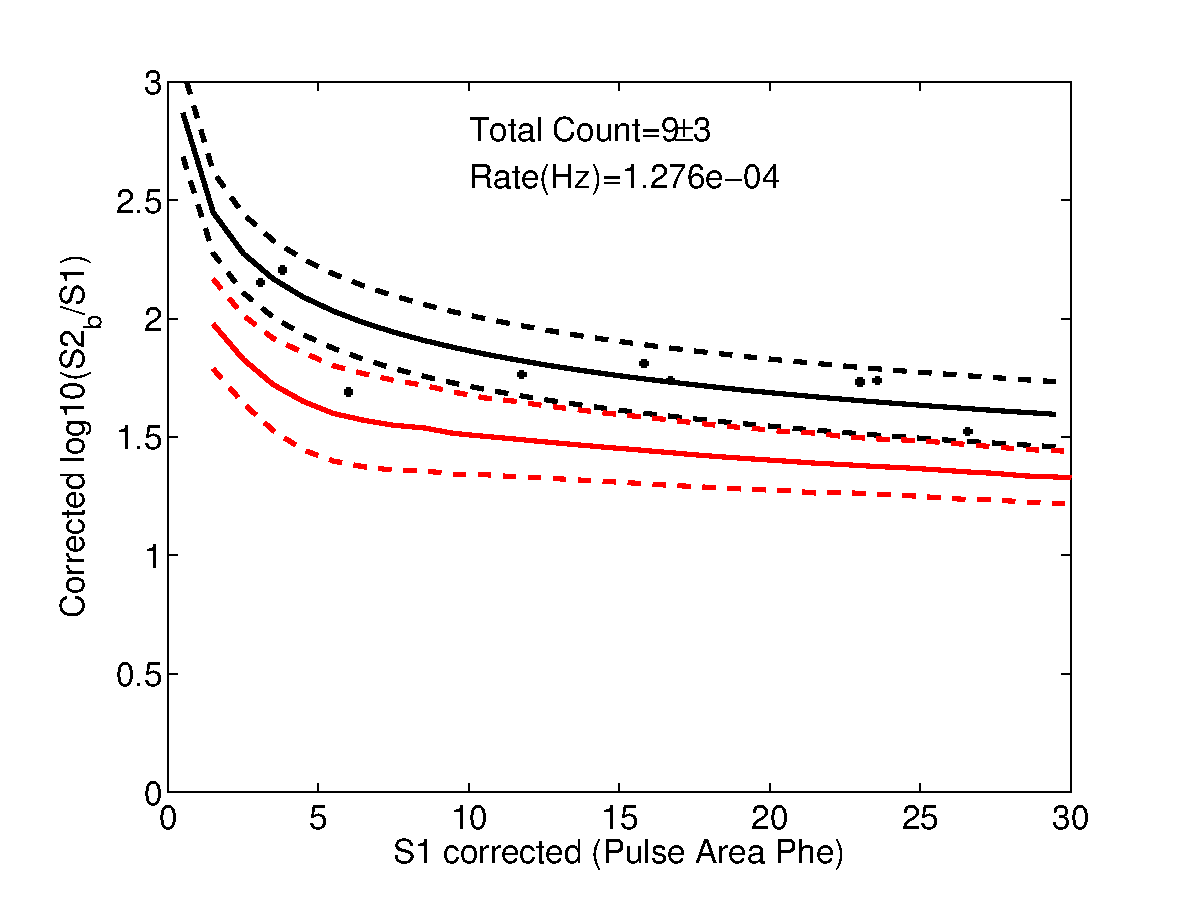
\includegraphics[width=80mm]{CH3T_fid_30_before_100_18_lux10_20130813T1120_cp05328_note.eps}
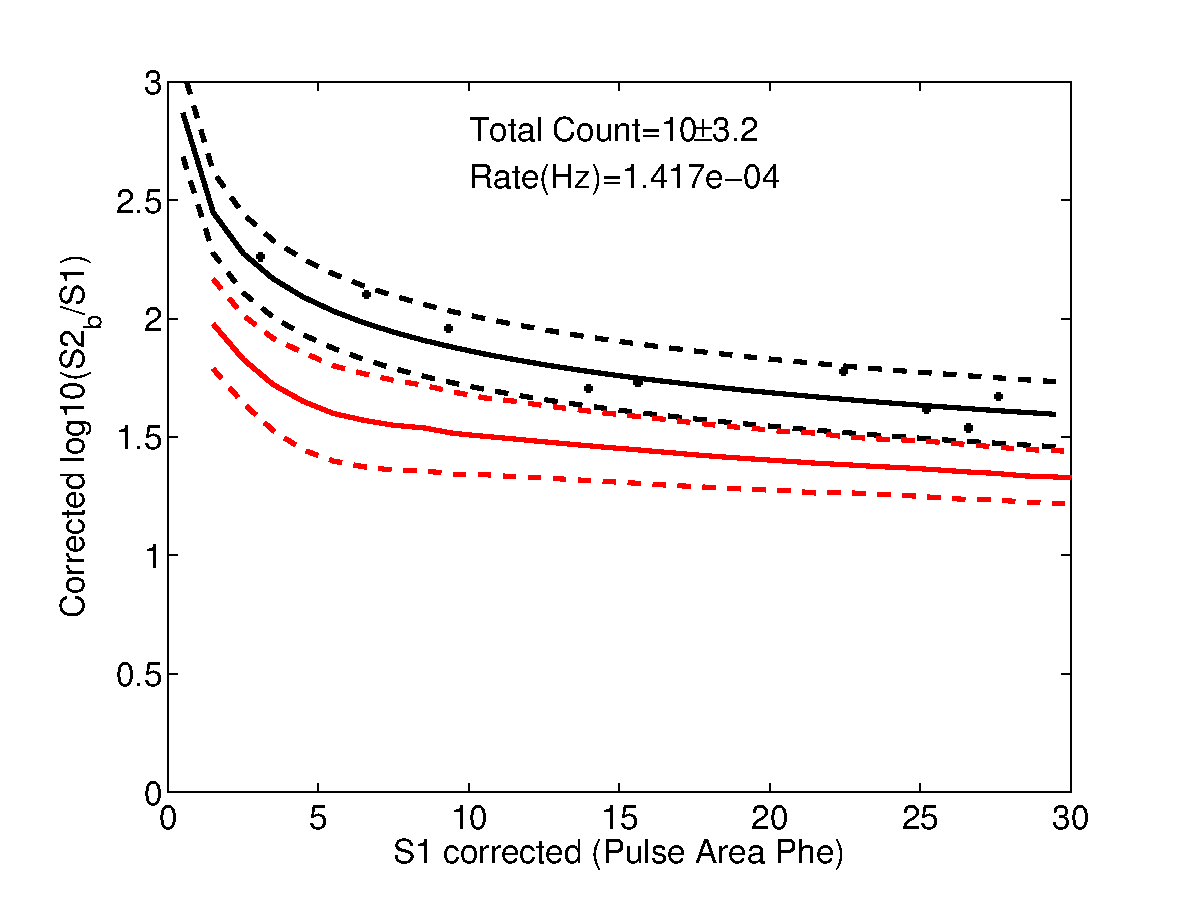
\includegraphics[width=80mm]{CH3T_fid_30_after_100_18_afterlux10_20130813T1120_cp05328_note.eps}
\caption{Left: 100 Hour time window in the WIMP search region before the tritiated methane injection. Right: 100 Hour time window in the WIMP search region after the purification of the tritiated methane. }
\label{fig:Removal_2}
\end{figure}

   


\section{Results from the Tritiated Methane Calibration}



\subsection{Mixing of Tritiated Methane in Liquid Xenon}

Tritium events appear uniformly distributed in the liquid volume several minutes after injecting the tritiated methane inline with the xenon gas circulation path. Figure \ref{fig:Density} shows the XY and Z distribution of tritium events thirty minutes after an injection. The events shown cover the region from the gate to the cathode and radially out to the edge of the detector. An additional cut requiring that the event be between $\rm \pm 3 \sigma$ of the ER mean was made to diregard residual alpha events from the walls and cathode, the event rate consisted overwhelmingly of tritium events. The tritiated methane dispersed uniformly throughout the liquid xenon illuminating all regions on the detector. 
 
\begin{figure}[h!]\centering
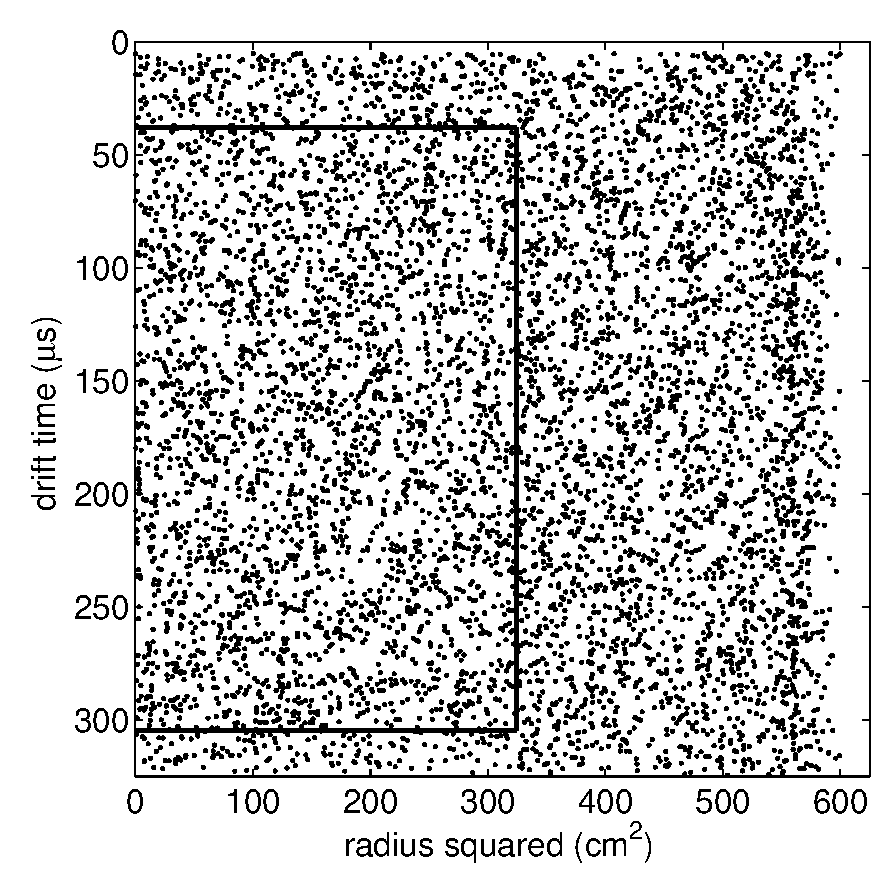
\includegraphics[width=80mm]{CH3T_RZ_scatter_lux10_20130812T1546.eps}
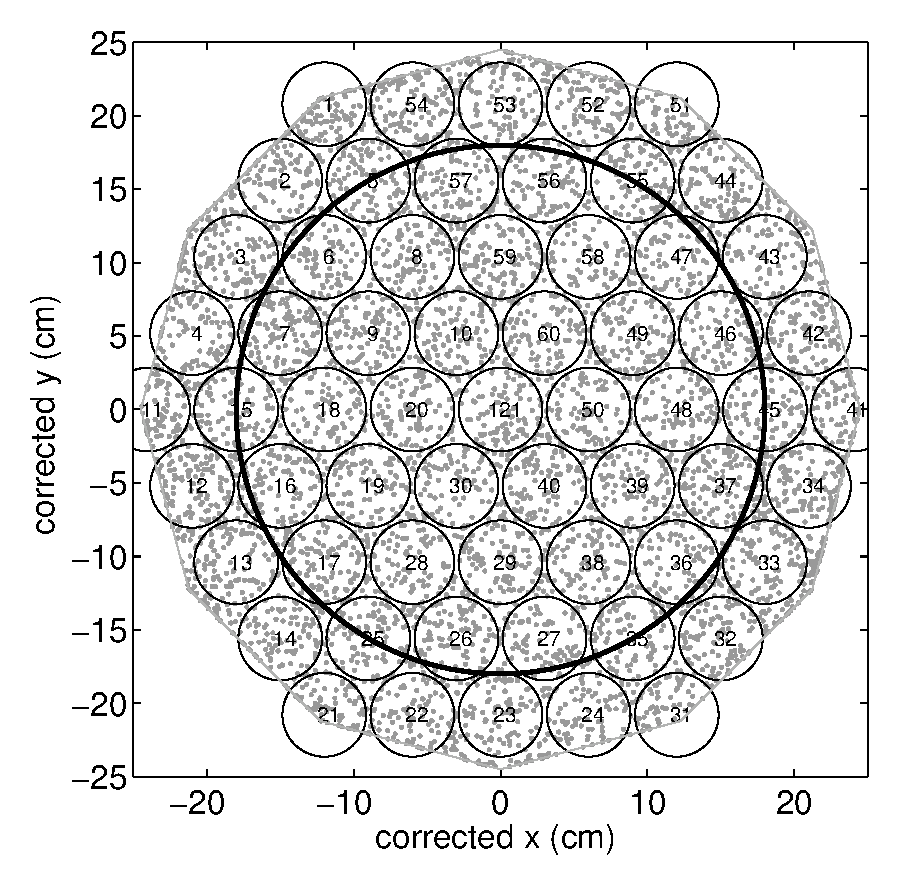
\includegraphics[width=80mm]{CH3T_XY_scatter_PMT_lux10_20130812T1546.eps}
%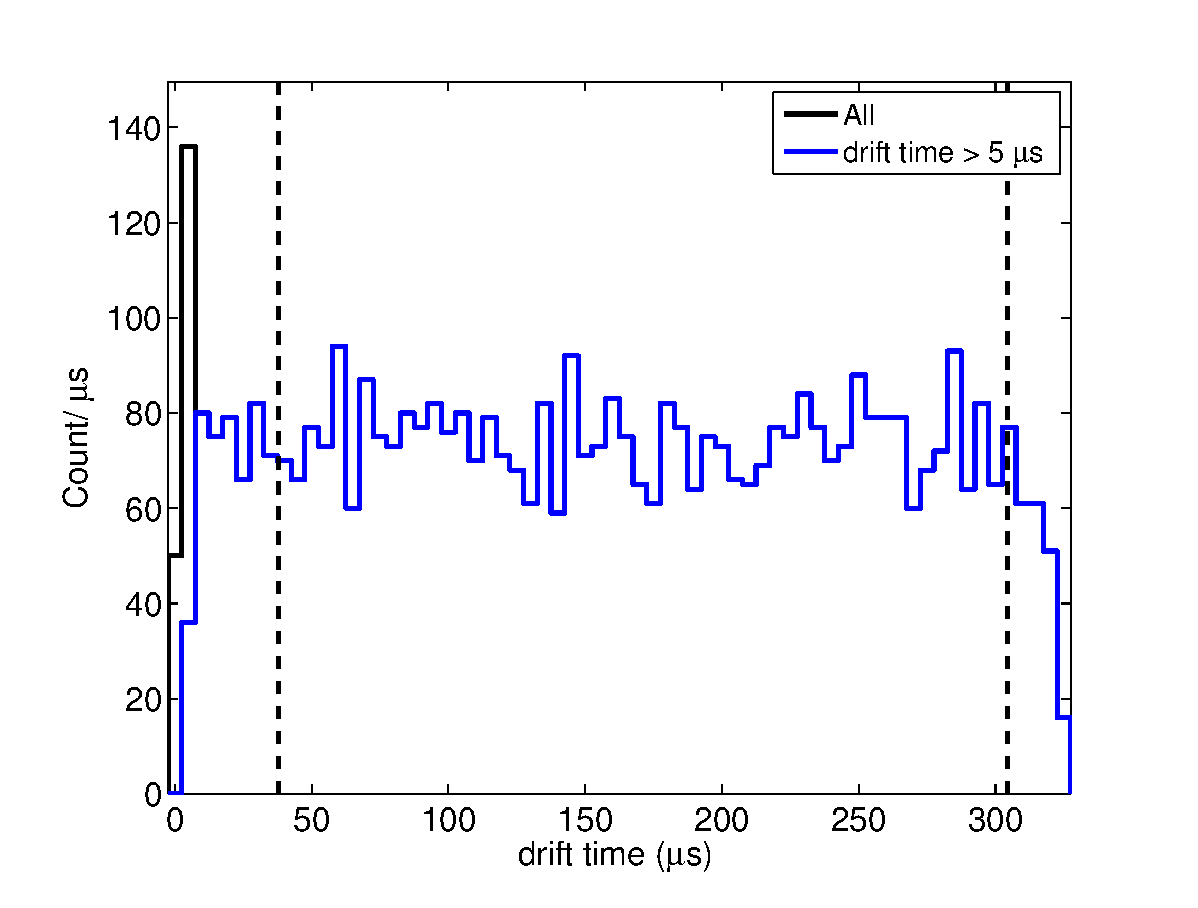
\includegraphics[width=80mm]{CH3T_Z_density_lux10_20130812T1546.eps} %> No Need R^2 vs. Z figure contains Z information
\caption{Left: The distribution of tritium events vs. detector radius squared. The solid black line represents the fiducial volume. Right: The distribution of tritium events vs. XY in the region between the gate and the cathode. The solid black line represents the fiducial volume and the black circles represent the locations of PMTs (photo multiplier tubes).}
\label{fig:Density}
\end{figure}




  \begin{comment}
... Remove this graphic, for smaller tritium injection
\begin{figure}[h!]\centering
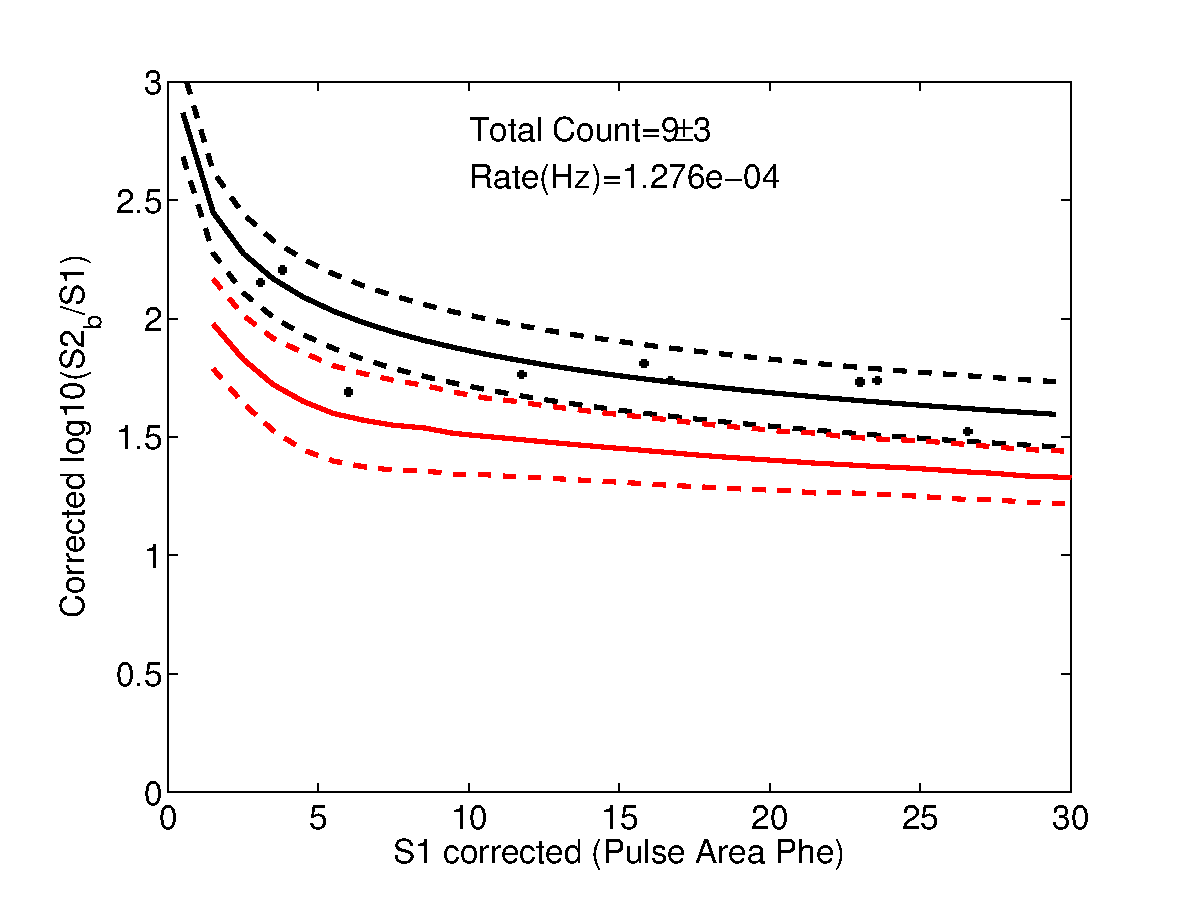
\includegraphics[width=80mm]{CH3T_fid_30_before_100_18_lux10_20130813T1120_cp05328_note.eps}
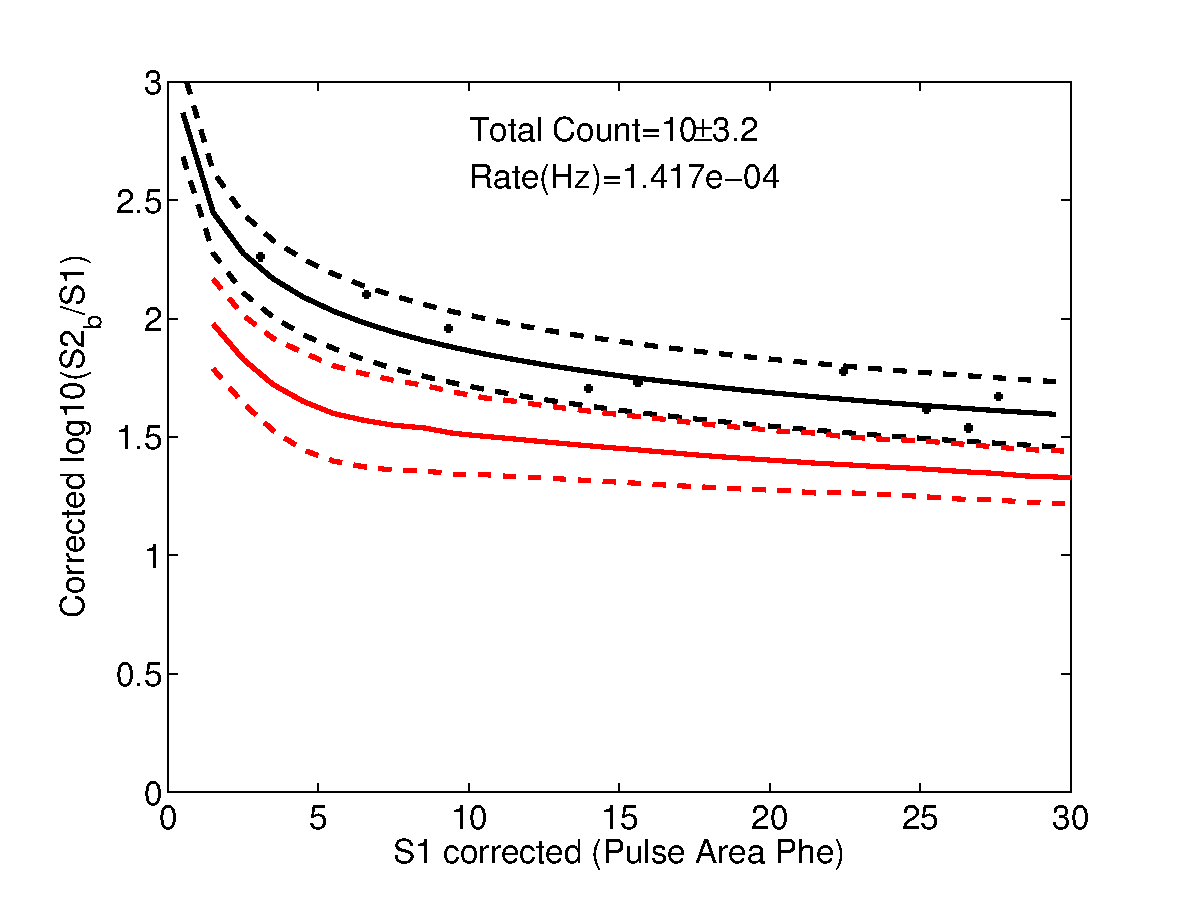
\includegraphics[width=80mm]{CH3T_fid_30_after_100_18_afterlux10_20130813T1120_cp05328_note.eps}
\caption{Left: 100 Hour time window in the WIMP search region before the tritiated methane injection. Right: 100 Hour time window in the WIMP search region after the purification of the tritiated methane. }
\label{fig:Removal_2}
\end{figure}

  \end{comment}

\subsection{Definition of Electronic Recoil Band and Comparison with NEST Model}

Using the tritium source we calibrated the electronic recoil band in the fiducial volume of the LUX detector to unprecedented accuracy. Figure \ref{fig:Band} shows the mean of the ER band along with the 10-90\% confidence bounds ($\pm 1.28\sigma$) obtained from the beta decay of tritium at a drift field of 180 V/cm. The results of the leakage fraction at 50\% NR acceptance per each 1 Phe bins in S1 are shown in \ref{fig:Leak}. The nuclear recoil band, in red, is defined by the NEST model along with AmBe and $\rm^{252}Cf$  calibrations. Methane will not quench xenon scintillation [\cite{Kirill_Methane}] shows that if methane is introduced into the xenon at a relative concentration of a few percent, then the amount of scintillation produced by the mixture is reduced by a factor of two compared to pure xenon. But for our application we require a methane concentration of only one part in $\rm10^{15}$, and therefore our methane injection will not have any negative effects on scintillation production and transport.

WIMPs primarily interact with the atomic nuclei xenon atoms in LUX resulting in nuclear recoils whereas the vast majority of residual radioactivity within the detector are gammas which result in electronic recoils. Thus, knowing the separation of the ER from the NR band allows for a measure of the background rejection of a liquid xenon WIMP search experiment. We define the measure of background rejection as leakage fraction, reported here as the fraction of events in the ER band that spill into the lower half of the NR band. Over 115,000 tritium decays were used for the ER band calibration, between 1-50 Phe in S1 (1-8 $\rm keV_{ee}$), and were found using standard WIMP search cuts within the fiducial volume. A figure of merit for ER and NR discrimination is the leakage fraction defined as  the number of tritium events populating the lower half of the NR band are compared to the total number of tritium events in the selected energy range. 
%$\rm (1-erf((Mean\_ER-Mean\_NR)/(sqrt(2)*sigma\_ER)))/2 $.
Figure \ref{fig:Leak} shows the leakage fraction per 1 Phe bins in S1. The mean leakage fraction in the region used for the LUX 2013 PRL results, between 1-30 Phe (1-5 $\rm keV_{ee}$) in the fiducial, was found to be 0.42\% $\rm \pm$ 0.02\%, see Figure \ref{fig:Leak}. In the 40 hour time window in which the data was acquired less than three out of 115,000 events are expected to be non tritium [BG paper reference]. The NR band used is from NEST version 0.98 and is vetted with AmBe, $\rm^{252}Cf$ and DD neutron generator calibrations.


\begin{figure}[h!]\centering
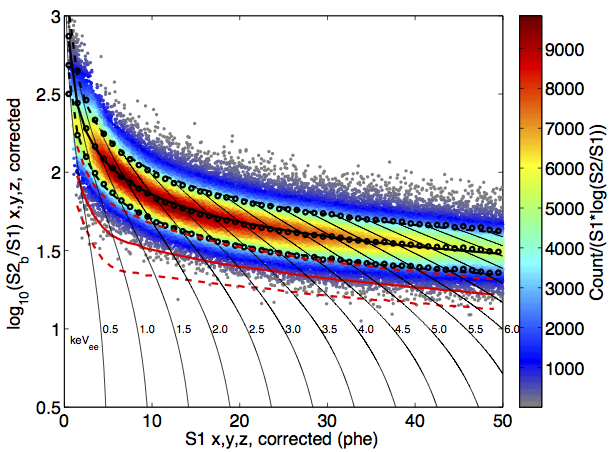
\includegraphics[width=80mm]{CH3T_fid_50_2_Dec_Tritium_Approval_Plots.png}
\caption{Discrimination vs. S1 using over 115,000 tritium beta decays between 1 and 50 Phe in S1 (about $\rm1-8 keV_{ee}$). On average from 1 to 30 Phe the discrimination is 99.58\%, defined by the fraction of events of events below the mean of the nuclear recoil band. The red band represents the NEST nuclear recoil band (version 0.98) vetted with an AmBe, $\rm^{252}Cf$ and DD neutron generator calibration.}
\label{fig:Band}
\end{figure}

\begin{figure}[h!]\centering
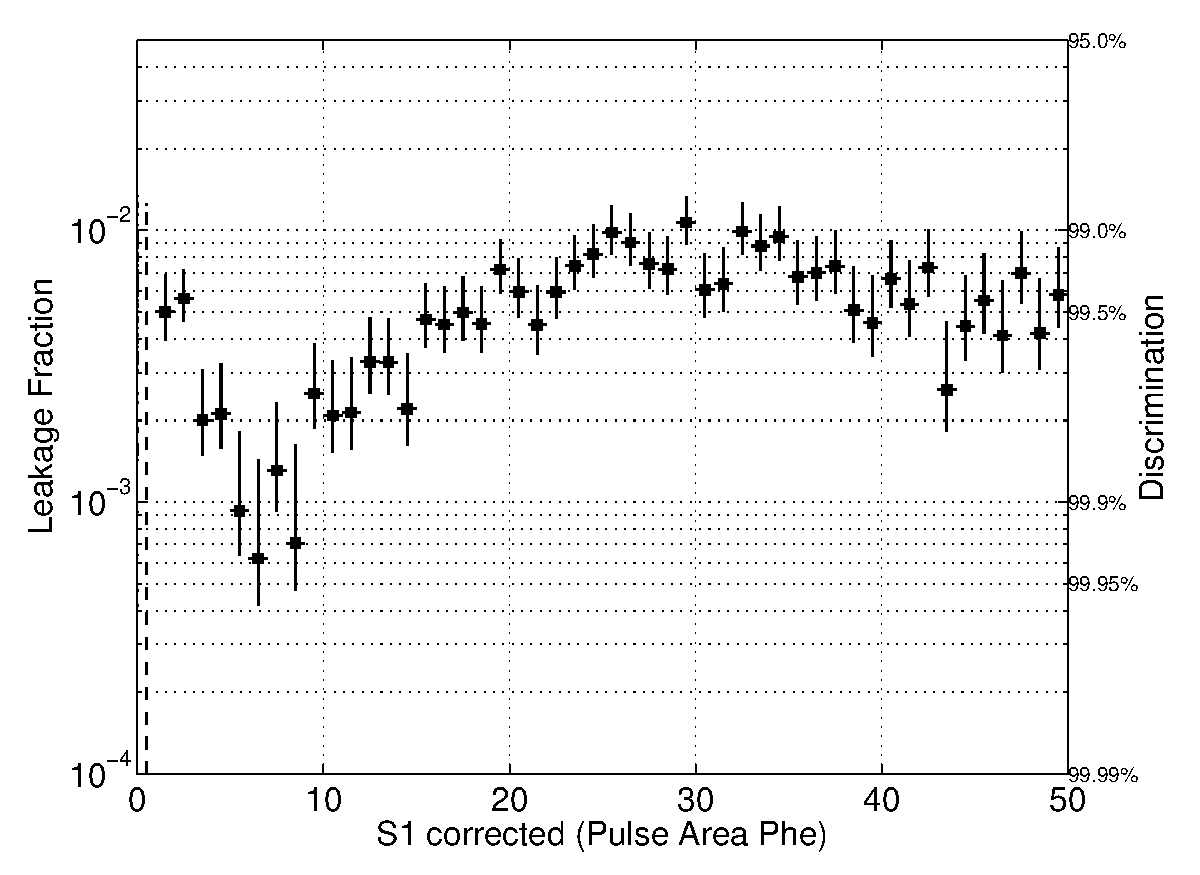
\includegraphics[width=80mm]{CH3T_Leakage_fid_50_Dec_Tritium_Approval_Plots.eps}
\caption{Discrimination vs. S1 using over 115,000 tritium beta decays between 1 and 50 Phe in S1 (about $\rm1-8 keV_{ee}$). On average from 1 to 30 Phe the discrimination is 99.58\%, defined by the fraction of events of events below the mean of the nuclear recoil band. The red band represents the NEST nuclear recoil band (version 4c) vetted with an AmBe, $\rm^{252}Cf$ and DD neutron generator calibration.}
\label{fig:Leak}
\end{figure}


%Figure \ref{fig:NEST_v_Data} shows the comparison between simulation(NEST) and the data for the ER band. The agreement between simulation and data is good down to 7 Phe in S1. This is expected since at sub 2 $\rm keV{ee}$ (7 Phe in S1) data is limited and the NEST model has yet to be vetted at such low energies[Matthew/ Erik Dahl Thesis]. The newly acquired ER data below 2 $\rm keV{ee}$ from tritium will be used improve upon the NEST model at the extration field of 180 V/cm [ref?].

\begin{comment}

\begin{figure}[h!]\centering
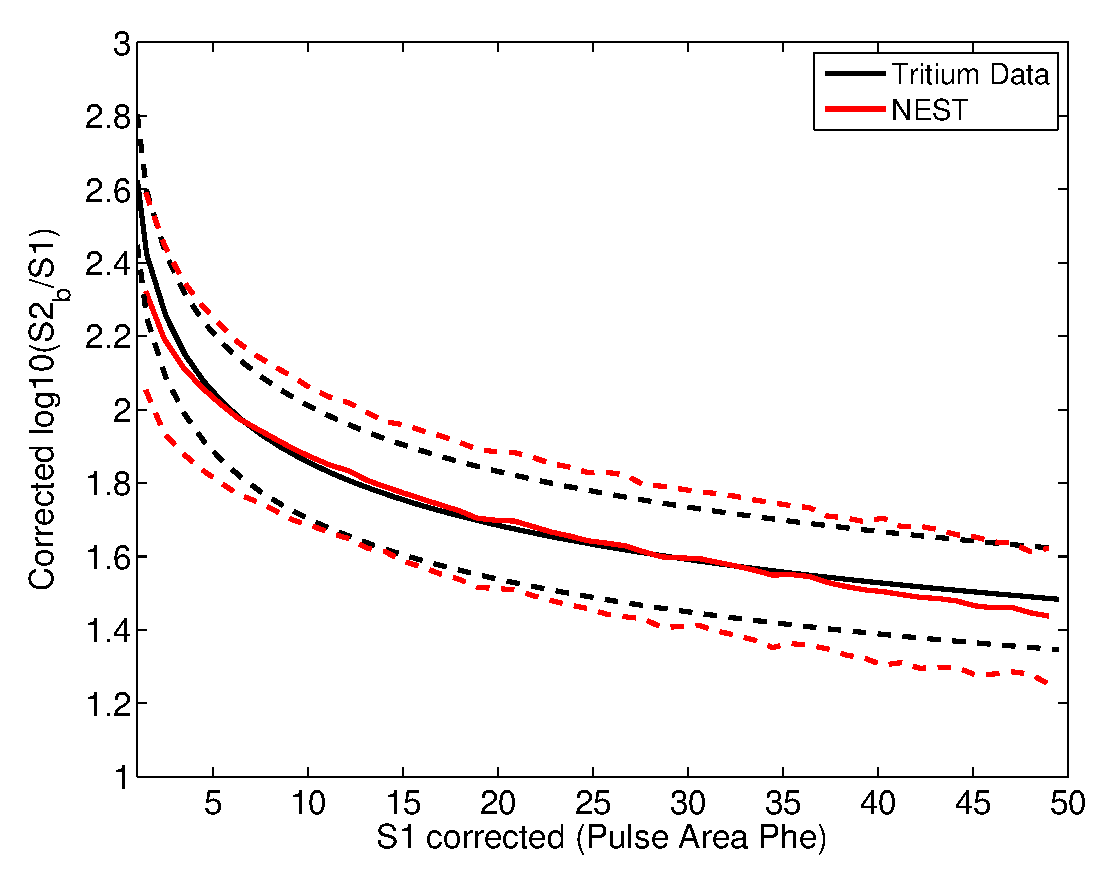
\includegraphics[width=80mm]{CH3T_DATA_NEST_fid_30_LUX_SIM_Tritium.eps}
\caption{ER band measured using tritium data in black with 90\% confidence bounds ( $\rm \pm 1.3 \sigma$) compared with the NEST prediction in red.}
\label{fig:NEST_v_Data}
\end{figure}
\end{comment}

%%%%%%%%%%%%%%%%%%%%%%%%%%%%%%%%%%%%%%%%%%%%%%%%%
\begin{comment}

\subsection{Threshold Determination}

The tritiated methane calibration source can also be used to determine detector efficiency for both S1 (primary scintillation) and S2 (secondary scintillation) down to sub 1 keV electronic recoils.The ultimate limitation of single scatter event is typically the S1 since the signal size of the S1 is one to three orders of magnitude less than the S2. We measured the threshold by comparing the NEST model of a tritium beta spectrum to the data, we find good agreement to the threshold determined from LED calibration, figure \ref{fig:S1S2_Thresh}(need to add to plot). The threshold for the S2 (bottom PMT array) shown is entirely due to the S1 threshold. We use only the bottom PMT array for the S2 signal because the secondary scintillation light is more uniformly distributed along the bottom PMTs than the top PMTs. Figure \ref{fig:E_spec} shows the tritium beta spectrum measured in the LUX detector along with the NEST prediction, note at the 180 V/cm drift field NEST has been vetted form 2 to 10 $\rm keV{ee}$.

\begin{figure}[h!]\centering
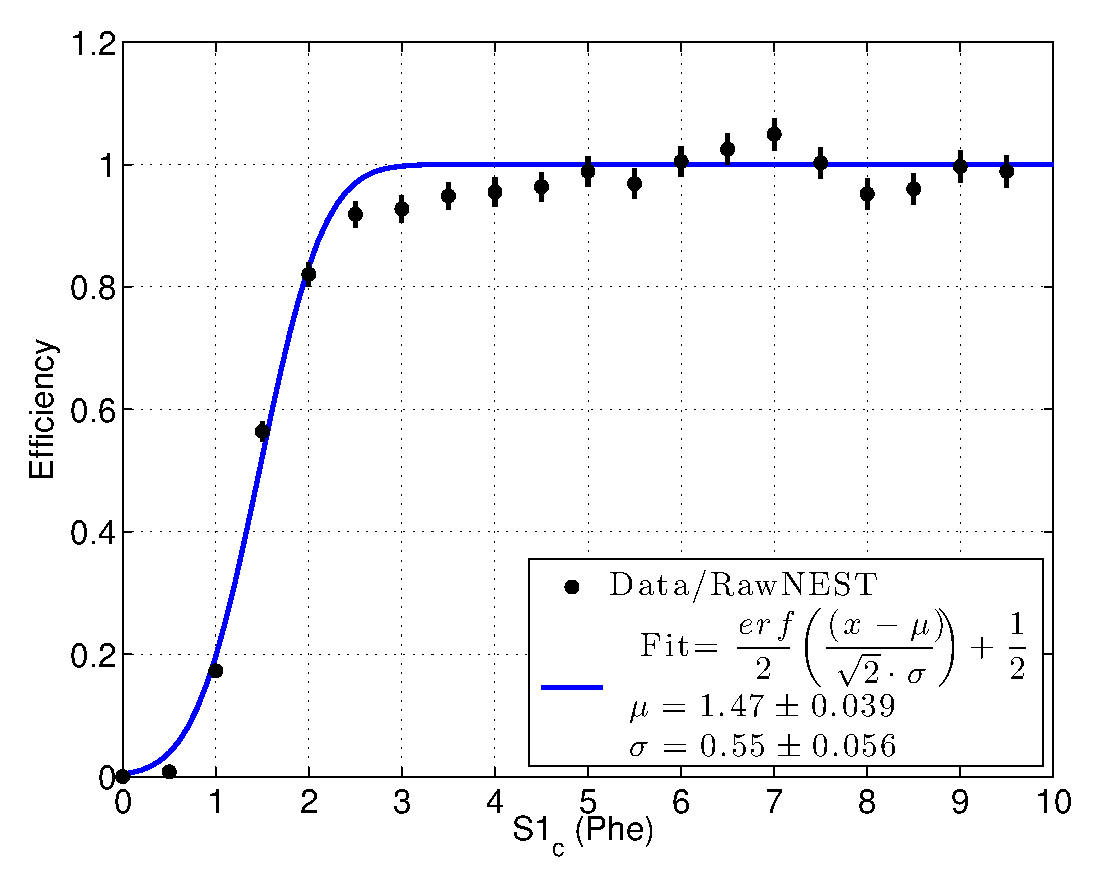
\includegraphics[width=80mm]{CH3T_eff_S1_100_T_paper_corr_threshold.eps}
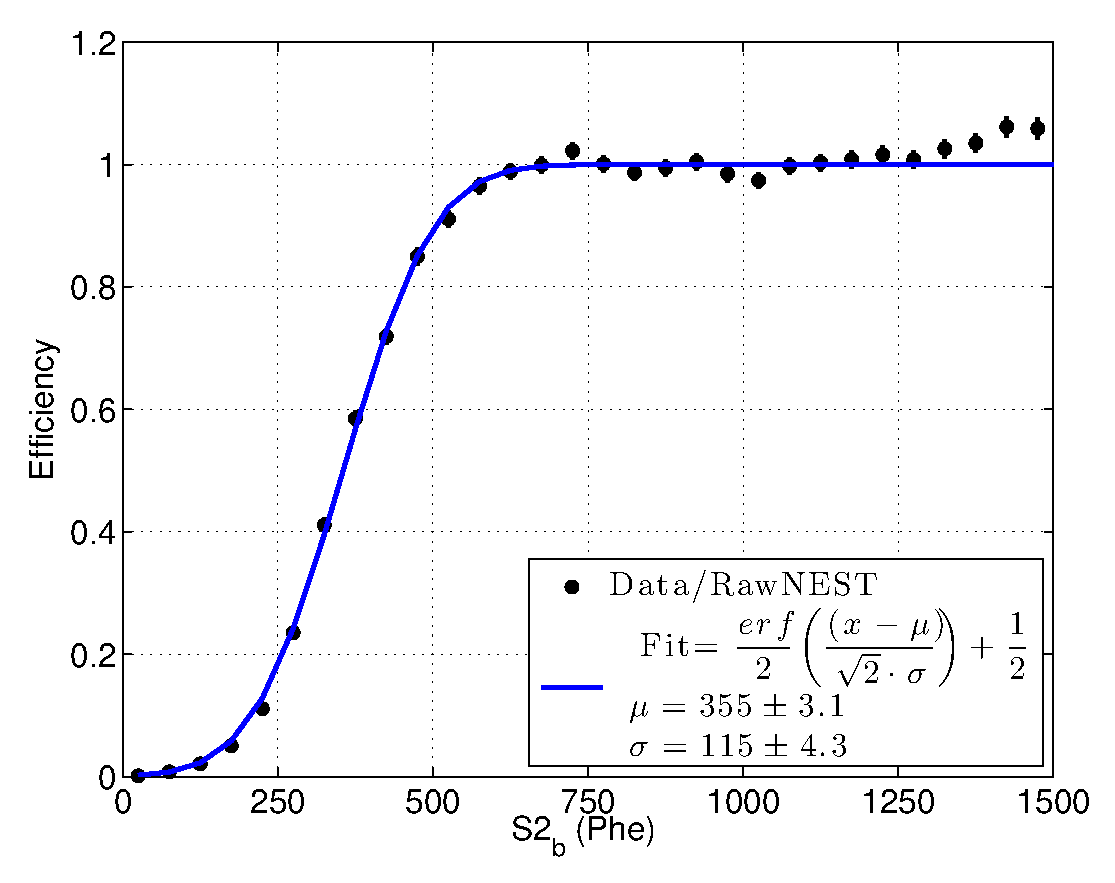
\includegraphics[width=80mm]{CH3T_eff_S2_100_T_paper_corr_threshold.eps}
\caption{S1 Threshold determined from Tritium. S2 Threshold determined from Tritium.}
\label{fig:S1S2_Thresh}
\end{figure}



\begin{figure}[h!]\centering
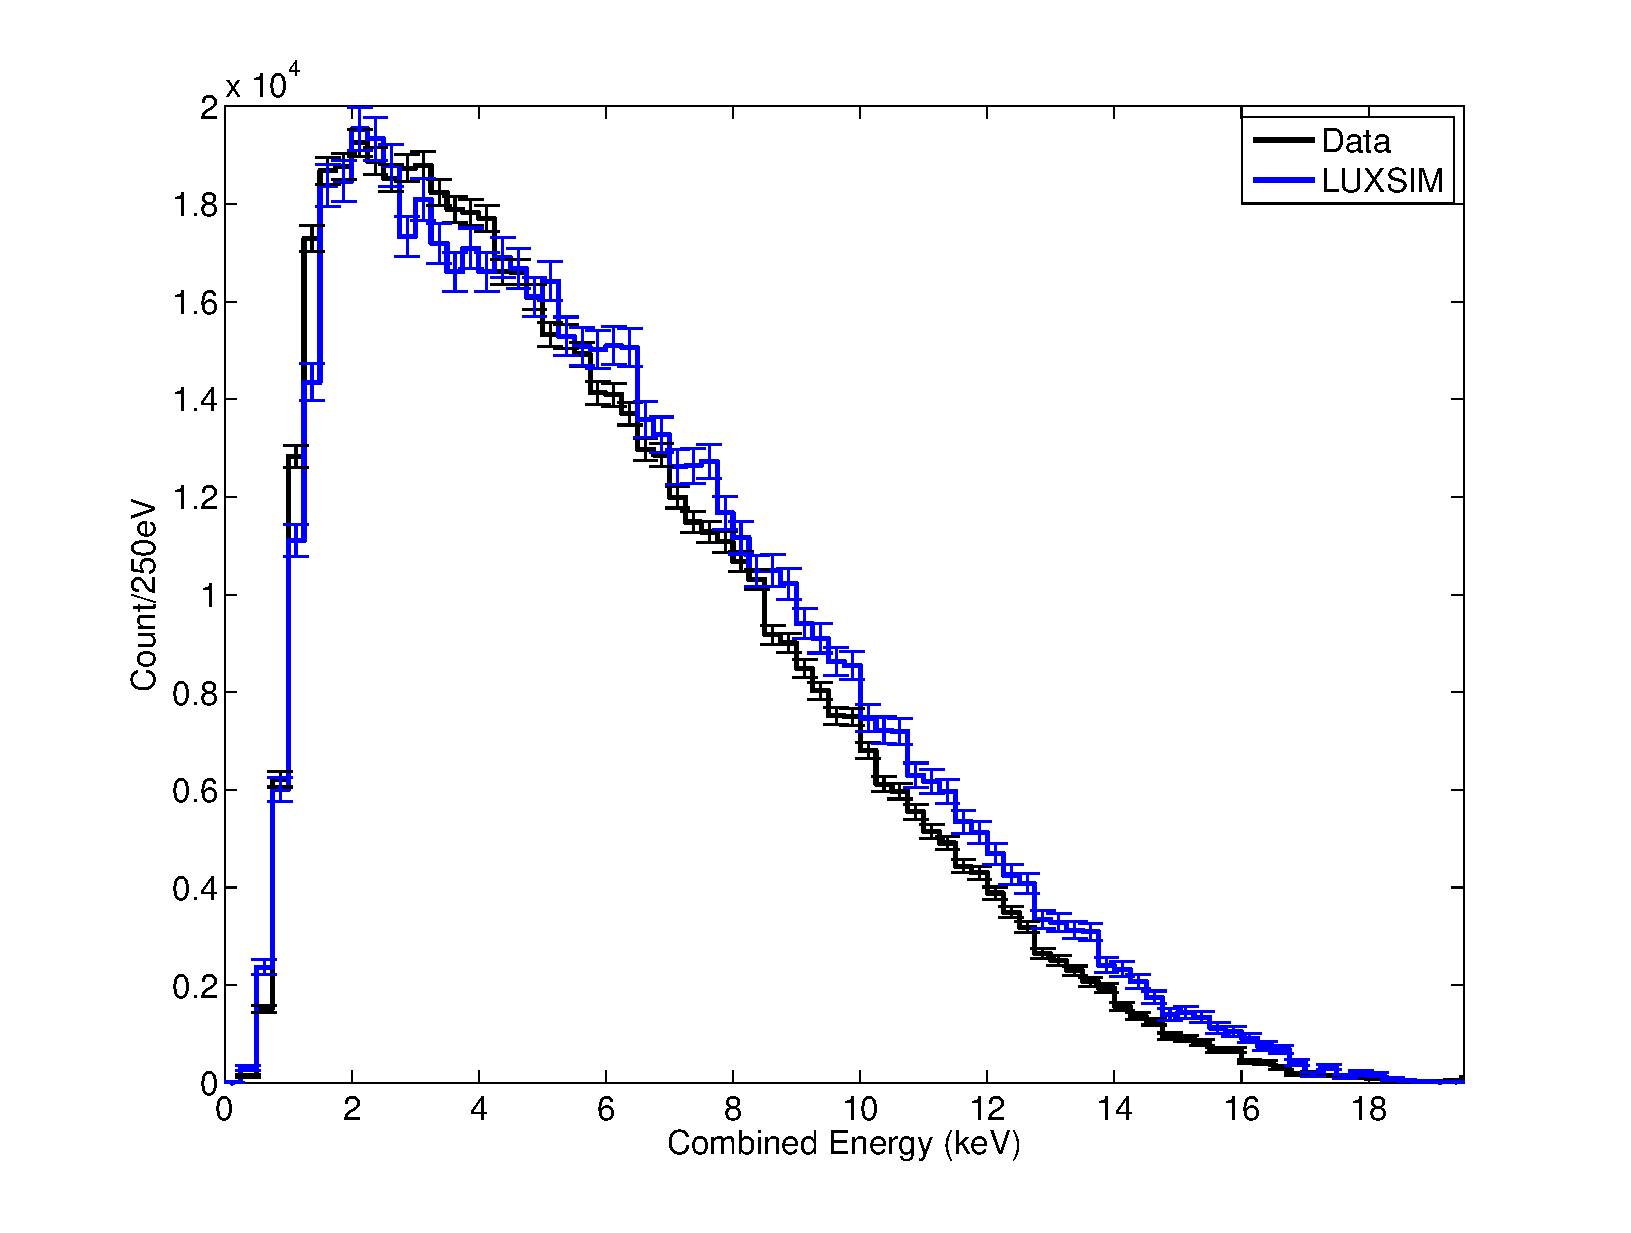
\includegraphics[width=80mm]{CH3T_E_spec_18_Tritium_Dec_2013_180.eps}
\caption{Combined energy spectrum of the tritium data and LUX SIM.}
\label{fig:E_spec}
\end{figure}
 


 
 \subsection{Absolute Rate}
The absolute efficiency for detecting tritium events can be determined by comparing the number of observed events to the number expected. The initial activity injected was calculated to be $0.84 \pm 0.22 $ Bq, with the largest uncertainty coming from the ratio of $\rm CH_3T/CH_4$ from the tritiated methane source bottle. The purification time constant was measured to be 6.6 hours. From the initial rate and the purification constant we expect to count a total of $20,200 \pm 4,000 $ events in the LUX detector before applying the S1 threshold. With the S1 threshold we expect  $16,000 \pm 3,100 $ `golden' events. The actual count observed in the liquid xenon volume was 20,000 events, which is in good agreement with the expected value taking into account the uncertainty in the initial activity and the purification model. After making fiducial cut $7,700 \pm  1,500$ events were expected and a total of $9,500 \pm 100$ were observed.
%,  roughly $16,000 \pm  3,100 * (290/324)*(18^2/24.5^2)$. 



\section{Scintillation Yield and Ionization Yield from Tritium Beta Decay}


\subsection{Cuts used in this analysis}
\begin{itemize}
\item Standard LUX Pulse finder classifier used in the WIMP search.
\item $\rm S2_b > 100 [Phe] $
\item PDE (g1) = 0.138 $\rm \pm 0.005$, measured with Tritium
\item Extraction = 0.664 $\rm \pm 0.04$ measured with Tritium.
\item single e- = 9.95 $\rm \pm 0.1$ [Phe/e-]
\item Using NEST 4c bands.
\end{itemize}




Scintillation and ionization yield are measured using the tritiated methane calibration source from the S1, S2 and reconstructed energy of each beta decay. The energy of each decay is determined using a prescription described in [Erik Dahl], see equations \ref{eq:Gain} and \ref{eq:E_comb}. 
\begin{equation}
\begin{split}
\rm  n_\gamma = \frac{S1}{g1}\\
\rm n_{e^{-}} = \frac{S2}{g2}
\label{eq:Gain}
\end{split}
\end{equation}

\begin{equation}
\begin{split}
\rm E= \frac{1}{W}(n_\gamma + n_{e^-})\\
\rm E= \frac{1}{W}(\frac{S1}{g1} + \frac{S2}{g2})
\label{eq:E_comb}
\end{split}
\end{equation}

The values of the work function W and gains g1, g2 have been measured using other calibration sources and are energy independent [ref]. Using equations \ref{eq:Gain} and \ref{eq:E_comb} we calculate the number of photons and electrons along with the energy of each tritium beta decay event to determine the yields. Scintillation and ionization yield are defined as [Photons/keV] and [Electrons/keV] respectively and the tritiated methane calibration source provides betas ranging from $\rm>1$ to 18 keV, with an exponential decline in event rate above 5 keV. For the results shown in figure \ref{fig:L_Q_Yield_180} over 150,000 beta decays in the fiducial volume were used to measure scintillation and ionization yield at 180 [V/cm]. A correction was applied for the beta spectral shape and the finite resolution of S1, S2 when measuring ionization and scintillation yield, the correction was found to be less than 10\% and is described in [my thesis]. Figure \ref{fig:L_Q_Yield_180} also shows the comparison of the results with the NEST model which has been vetted between 2 and 10 $\rm keV{ee}$. Also show are the measurements of light yield from a $\rm^{83m}Kr$ source, the 32.1 keV decay from $\rm^{83m}Kr$ is typically used as a standard calibration. (The second 9.4 keV decay from $\rm^{83m}Kr$  shown in the figure is for decays that occur more than 1000 ns after the initial 32.1 keV decay).

We find good agreement with the NEST model in the regions that have been vetted (2-10 $\rm keV{ee}$), see figure \ref{fig:L_Q_Yield_180}. Below 2 $\rm keV{ee}$ the light yield is lower than predicted by NEST and the charge yield is higher. The discrepancy between the data and the NEST model above 10 $\rm keV{ee}$ is due to limited data available for the model and also due to the track lengths of betas and gammas beginning to deviate above this energy. Note, under 10 $\rm keV{ee}$ track lengths of betas gammas are nearly identical. 

Figure \ref{fig:L_Q_Yield_Baudis} includes our light and charge yield measurements at 100 and 180 V/cm along with the recent Compton scattering measurement down to 1.5 $\rm keV{ee}$ from \cite{Baudis} at 450 V/cm. The error bars show in the figure include uncertainties from W, g1, g2 and the spectral shape correction. Unlike the measurement made using Compton scattering we can reconstruct energy using both the light and charge channels for each decay allowing for a powerful calibration down to 1 $\rm keV{ee}$ (corresponding to 80\% threshold at 2 Phe in S1).  We find a lower light yield than the centroids of the measurements in [ref Budias], however the the measurement is within reported errors. At our lower fields a higher light yield is expected than that measured at 450 V/cm due to less free charge separation.  The light yield of the 32.1 keV gamma from $\rm^{83m}Kr$ is shown on the figure as a measure of systematic uncertainty between the experiments. For the case of the standardized $\rm^{83m}Kr$ calibration source we find the expected behavior between the two experiments, a higher extraction field leads to lower light yield.

%\begin{figure}[h!]\centering
%\includegraphics[width=120mm]{LY_c_180_Tritium_Dec_2013_Charge_Yield_180_corr.png}
%\includegraphics[width=120mm]{CH3T_fid_E_S2_c_Tritium_Dec_2013_Charge_Yield_180_corr.png}
%\caption{Top: Scintillation yield vs. combined energy using tritium beta decay. Bottom: Ionization yield vs. combined energy using tritium beta decay. At a drift field of 180 [V/cm], in the fiducial volume, and containing over 150,000 beta decays. The endpoint of the tritium beta spectrum is 18.6 [keV]}
%\label{fig:L_Q_Yield}
%\end{figure}


 \begin{figure}[h!]\centering
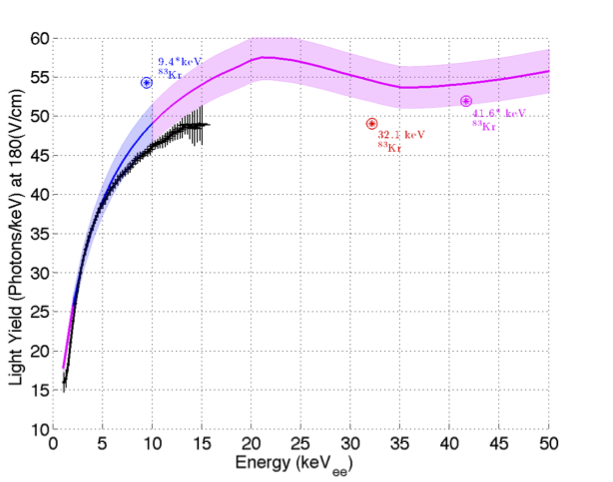
\includegraphics[width=80mm]{LY_180_band_Tritium_Dec_2013_Charge_Yield_180_corr.png}
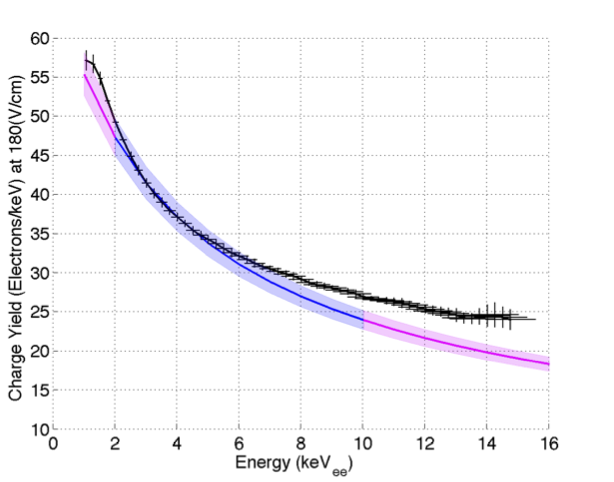
\includegraphics[width=80mm]{QY_180_Tritium_Dec_2013_Charge_Yield_180_corr.png}
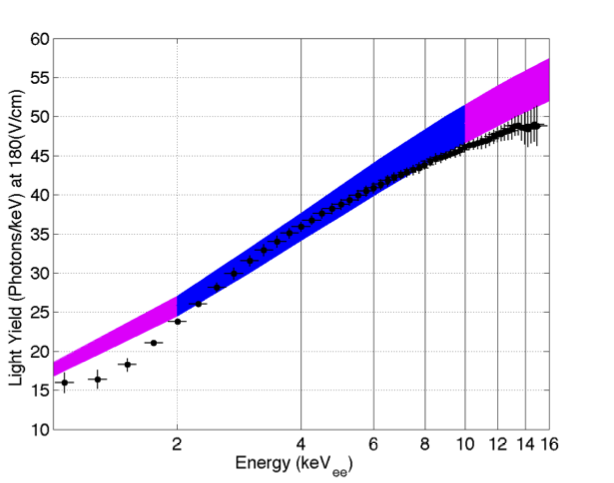
\includegraphics[width=80mm]{LY_180_band_log_Tritium_Dec_2013_Charge_Yield_180_corr.png}
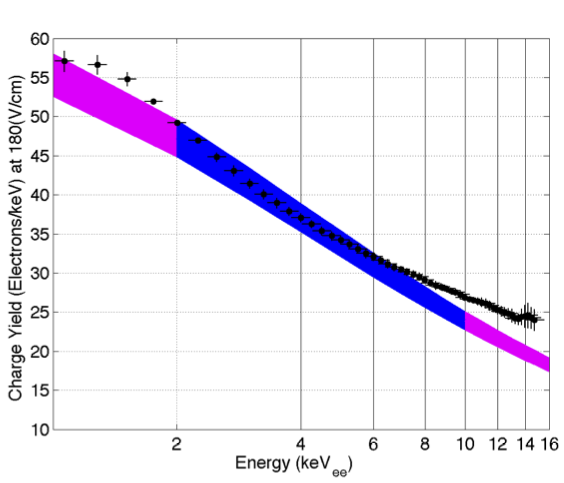
\includegraphics[width=76mm]{QY_180_log_Tritium_Dec_2013_Charge_Yield_180_corr.png}
\caption{180 [V/cm], corrected for spectral shape. Top Left: Mean scintillation yield vs. combined energy using tritium beta decay (black line). $\rm^{83}Kr$ lines are plotted for reference but only the 32.1 [keV] line (red star) is kosher since the 9.4 [keV] line is dependent on timing separation, the 9.4 [keV] line is plotted (blue star) for separations greater than 1000 [ns]. Top Right: Mean ionization yield vs. combined energy (black line). Bottom Left: Scintillation yield vs. combined energy on a log scale. Bottom Right: Ionization yield vs. combined energy on a log scale. The shaded blue regions represent the NEST mean with $\pm 5\%$ that has been vetted by data [Erik Dahl Thesis]. The shaded magenta regions represent the NEST extrapolations from data. The measurement is made at a field of 180 [V/cm] and contains over 150,000 beta decays. The endpoint of the tritium beta spectrum is 18.6 [keV]}
\label{fig:L_Q_Yield_180}
\end{figure}




 \begin{figure}[h!]\centering
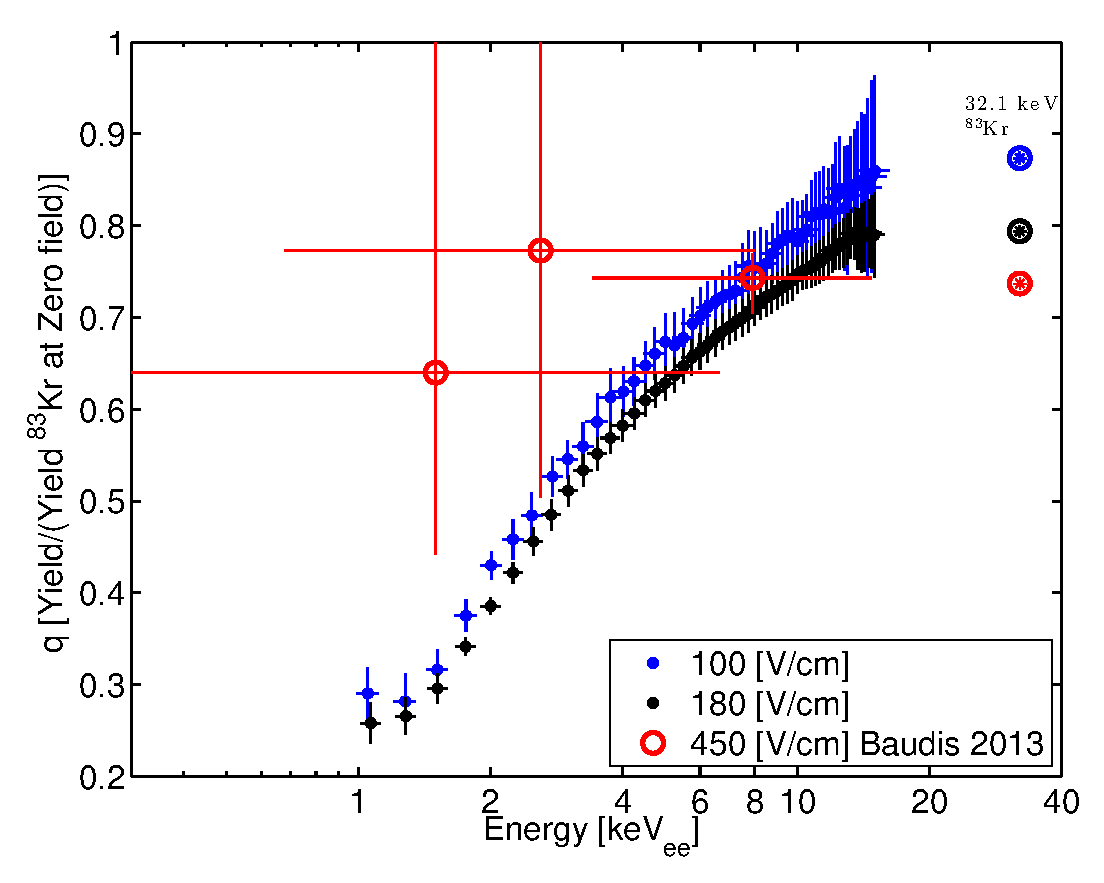
\includegraphics[width=80mm]{q_all_log_Tritium_Dec_2013_Charge_Yield_180_corr.eps}
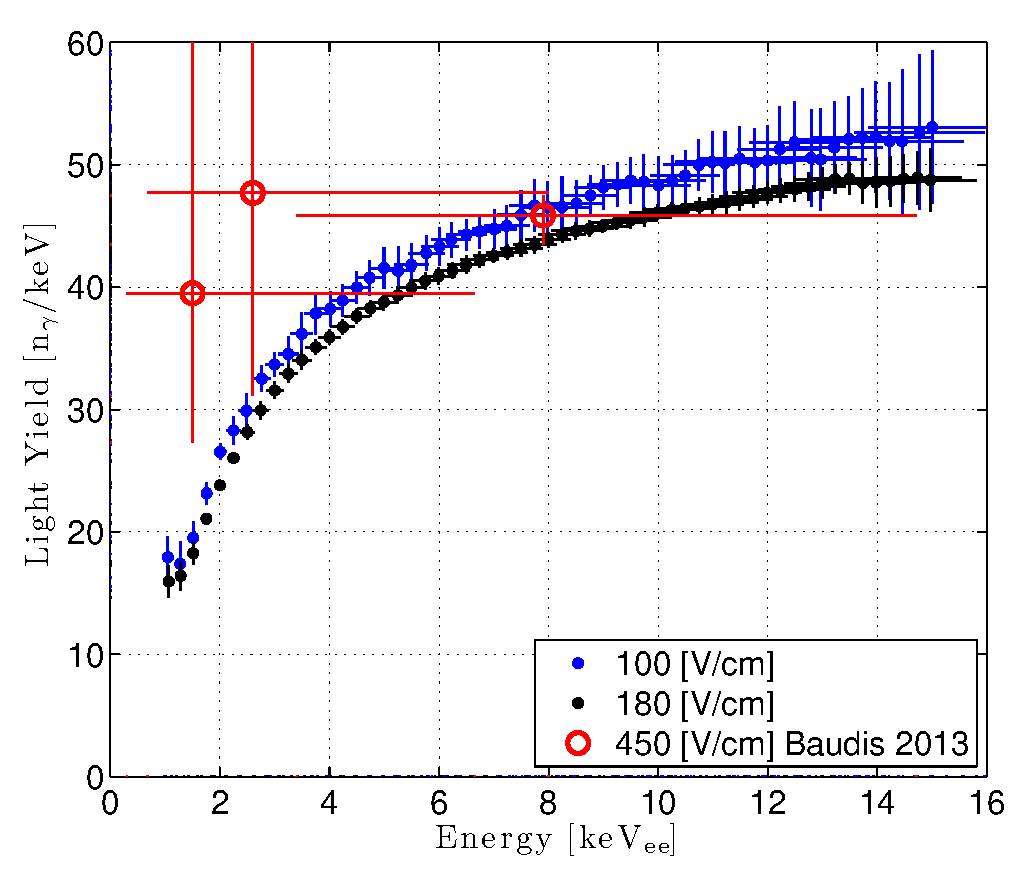
\includegraphics[width=80mm]{LY_all_Tritium_Dec_2013_Charge_Yield_180_corr.eps}
\includegraphics[width=80mm]{Charge_Y_all_Tritium_Dec_2013_Charge_Yield_180_corr.eps}
\caption{Top: Scintillation yield relative to the yield of the 32.1 gamma of [keV] $\rm^{83}Kr $  vs. Energy. Shaded blue curve is tritium at 100 [V/cm], shaded black curve is tritium at 180 [V/cm], red points represent a recent Compton scattering measurement at 450 [V/cm]. Also shown are the corresponding quenching of the 32.1 [keV]  gamma of $\rm^{83}Kr$ (star inside circle). Bottom: scintillation yield [Photons/keV] vs. Energy. Shaded blue curve is tritium at 100 [V/cm], shaded black curve is tritium at 180 [V/cm], red circles represent a recent Compton scattering measurement at 450 [V/cm].}
\label{fig:L_Q_Yield_Baudis}
\end{figure}



\end{comment}
%%%%%%%%%%%%%%%%%%%%%%%%%%%%%%%%%%%%%%%%%%%%%%%%%%%%%%%%%%

\section{All the things we can do with Tritium}

\begin{itemize}
\item Define the ER band.
\item Binned leakage fraction, and potentially optimize for spacial dependent leakage fraction in XYZ plane.
\item S1, S2 threshold. (Energy is a bit convoluted let's not go there). Requires NEST
\item Combined energy calibration to about 0.5 keVee. Requires NEST
\item Light Yield, Charge Yield. Requires some trivial smearing model, 10\% effect.
\item Fano-like factor vs. energy. Requires some trivial smearing model, sub 2\% effect.
\item Fiducial mass calculation, optimized for low energy S2s making it more WIMP like.
\item g1 and g2 calculation by competing tritium spectrum with NEST, or multiple E fields
\item ER band Gaussianity.
\item ... anything else?
\end{itemize}






\section{Summary}

We have characterized the electron recoil band and threshold of the LUX dark matter experiment with a tritium calibration source. The large dataset, high event purity, and simple topology provide a powerful tool to study the detector and to investigate the fundamental properties of LXe as a particle detection medium. The results presented here are used in an improved analysis of the Run 3 WIMP search data in Ref. \cite{lux-reanalysis}.

\begin{thebibliography}{1}

\bibitem{McKinsey} McKinsey, et al.  \emph{Journal of Physics: Conference Series} 203:012026 (2010) 
\bibitem{Fiorucci} Fiorucci, et al.  \emph{AIP Conference Proceedings} 1200:977 (2010)
\bibitem{Kastens} Kastens, et al. \emph{Phys. Rev. C} 80:045809 (2009)
\bibitem{Miyake} Miyake, et al.  \emph{J. vac. Sci. technol. A.} 1:1446-1451 (1983)
\bibitem{Piche} R. Piche. \emph{Partial Differential Equations} Tampere University of Technology.
\bibitem{Flanconneche} B. Flanconneche, J. Martin and M.H. Klopffer. "Permeability, Diffusion and Solubility of Gases in Polyethylene, Polyamide 11 and Poly(vinylidene fluoride)." \emph{Oil and Gas Technology}. Vol 1. 2001. p 261-278.


\end{thebibliography}


\end{document}



%\bibliography{Tritium}

\end{document}